% !TeX root = Thesis.tex
\documentclass[11pt]{mimosis}
\synctex=1

% \PassOptionsToClass{14pt}{scrbook}
\usepackage{metalogo}

\usepackage{textcomp}
\usepackage{gensymb}

\usepackage[pass]{geometry}

%%%%%%%%%%%%%%%%%%%%%%%%%%%%%%%%%%%%%%%%%%%%%%%%%%%%%%%%%%%%%%%%%%%%%%%%
% Some of my favorite personal adjustments
%%%%%%%%%%%%%%%%%%%%%%%%%%%%%%%%%%%%%%%%%%%%%%%%%%%%%%%%%%%%%%%%%%%%%%%%
%
% These are the adjustments that I consider necessary for typesetting
% a nice thesis. However, they are *not* included in the template, as
% I do not want to force you to use them.

% This ensures that I am able to typeset bold font in table while still aligning the numbers
% correctly.
\usepackage{etoolbox}

\usepackage[binary-units=true]{siunitx}
\DeclareSIUnit\px{px}

\sisetup{%
  detect-all           = true,
  detect-family        = true,
  detect-mode          = true,
  detect-shape         = true,
  detect-weight        = true,
  detect-inline-weight = math,
}

%%%%%%%%%%%%%%%%%%%%%%%%%%%%%%%%%%%%%%%%%%%%%%%%%%%%%%%%%%%%%%%%%%%%%%%%
% Hyperlinks & bookmarks
%%%%%%%%%%%%%%%%%%%%%%%%%%%%%%%%%%%%%%%%%%%%%%%%%%%%%%%%%%%%%%%%%%%%%%%%

\usepackage[%
  colorlinks = true,
  citecolor  = BrickRed,
  linkcolor  = BrickRed,
  urlcolor   = BrickRed,
  % pdftex,
  pdfauthor={Guybrush Threepwood},
  pdftitle={Reflections on the correlation between the tendency to procrastinate and the likelihood to be awarded a doctoral degree},
  % pdfsubject={The Subject},
  % pdfkeywords={Some Keywords},
  % pdfproducer={Latex with hyperref, or other system},
  % pdfcreator={pdflatex, or other tool}
  final,
  ]{hyperref}

\usepackage{bookmark}


%%%%%%%%%%%%%%%%%%%%%%%%%%%%%%%%%%%%%%%%%%%%%%%%%%%%%%%%%%%%%%%%%%%%%%%%
% Bibliography
%%%%%%%%%%%%%%%%%%%%%%%%%%%%%%%%%%%%%%%%%%%%%%%%%%%%%%%%%%%%%%%%%%%%%%%%
%
% I like the bibliography to be extremely plain, showing only a numeric
% identifier and citing everything in simple brackets. The first names,
% if present, will be initialized. DOIs and URLs will be preserved.

\usepackage[%
  autocite      = plain,
  backend       = biber,
  doi           = false,
  url           = true,
  giveninits    = true,
  hyperref      = true,
  maxbibnames   = 99,
  maxcitenames  = 99,
  sortcites     = true,
  style         = alphabetic,
  citestyle     = alphabetic,
  maxalphanames = 4,           % max number of authors before it becomes [First+12]
  backref       = true,
  ]{biblatex}


%%%%%%%%%%%%%%%%%%%%%%%%%%%%%%%%%%%%%%%%%%%%%%%%%%%%%%%%%%%%%%%%%%%%%%%%
% Some adjustments to make the bibliography more clean
%%%%%%%%%%%%%%%%%%%%%%%%%%%%%%%%%%%%%%%%%%%%%%%%%%%%%%%%%%%%%%%%%%%%%%%%
%
% The subsequent commands do the following:
%  - Removing the month field from the bibliography
%  - Fixing the Oxford commma
%  - Suppress the "in" for journal articles
%  - Remove the parentheses of the year in an article
%  - Delimit volume and issue of an article by a colon ":" instead of
%    a dot ""
%  - Use commas to separate the location of publishers from their name
%  - Remove the abbreviation for technical reports
%  - Display the label of bibliographic entries without brackets in the
%    bibliography
%  - Ensure that DOIs are followed by a non-breakable space
%  - Use hair spaces between initials of authors
%  - Make the font size of citations smaller
%  - Fixing ordinal numbers (1st, 2nd, 3rd, and so) on by using
%    superscripts

% Remove the month field from the bibliography. It does not serve a good
% purpose, I guess. And often, it cannot be used because the journals
% have some crazy issue policies.
\AtEveryBibitem{\clearfield{month}}
\AtEveryCitekey{\clearfield{month}}

% Fixing the Oxford comma. Not sure whether this is the proper solution.
% More information is available under [1] and [2].
%
% [1] http://tex.stackexchange.com/questions/97712/biblatex-apa-style-is-missing-a-comma-in-the-references-why
% [2] http://tex.stackexchange.com/questions/44048/use-et-al-in-biblatex-custom-style
%
\AtBeginBibliography{%
  \renewcommand*{\finalnamedelim}{%
    \ifthenelse{\value{listcount} > 2}{%
      \addcomma
      \addspace
      \bibstring{and}%
    }{%
      \addspace
      \bibstring{and}%
    }
  }
}

% Suppress "in" for journal articles. This is unnecessary in my opinion
% because the journal title is typeset in italics anyway.
\renewbibmacro{in:}{%
  \ifentrytype{article}
  {%
  }%
  % else
  {%
    \printtext{\bibstring{in}\intitlepunct}%
  }%
}

% Remove the parentheses for the year in an article. This removes a lot
% of undesired parentheses in the bibliography, thereby improving the
% readability. Moreover, it makes the look of the bibliography more
% consistent.
\renewbibmacro*{issue+date}{%
  \setunit{\addcomma\space}
    \iffieldundef{issue}
      {\usebibmacro{date}}
      {\printfield{issue}%
       \setunit*{\addspace}%
       \usebibmacro{date}}%
  \newunit}

% Delimit the volume and the number of an article by a colon instead of
% by a dot, which I consider to be more readable.
\renewbibmacro*{volume+number+eid}{%
  \printfield{volume}%
  \setunit*{\addcolon}%
  \printfield{number}%
  \setunit{\addcomma\space}%
  \printfield{eid}%
}

% Do not use a colon for the publisher location. Instead, connect
% publisher, location, and date via commas.
\renewbibmacro*{publisher+location+date}{%
  \printlist{publisher}%
  \setunit*{\addcomma\space}%
  \printlist{location}%
  \setunit*{\addcomma\space}%
  \usebibmacro{date}%
  \newunit%
}

% Ditto for other entry types.
\renewbibmacro*{organization+location+date}{%
  \printlist{location}%
  \setunit*{\addcomma\space}%
  \printlist{organization}%
  \setunit*{\addcomma\space}%
  \usebibmacro{date}%
  \newunit%
}

% Do not abbreviate "technical report".
\DefineBibliographyStrings{english}{%
  techreport = {technical report},
}

% Display the label of a bibliographic entry in bare style, without any
% brackets. I like this more than the default.
%
% Note that this is *really* the proper and official way of doing this.
\DeclareFieldFormat{labelnumberwidth}{#1\adddot}

% Ensure that DOIs are followed by a non-breakable space.
\DeclareFieldFormat{doi}{%
  \mkbibacro{DOI}\addcolon\addnbspace
    \ifhyperref
      {\href{http://dx.doi.org/#1}{\nolinkurl{#1}}}
      %
      {\nolinkurl{#1}}
}

% Use proper hair spaces between initials as suggested by Bringhurst and
% others.
\renewcommand*\bibinitdelim {\addnbthinspace}
\renewcommand*\bibnamedelima{\addnbthinspace}
\renewcommand*\bibnamedelimb{\addnbthinspace}
\renewcommand*\bibnamedelimi{\addnbthinspace}

% Make the font size of citations smaller. Depending on your selected
% font, you might not need this.
\renewcommand*{\citesetup}{%
  \biburlsetup
  \small
}

% \DeclareLanguageMapping{british}{bibliography-correct-ordinals}
% \DeclareLanguageMapping{english}{bibliography-correct-ordinals}
\bibliography{Thesis}

%%%%%%%%%%%%%%%%%%%%%%%%%%%%%%%%%%%%%%%%%%%%%%%%%%%%%%%%%%%%%%%%%%%%%%%%
% Fonts
%%%%%%%%%%%%%%%%%%%%%%%%%%%%%%%%%%%%%%%%%%%%%%%%%%%%%%%%%%%%%%%%%%%%%%%%

\ifxetexorluatex
  %\setmainfont{Minion Pro}
  \usepackage{microtype}
\else
  %\usepackage[osf,lining]{ebgaramond}  
  \usepackage[scale=0.7]{sourcecodepro}  
\fi


\usepackage{amsmath}
\usepackage{mathpazo}
\usepackage{lettrine}
\usepackage{tikz}
\usepackage{wrapfig}
\usepackage{pgfplots}
\usepackage[justification=centering]{caption}
\usepackage{framed}
\pgfplotsset{compat=newest}

% \usepackage{minipage}

\usepackage{makeidx}
\makeindex



% \newacronym[description={Principal component analysis}]{PCA}{PCA}{principal component analysis}
% \newacronym                                            {SNF}{SNF}{Smith normal form}
% \newacronym[description={Topological data analysis}]   {TDA}{TDA}{topological data analysis}

% \makeindex
% \makeglossaries

%%%%%%%%%%%%%%%%%%%%%%%%%%%%%%%%%%%%%%%%%%%%%%%%%%%%%%%%%%%%%%%%%%%%%%%%
% Incipit
%%%%%%%%%%%%%%%%%%%%%%%%%%%%%%%%%%%%%%%%%%%%%%%%%%%%%%%%%%%%%%%%%%%%%%%%
 
\usepackage{mathtools}
\usepackage{amssymb}
\usepackage{siunitx}

\usepackage{blindtext}

% Corrects \autoref{}: chapter -> Chapter, section -> Section, subsection -> Section
\addto\extrasenglish{%
  \renewcommand{\chapterautorefname}{Chapter}%
  \renewcommand{\sectionautorefname}{Section}%
  \renewcommand{\subsectionautorefname}{Section}%
}

\begin{document}

\frontmatter
  %!TEX root = ../Thesis.tex

\begin{titlepage}
  \centering % Center all text
  \vspace*{\baselineskip} % White space at the top of the page

  %\rule{\textwidth}{1.6pt}\vspace*{-\baselineskip}\vspace*{2pt} % Thick horizontal line
  %\rule{\textwidth}{0.4pt}\\[1.0\baselineskip] % Thin horizontal line

  {\huge Time-Coherent Streamline Placement}\\[0.2\baselineskip] % Title

  %\rule{\textwidth}{0.4pt}\vspace*{-\baselineskip}\vspace{3.2pt} % Thin horizontal line
  %\rule{\textwidth}{1.6pt}\\ % Thick horizontal line

  \vspace*{\baselineskip}

  {\Large Bachelor's Thesis\\[\baselineskip]} % Tagline(s) or further description
  \vspace*{\baselineskip}

  {\LARGE Alexander Baucke\\[\baselineskip]} % Editor list  

  \vspace*{\baselineskip} % Whitespace between location/year and editors

  Supervisor\\
  {\large  Prof.\,Dr.\,Filip Sadlo\\[\baselineskip]} % Editor list

  \vfil

  Heidelberg, Germany,  \today \par % Location and year

  \vspace*{\baselineskip}

  {\itshape Faculty of Mathematics and Computer Science\par} % Editor affiliation
  {\itshape Heidelberg University\par} % Editor affiliation
\end{titlepage}

\cleardoublepage

  % %!TEX root = ../Thesis.tex

\selectlanguage{english}

\begin{titlepage}
  \begin{center}
    \textsc{\huge Dissertation}
                \vskip 1cm
                \begin{large}
                  submitted to the\\[0.50cm]
                  \begin{Large}
                    \textsc{Combined Faculty for the\\Natural Sciences and Mathematics}\\[0.50cm]
                  \end{Large}
                  of\\[0.50cm]
                  \begin{Large}
                    \textsc{Heidelberg University, Germany}\\[0.50cm]
                  \end{Large}
                  for the degree of \\[0.5cm] 
                  Doctor of Natural Sciences
                \end{large}
    %
    \vfill
    %
    \begin{large}
                  put forward by\\[0.5cm]
                  \begin{LARGE}
                    \textbf{Guybrush Threepwood}, M.Sc.
                  \end{LARGE}\\[0.5cm]
                  born in Ankh-Morpork, Discworld
    \end{large}
    %
    \vskip 2cm
    %
    \begin{small}
      Heidelberg\\
      Marchtember 2033
    \end{small}
  \end{center}
\end{titlepage}

\selectlanguage{english}

\begin{titlepage}
  %
  \phantom{}
  \vfill 
  %
  \begin{center}
    \begin{singlespace*}
      \begin{Huge}
          Reflections on the correlation between the tendency to procrastinate and the likelihood to be awarded a doctoral degree\par
      \end{Huge}
      %
      \vskip 0.25cm
      \emph{by}
      \vskip 0.25cm
      %
      \textsc{Guybrush Threepwood}\par
    \end{singlespace*}
  \end{center}
  %
  \vfill
  %
  \begin{singlespace*}
    Advisor:            Prof.\,Dr.\,Filip Sadlo \\[.5cm]
    Oral examination: \rule{4cm}{0.15mm}
  \end{singlespace*}
\end{titlepage}

\newpage
\null
\thispagestyle{empty}
\newpage
  % for PhD thesis
  \pagestyle{empty}
  %!TEX root = ../Thesis.tex

\section*{Declaration of Authorship}

% Official declaration of authorship from the Institute for Computer Science in german from https://www.informatik.uni-heidelberg.de/studium/thesis-erklaerung?lang=de
%Hiermit versichere ich, dass ich die Arbeit selbst verfasst und keine anderen als die angegebenen Quellen und Hilfsmittel benutzt und wörtlich oder inhaltlich aus fremden Werken Übernommenes als fremd kenntlich gemacht habe. Ferner versichere ich, dass die übermittelte elektronische Version in Inhalt und Wortlaut mit der gedruckten Version meiner Arbeit vollständig übereinstimmt. Ich bin einverstanden, dass diese elektronische Fassung universitätsintern anhand einer Plagiatssoftware auf Plagiate überprüft wird.

% Official declaration of authorship from the Institute for Computer Science from https://www.informatik.uni-heidelberg.de/studium/thesis-erklaerung?lang=en
I hereby certify that I have written the work myself and that I have not used any sources or aids other than those specified and that I have marked what has been taken over from other people's works, either verbatim or in terms of content, as foreign. I also certify that the electronic version of my thesis transmitted completely corresponds in content and wording to the printed version. I agree that this electronic version is being checked for plagiarism at the university using plagiarism software.

% Old version
%I hereby declare that the thesis submitted is my own unaided work. All direct or indirect sources used are acknowledged as references. The principles and recommendations \enquote{Verantwortung in der Wissenschaft} of Heidelberg University have been followed.
\vspace{5cm}
\noindent\rule[0.5ex]{8em}{0.5pt} \hfill \rule[0.5ex]{10em}{0.5pt}\\
\noindent first and last name \hfill city, date and signature  % remove for PhD thesis
  %!TEX root = ../Thesis.tex

\begin{center}
  \textsc{Abstract}
\end{center}
% Grammarly'd
\noindent
Common elements in visualizing steady vector fields are integral lines that show flow dynamics, called streamlines.
Many possible criteria can define the quality of a set of streamlines when visualizing a vector field.
Frequently used placement properties include the uniformity and length of the streamlines, with even spacing and maximum length being the preferred choice for high visual appeal.
We have noticed that the most relevant criterion for visualizing $unsteady$ fields using e.g.,
animations, is largely unaccounted for.
Currently, most algorithms can only animate a vector field frame-by-frame without time-awareness.
The result is many visually pleasing images lacking coherence between each other,
as said algorithms place streamlines merely to fulfill the frame-limited optimum.
We overcome this problem by introducing an algorithm capable of time-coherent streamline placement,
effectively minimizing streamline movement between frames.
We implement an image-guided approach based on the work by Greg Turk and David Banks \cite{TurkBanks} to
generate initial streamline placements according to the above criteria.
To add time coherence, several key changes to different components are made.
The first change revolves around the energy measure, a function defining
the uniformity of streamline placement by comparing it with a target brightness.
Another change is the kernel Turk and Banks use to blur the image,
which we adapt to include time coherence, as well as introducing a new seeding strategy.
We show how the individual changes affect the streamline placement locally and globally,
and apply the algorithm to various datasets.
\cleardoublepage

  %!TEX root = ../Thesis.tex

\begin{center}
  \textsc{Zusammenfassung}
\end{center}
%
\selectlanguage{ngerman}
Ziel dieser Arbeit ist das Erreichen von Zeitkohärenz bei Stromlinien
in zeitabhängigen Vektorfeldern, um deren Darstellung durch z.B. Animationen zu verbessern.
Wir beginnen mit einer Definition für Zeitkohärenz, die im Wesentlichen auf die
Bewegung einer Stromlinie von einem Zeitschritt zum nächsten gestützt ist.
Wenn diese Bewegung groß ausfällt bzw. sich die Stromlinie viel bewegt hat,
bezeichnen wir dies als ``schlechte Zeitkohärenz''.
Wir zeigen, warum zeitkohärentes Verhalten wichtig ist für z.B. Animationen,
und entwickeln eine prototypische Implementierung, deren Parametrisierung
wir dann anhand einiger Beispiele bestimmen.
Unser Algorithmus basiert auf einer durch Bild-geleiteten Implementierung von Greg Turk und David Banks,
den wir durch einige Änderungen an den zentralen Komponenten zeitkohärent gemacht haben.
Im Anschluss werden einige Datensätze damit ausgewertet und mit anderen einfachen Algorithmen verglichen;
außerdem beschreiben wir einige Limitierungen sowie Ideen für Verbesserungen.
Zum Schluss wird eine kurze Komplexitätsanalyse durchgeführt und die Performance untersucht.
\selectlanguage{english}
\cleardoublepage

  \tableofcontents

\mainmatter
  \pagestyle{scrheadings}

  %!TEX root = ../Thesis.tex

%%%%%%%%%%%%%%%%%%%%%%%%%%%%%%%%%%%%%%%%%%%%%%%%%%%%%%%%%%%%%%%%%%%%%%%%
\chapter{Introduction}
%%%%%%%%%%%%%%%%%%%%%%%%%%%%%%%%%%%%%%%%%%%%%%%%%%%%%%%%%%%%%%%%%%%%%%%%

The visualization of vector fields is a heavily used component in many fields like aerospace engineering, geology, fluid dynamics, material science, or the biomedical sector.
Common examples include weather systems, rotor design, analysis of marker movement inside of cells, or the magnetic field of a star.
Displaying such fields in a human-focused way is invaluable when analyzing the underlying systems' dynamics, and allows for faster and more accurate data analysis.

Contemporary research is mostly focused on continuous and steady vector fields.
Lines are usually optimized with respect to a single frame, which in turn has a very pleasing appearance.
If we introduce small changes over time, i.e. use an unsteady vector field, it is unlikely those algorithms will prefer lines similar to the ones in the last frame.
This causes the streamlines to move about and shift between frames a lot more than the time-induced changes to the field would warrant.
The sporadic movement makes it very difficult to perceive the flow change of the field.
Therefore, creating an animation of an unsteady vector field's behavior is very difficult,
time-consuming, and requires a lot of human intervention in order to achieve good results.
This is extremely limiting, as most (if not all) vector fields represent a dynamic system.
Therefore, the focus of this thesis will be threefold:
\begin{itemize}
    \item How a lack of coherence of streamlines in different time steps of a continuous, unsteady field affects the visual quality of a field.
    A criterion to measure time coherence will also be presented.
    \item The implementation and underlying ideas of an image-based algorithm generating evenly-spaced long streamlines.
    \item Adaptations of the algorithm to allow a controlled bias between similarity to a previous time step, and optimality w.r.t. the current step.
\end{itemize}
We have chosen an image-based approach (opposed to a feature-guided one, see Section 2 for a disambiguation) for our work,
because the movement of lines in-between time frames is better suited for an appearance-focused algorithm.
Another reason is that feature-guided algorithms usually act locally, whereas the movement of a line from one step to another
is a global constraint.
The succeeding sections are structured as follows:
\begin{description}
    \item [Chapter 2] presents some recent developments and concepts.
    \item [Chapter 3] contains fundamentals about vector fields and streamlines.
    \item [Chapter 4] is about the base algorithm, the definition of a criterion for time coherence, and changes made to account for time coherence.
    \item [Chapter 5] contains the implementation and some design ideas.
    \item [Chapter 6] examines the individual changes' effects on different datasets, and we discuss issues, performance, and other measurements.
    \item [Chapter 7] concludes the thesis with some ideas for future work and improvements.
\end{description}

  %%%%%%%%%%%%%%%%%%%%%%%%%%%%%%%%%%%%%%%%%%%%%%%%%%%%%%%%%%%%%%%%%%%%%%%%
\chapter{Related Work}
\label{sec:relatedWork}
%%%%%%%%%%%%%%%%%%%%%%%%%%%%%%%%%%%%%%%%%%%%%%%%%%%%%%%%%%%%%%%%%%%%%%%%

Most of the works published in the field of streamline placement algorithms can be divided into two categories:
\subsection{Image-Guided}
The goal of this approach is to achieve a very uniform spacing of lines, giving an almost "hand-drawn" appearance.
Generated images will usually have high visual quality, at the risk of potentially missing or misrepresenting important features.
\\\\
One of the first and most prominent examples in this category was written by Greg Turk and David Banks~\cite{TurkBanks},
which we have adopted as the base for our algorithm as well.
In their research paper, a function (called the "Energy Function") is defined such that it maps an input image containing the potential streamlines to a scalar.
The scalar represents the quality of the image, roughly defined as the uniformity of the gray scales it contains. 
Adding/moving/removing/resizing streamlines is done randomly, at every step the energy function is used to determine whether a change gets accepted or discarded.
The algorithm is finished when the energy function reaches a lower energy bound, or a maximum number of consecutive rejected steps is exceeded.


\subsection{Feature-Guided}
Feature-Guided algorithms examine the underlying field structure before placing seeds.
They search for critical points or patterns in the field and then seed around them, capturing them in much higher detail.
The resulting images inherently represent the critical points much better, at the cost of some visual appeal compared to the aforementioned group.
\bigskip

\subsection{Other Relevant Works}
\begin{itemize}
    \item \href{https://www.cs.purdue.edu/homes/xmt/papers/Coherent-Streamline_Tsinghua_2012.pdf}{Time Coherence in 2D}
    \item \href{https://www.cg.tuwien.ac.at/courses/Visualisierung1/2015W/exercises/Streamlines_Jobard&Lefer.pdf}{Approach I've used so far due to simplicity}
\end{itemize}

Do not forget to use references~\cite{Hanser2019energy} like done here~\cite{Hofmann2019dependentVectors} to enable the bibliography~\cite{Jung2017tumble, Sagrista2019GaiaSky, Sdeo2018fullerene, Zheng2019equivalence}.
  %%%%%%%%%%%%%%%%%%%%%%%%%%%%%%%%%%%%%%%%%%%%%%%%%%%%%%%%%%%%%%%%%%%%%%%%
\chapter{Fundamentals}
\begin{figure}[ht]
    \centering
    \begin{subfigure}{.5\textwidth}
        \centering
        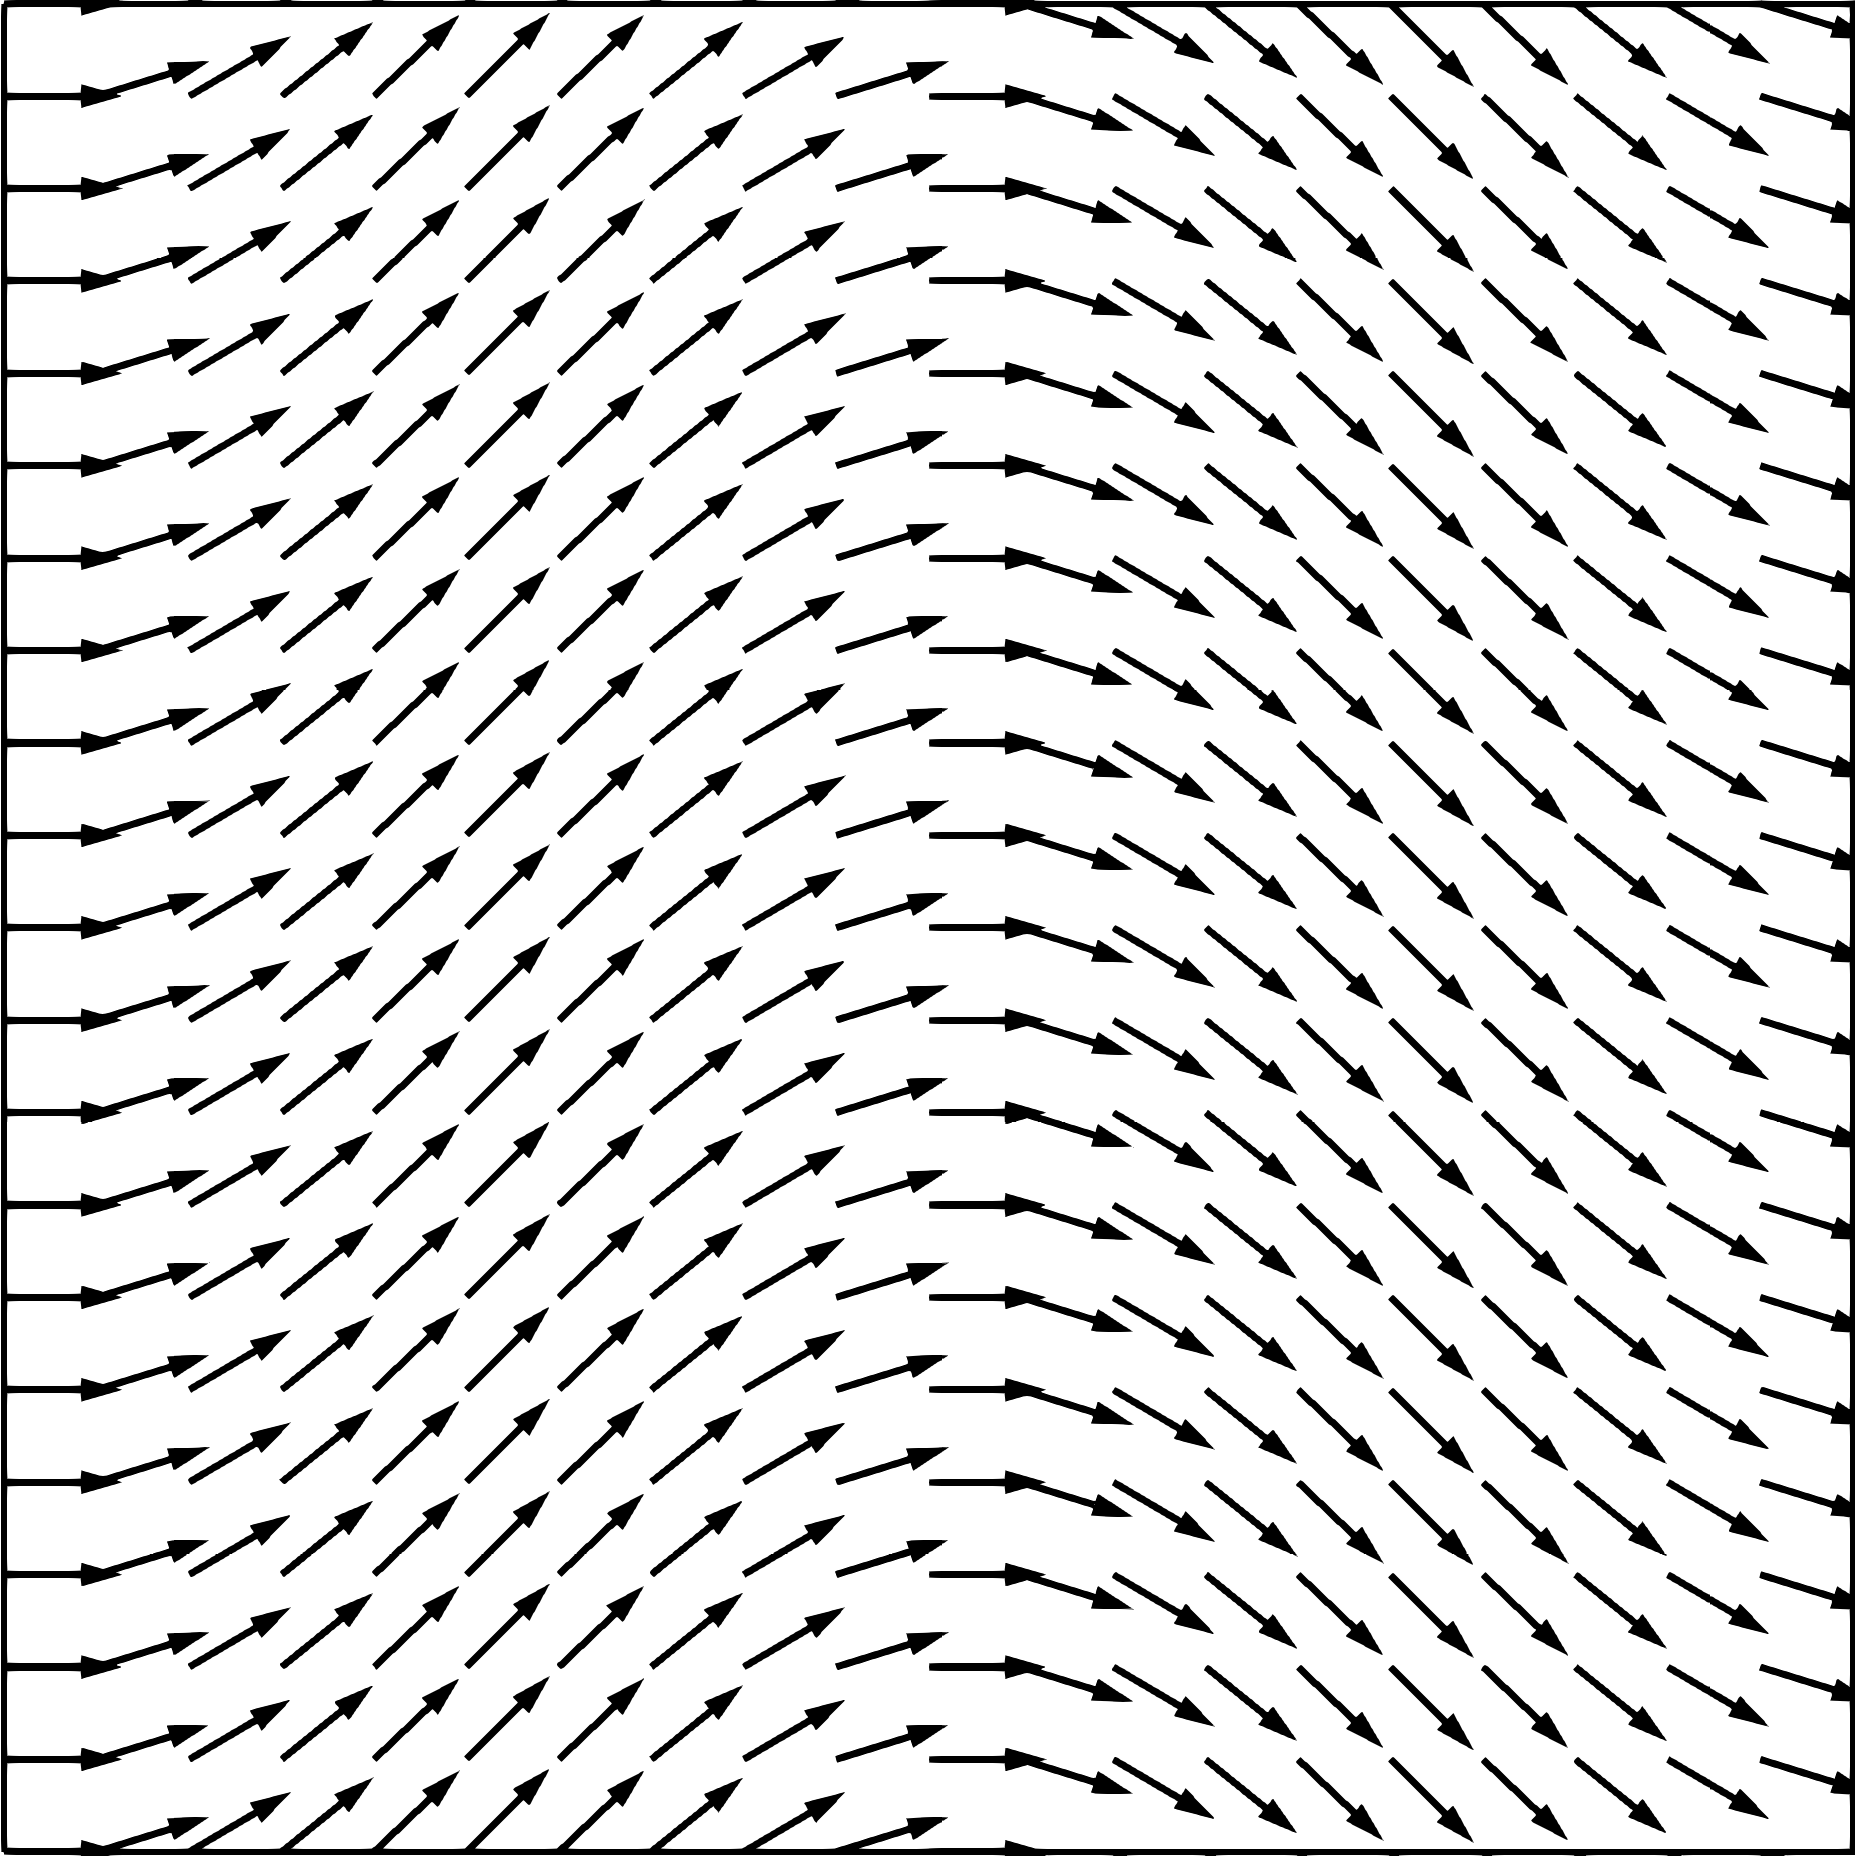
\includegraphics[scale=.1]{figures/WavesArrowField.png}
        \caption{A vector field defined by $u(x,y) = (1, \sin(x))^T$, visualized using arrows placed on a regular grid.}
    \end{subfigure}
    \label[figure]{fig:fundamentals_1}
\end{figure}
\noindent In this section, we describe the elementary components used in the remainder of this thesis.
Since this work is about the placement of streamlines in vector fields,
we start with the fundamentals of the field \textit{vector field visualization} in \Cref{sec:VFV}.
Our algorithm uses an image-guided base, hence we will also include some topics from the area of \textit{image processing} in \Cref{sec:IP}.
We conclude this chapter with a brief overview of the roots of unity in \Cref{sec:ROU},
because they are used in the development of an initial prototype in \Cref{sec:3D}.
%%%%%%%%%%%%%%%%%%%%%%%%%%%%%%%%%%%%%%%%%%%%%%%%%%%%%%%%%%%%%%%%%%%%%%%%
\section{Vector Field Visualization}
\label[section]{sec:VFV}
\paragraph*{Vector Field} A vector field represents how vectorized elements act over a spatial domain.
Concerning vector fields representing flow, this means that for every point in a domain, we can obtain the force acting at that point.

More formally, we can define a vector field as a map from $n$-dimensional scalars to $m$-dimensional scalars.
We can write it as an $n$-$m$-valued function, and in this thesis, we will only care about cases of $n=m$ in two and three dimensions.
There are several ways to obtain such fields, one is via an algebraic definition such as $u(x,y) = (1, \sin(x))^T$, giving us a field like the one seen in \Cref{fig:fundamentals_1}.
If we want our force to not only depend on spatial input but also on another scalar like a time component, we write this as $u(x,y,t)$ for the 2D case.       
We call vector fields \textit{steady} if they are not time-dependent; otherwise, we refer to them as \textit{unsteady}.
Another distinction is \textit{continuity}, which is analogous to the algebraic definition of other functions.
The fields in this work are all going to be continuous.

\paragraph*{Critical Points} A vector field can have points with distinct characteristics, called critical points.
In the 2D case, only four commonly used critical points exist, which we briefly describe here.
\begin{description}
    \item[Source]
    Given a field such as $u(x,y) = (x,y)$, at every point applies a force away from the origin.
    If we think about this as a non-compressible flow, this is equivalent to matter being created at the point $(0,0)$ and flowing outward.
    We refer to such a point as a \textit{source}.
    \item[Sink]
    Similarly, $u(x,y) = (-x,-y)$ would give us a \textit{sink} at $(0,0)$, equivalent to destroying liquid flowing inward.
    \item[Saddle]
    A saddle is an area where matter is pinched in one direction and stretched in another, e.g. in a field defined by $u(x,y) = (-x,y)$.
    \item[Periodic Orbit]
    $u(x,y) = (-y,x)$ creates circular paths around the origin where, after traveling a certain distance, a particle arrives at the point it started at.
    These critical points are called \textit{periodic orbits}.
\end{description}
\paragraph*{Streamlines}
Given a vector field $u$ and a point $P$, we can trace the movement of this point through $u$ by integrating over the field.
Intuitively, we can step through the field by choosing the next point $P_n = P_{n-1} + c \cdot u(P_{n-1})$, with $c$ being a step size scale.
If we do this an infinite number of times with $\pm c$ close to zero,
we end up with a set of points $S$ we have passed through, which defines the streamline.
$S$ has two notable properties:
\begin{itemize}
    \item Every point $P\in S$ inside this set has a velocity equal to $u(P)$.
    Hence, a streamline is tangent to the vector field at every point.
    \item No matter which point inside $S$ we use as $P_0$, we will always obtain the same set $S$ as its streamline.
    Therefore, any point inside $S$ is a potential \textit{seed} yielding the streamline $S$.
\end{itemize}
\newpage
\begin{figure}[t]
    \centering
    \begin{subfigure}{.29\textwidth}
        \centering
        
\includegraphics[scale=.08]{figures/WavesStreamlines.png}
        \caption*{(a)}
    \end{subfigure}
    \begin{subfigure}{.29\textwidth}
        \centering
        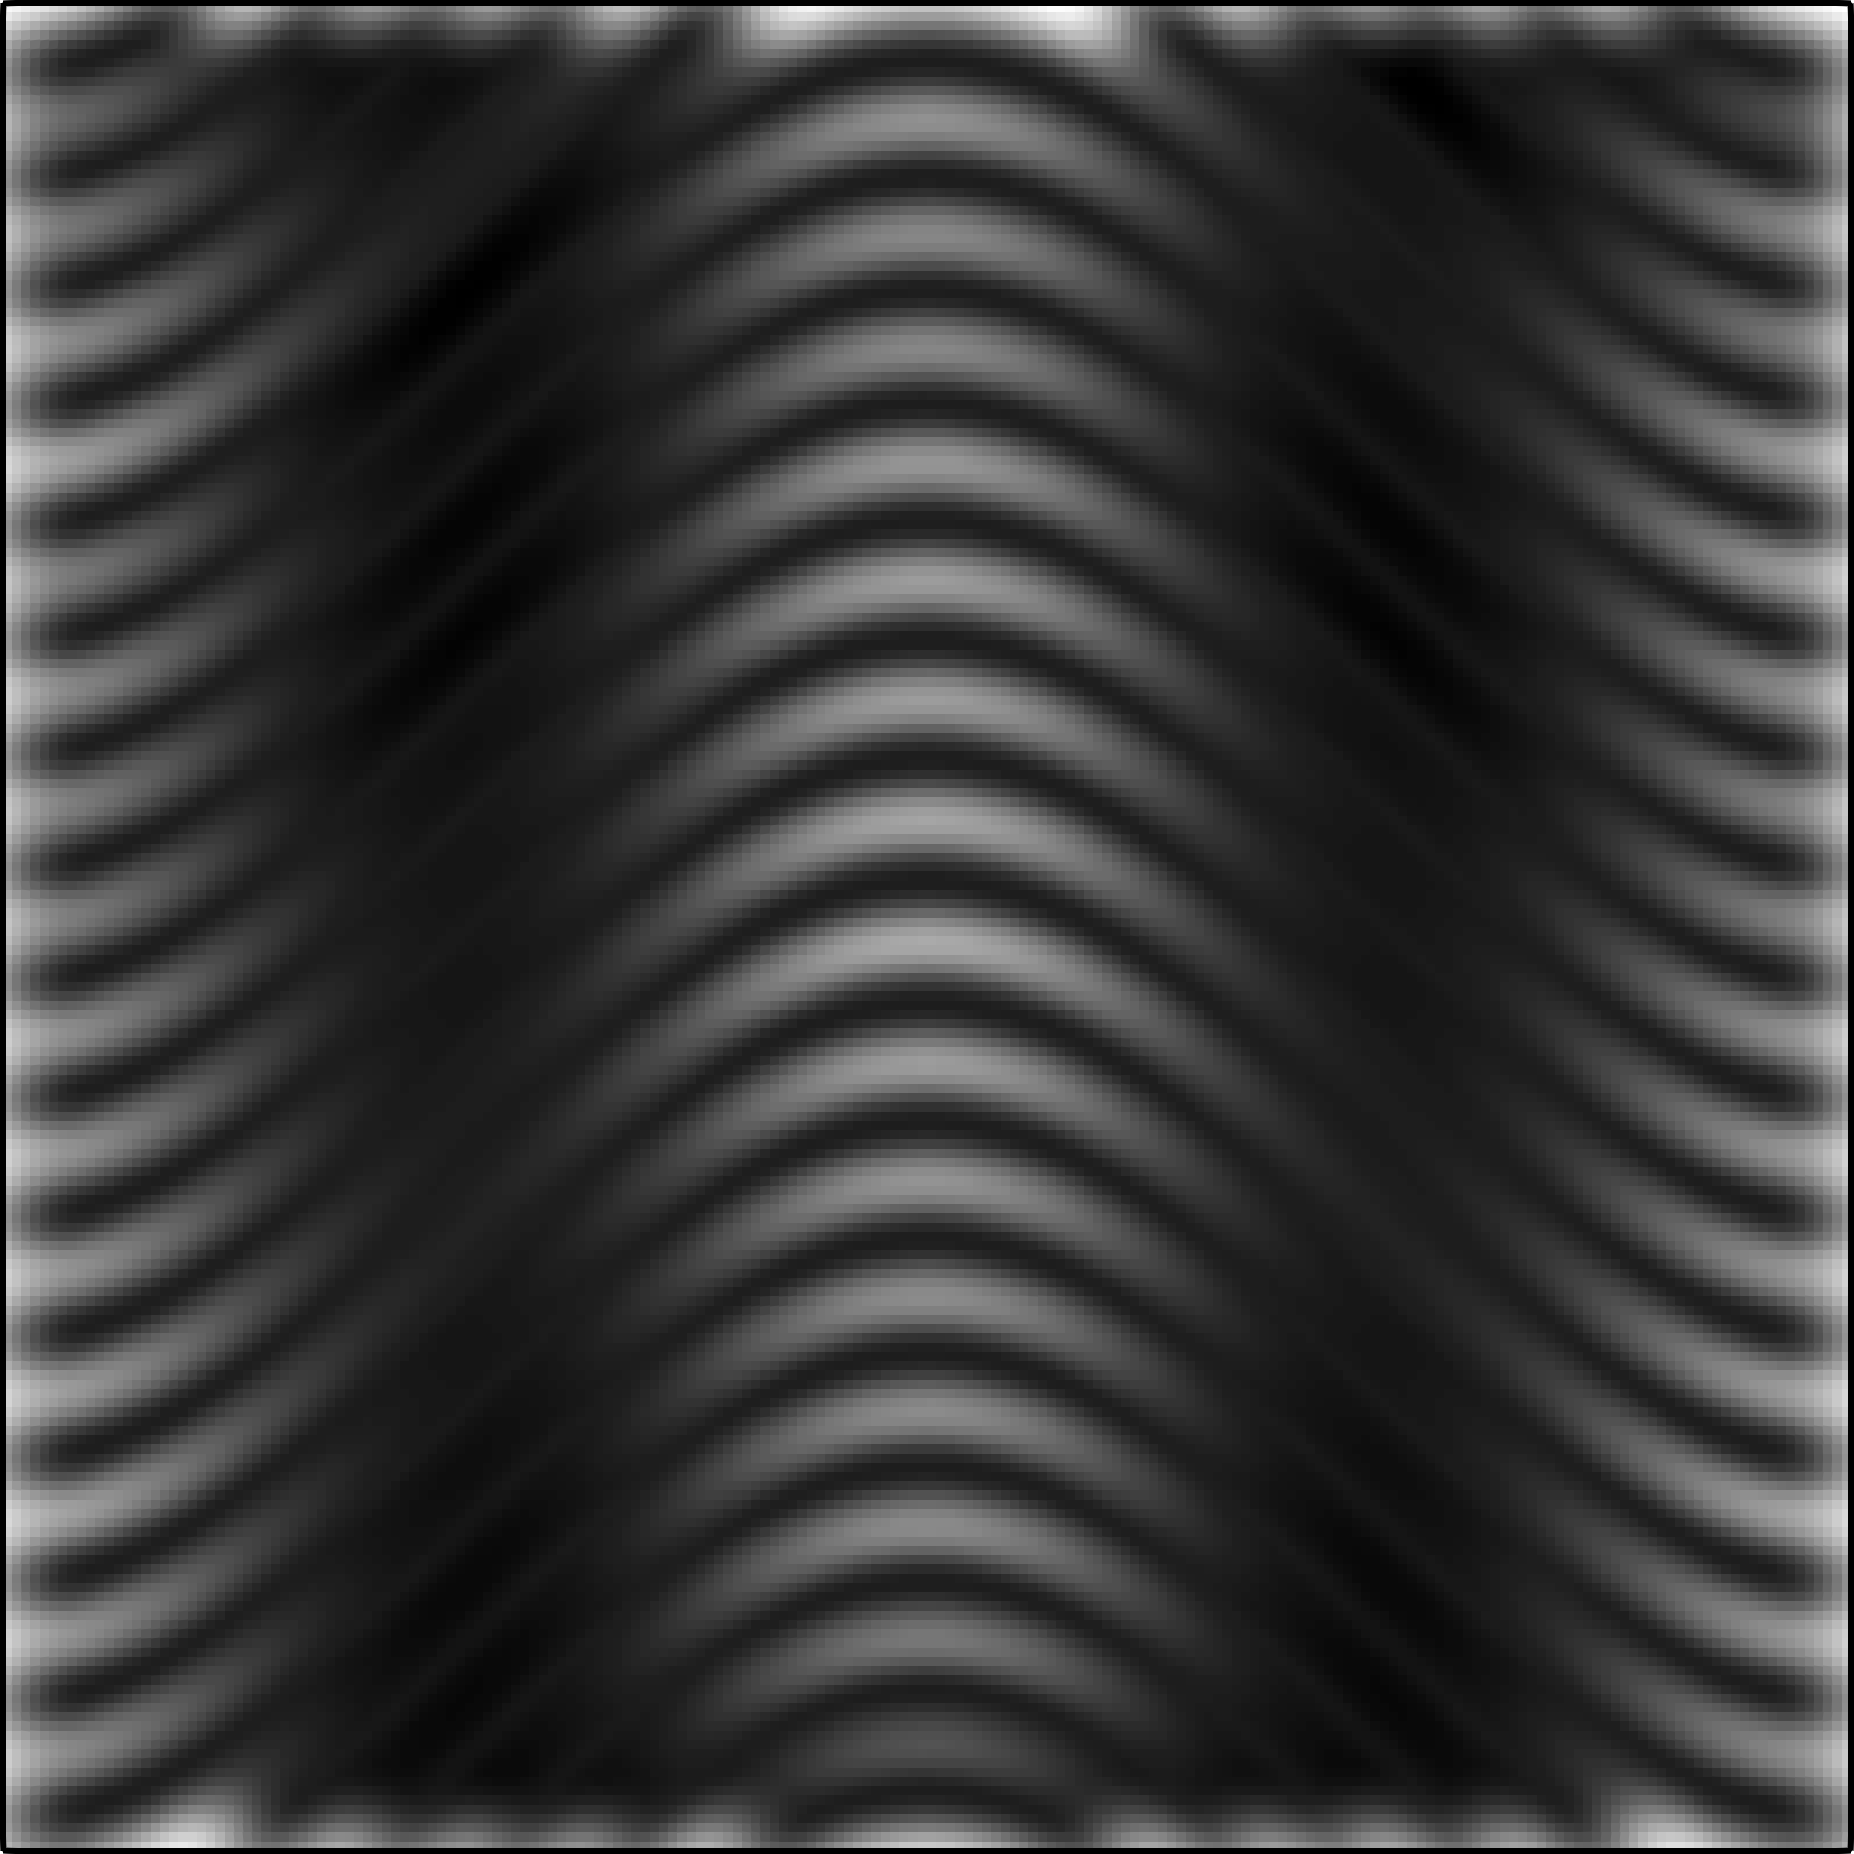
\includegraphics[scale=.08]{figures/WavesStreamlinesBlur.png}
        \caption*{(b)}
    \end{subfigure}
    \begin{subfigure}{.3\textwidth}
        \centering
        \setlength\pgfplotswidth{1.5\textwidth}
        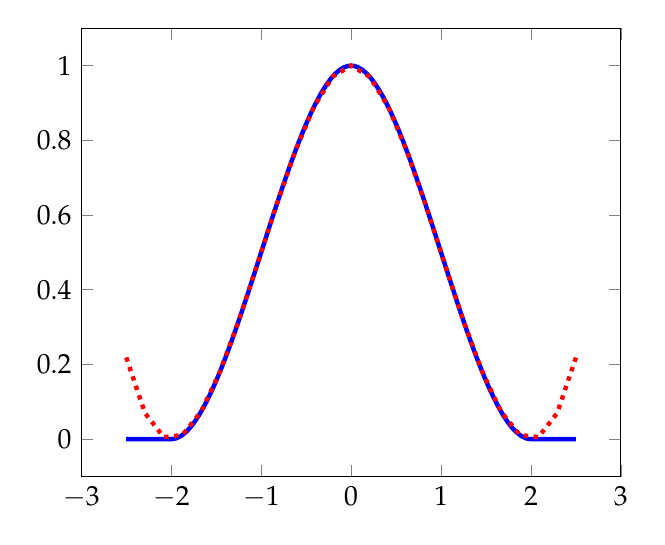
\begin{tikzpicture}
    \def\r(#1){abs(#1) / 2}%
    \begin{axis}
        \addplot[color=blue, ultra thick, samples=100, domain=-2.5:2.5]{
            \r(x) < 1 ? 2*(\r(x))^3-3*(\r(x))^2+1 : 0
        };
        \addplot[color=red, dotted, ultra thick, domain=-2.5:2.5]{
            2*(\r(x))^3-3*(\r(x))^2+1
        };
    \end{axis}
\end{tikzpicture}
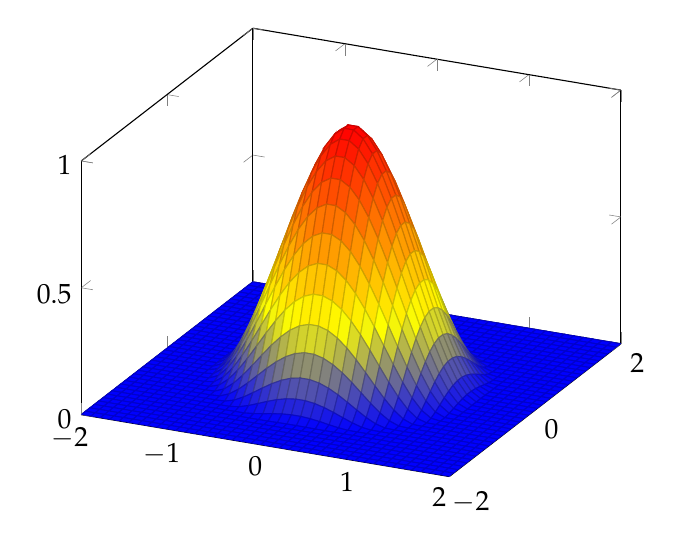
\begin{tikzpicture}[]
    \def\r(#1,#2){(((#1)^2 + (#2)^2) / 2)^0.5}%
    \def\K(#1,#2){2 * \r(#1,#2)^3 - 3 * \r(#1,#2)^2 + 1}
    \begin{axis}[
        % xmin=-2.5,xmax=2,
        % ymin=-2.5,ymax=2,
        zmin= 0  ,zmax=1,
        % axis line style={draw=none},
        % axis equal image,
    ]
    \addplot3[
        surf,
        domain=-2:2,
        samples=40
    ]
    % K(x,y) = 2r^3 - 3r^2 + 1 if r < 1 else 0
    % r = sqrt(x^2 + y^2) / R
    % R = desired radius, lets use 2
    % therefore we get:
    % r = sqrt(x^2 + y^2) / 2
    % K(x,y) = sqrt(x^2 + y^2) / 2 < 1 ? 2 * (sqrt(x^2 + y^2) / 2) ^ 3 - 3 * (sqrt(x^2 + y^2) / 2) ^ 2 + 1 : 0
    {\r(x,y) < 1 ? \K(x,y) : 0};% < 1 ? 2 * r(x,y) ^ 3 - 3 * r(x,y) ^ 2 + 1 : 0};
    \end{axis}
\end{tikzpicture}

        \caption*{(c)}
    \end{subfigure}
    \caption{A set of streamlines (a) generated for the field in \Cref{fig:fundamentals_1}(a). (b) Low-pass version of the image after convolving it with the kernel shown in (c).}
    \label[figure]{fig:fundamentals_2}
\end{figure}
\paragraph*{Spatial Coherence}
    If we want to visualize a vector field, we want its features to be easily identifiable.
    At the same time, we do not want to introduce distractions or artifacts due to the visualization technique.
    The deciding factors of uniformity in streamline visualization are streamline length and density.
    Longer streamlines make for a smoother appearance, whereas many short lines tend to obfuscate and hinder the recognition of important features like the aforementioned critical points.
    Strong spatial coherence is shown in \Cref{fig:fundamentals_2}(a).

\section{Image processing}
\label[section]{sec:IP}
\paragraph{Convolution} A process often found in image- or signal processing.
A kernel (\Cref{fig:fundamentals_1}(c)) is applied to every pixel in an image,
affecting it and other surrounding pixels by adding or subtracting its value at that position. 

\paragraph{Blurring} A special type of convolution, making edges in an image less sharp.
Note the difference between black and white contrast for \Cref{fig:fundamentals_2}(a) and (b).

\section{Roots of Unity}
\label[section]{sec:ROU}
\begin{figure}[ht]
    \centering
    \begin{subfigure}[position]{.5\textwidth}
        \centering
        \setlength\pgfplotswidth{.9\textwidth}
        \begin{tikzpicture}
    \tikzset{
        pics/carc/.style args={#1:#2:#3}{
            code={
               \draw[pic actions] (#1:#3) arc(#1:#2:#3);
            }
        }
    }
    \begin{axis}[ 
        ticks=none,
        axis lines = middle,
        axis line style={->},
        ymin=-1.3, ymax=1.3,
        xmin=-1.3, xmax=1.3,
        xlabel={$1$},
        ylabel={$i$},
        width=\pgfplotswidth,
        height=\pgfplotswidth
        ]
        \draw (0,0) circle [radius=1, fill=white];
        \draw[very thick] (0,0) pic[red]{carc=0:72:2cm};
        \node[red] at (1,1) {$\frac{2\pi}{5}$};

        \draw[very thick, ->] (0,0) -- (1,0) node[midway, above right] {$n_0$};
        \draw[very thick, ->] (0,0) -- ( .309, .951) node[midway, right] {$n_1$};
        \draw[very thick, ->] (0,0) -- (-.809, .588) node[midway, above] {$n_2$};
        \draw[very thick, ->] (0,0) -- (-.809,-.588) node[midway, below] {$n_3$};
        \draw[very thick, ->] (0,0) -- ( .309,-.951) node[midway, right] {$n_4$};
    \end{axis}
\end{tikzpicture}

        \caption*{(a)}
    \end{subfigure}
    \caption*{The 5th roots of unity $n_0...n_4$ partition the unit circle equally}
\end{figure}
With $i$ being the complex number, we can use Euler's equation \[n_j = e^{ji2\pi/k}, j = 0, 1, ..., k-1\] to obtain $k$ numbers lying on the complex unit circle,
which are called the $k$-th roots of unity.
Notable properties are their length of exactly one, and that they divide the unit circle equally.
We can convert them to vectors in $\mathbb{R}^2$ using \[\vec{v_j} = (\operatorname{Re}(n_j), \operatorname{Im}(n_j))^T\]

% paar mehr beispiele, convolution etc, ausblick
% which algortimh?
  \chapter{Method}
\section{Failed Attempt}
\begin{leftbar}
    \noindent
    At first, it was attempted to create a custom algorithm capable of streamline placement in 3D.
    We then wanted to introduce changes that allowed the lines to be placed adhering to spatial coherence.
    Unfortunately, this was met with failure relatively quickly.
    The algorithm proposed was simply too greedy, and did not yield good initial results.
    Adding time coherence in this case would be of very little benefit here, since the initial image quality and performance degraded way too quickly for it to be actually useful.
    We still outline some of it in this chapter, in case it is of interest or as an example.
\end{leftbar}
\noindent
We start with a simple algorithm to generate streamlines in a 2D slice of a vector field.
The local z-component of the Cartesian grid is simply set to zero for the relevant sections of the algorithm.
The algorithm uses two operations: Streamline Traversal and Seed Filtering, which are executed round-robin.
\subsection{Streamline Traversal}
The Streamline Traversal process works as follows:
\begin{itemize}
    \begin{minipage}{.6\textwidth}
    \item \textbf{Step 1:}
    Choose a seed point from a list of candidates (initially an arbitrary point from the dataset) and remove it from the list.
    Then integrate forward and backward to obtain the other points on the streamline, until
    a number of steps is reached, we cross the bounding box, or we get too close to another streamline.
    \item \textbf{Step 2:}
    Compute the normals, add and subtract them to the succeeding point. The first point (according to step count in backward iteration) will not have a preceding normal, and is not used in this step. These points are new seed candidates for further streamline placement.
    \end{minipage}
    \begin{minipage}{.3\textwidth}
    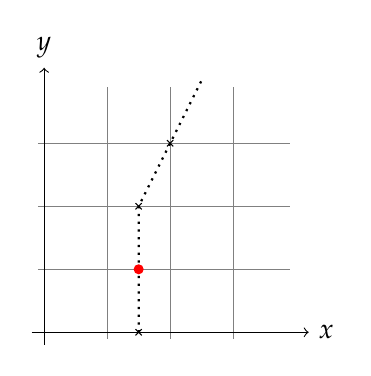
\begin{tikzpicture}[domain=0:4, scale=.8]
    \draw[very thin,color=gray] (-0.1,-0.1) grid (3.9,3.9);

    \draw[->] (-0.2,0) -- (4.2,0) node[right] {$x$};
    \draw[->] (0,-0.2) -- (0,4.2) node[above] {$y$};

    \draw[dotted, thick] (1.5,0) -- (1.5,2) -- (2.5,4);

    \draw[red] plot[only marks, mark=*] coordinates{(1.5,1)};
    \draw plot[only marks, mark=x] coordinates{(1.5,0) (1.5,2) (2,3)};
\end{tikzpicture}

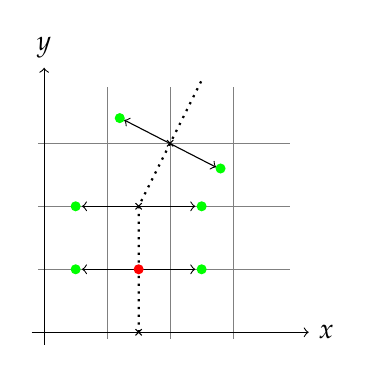
\begin{tikzpicture}[domain=0:4, scale=.8]
    \draw[very thin,color=gray] (-0.1,-0.1) grid (3.9,3.9);
    
    \draw[->] (-0.2,0) -- (4.2,0) node[right] {$x$};
    \draw[->] (0,-0.2) -- (0,4.2) node[above] {$y$};

    \draw[<->] (0.6, 1) -- (2.4, 1);
    \draw[<->] (0.6, 2) -- (2.4, 2);
    \draw[<->] (1.27, 3.37) -- (2.73, 2.62);
    
    \draw[dotted, thick] (1.5,0) -- (1.5,2) -- (2.5,4);
    
    \draw[red] plot[only marks, mark=*] coordinates{(1.5,1)};
    \draw plot[only marks, mark=x] coordinates{(1.5,0) (1.5,2) (2,3)};
    \draw[green] plot[only marks, mark=*] coordinates{(0.5,1) (2.5, 1) (0.5, 2) (2.5, 2) (1.2,3.4) (2.8, 2.6)};
    
\end{tikzpicture}



% \begin{tikzpicture}[domain=0:4]
%   \draw[very thin,color=gray] (-0.1,-0.1) grid (3.9,3.9);

%   \draw[->] (-0.2,0) -- (4.2,0) node[right] {$x$};
%   \draw[->] (0,-0.2) -- (0,4.2) node[above] {$y$};
%   \draw plot[only marks, mark=*] coordinates{(1,1)};
%   \draw[color=red]    plot (\x,\x)             node[right] {$f(x) =x$};
%   % \x r means to convert '\x' from degrees to _r_adians:
%   \draw[color=blue]   plot (\x,{sin(\x r)})    node[right] {$f(x) = \sin x$};
%   \draw[color=orange] plot (\x,{0.05*exp(\x)}) node[right] {$f(x) = \frac{1}{20} \mathrm e^x$};
% \end{tikzpicture}


    \end{minipage}
\end{itemize}
\subsection{Seed Filtering}
Since after the 1st iteration, roughly half of the points added by step 2 will be very close to the preceding iteration's points, we store the parent's points and remove any new points from the current step if they are too close to the parent's points.
Furthermore, a grid is used to track the global state of the field w.r.t to lines existing in individual segments.
This is used to determine whether a line is getting too close to another or if it has room to expand. Streamlines are removed if their length is shorter than 10 iteration steps.
\section{Steady Field Streamline Placement in 3D}
Instead of the trivial normal(s), we now use a normal plane around the streamline trajectory, created via numpy's QR-decomposition. The algorithm returns orthonormalized vectors, the first column vector's direction being equal to the first provided input vector.
We can therefore feed it the streamline trajectory and two basis vectors, and receive 2 orthonormal basis vectors $b_0, b_1$.\\
With $i$ being the complex number, we obtain $k$ roots of unity via \[n_j = e^{ji2\pi/k}, j = 0, 1, ..., k-1\]
We then transform them into our 3D frame of reference using \[v_i = re(n_i)*b_0 + im(n_i)*b_1 \] This gives us $k$ uniformly placed  vectors in the normal plane around the current streamline segment. The rest of the algorithm stays largely the same, the grid is simply extended into the 3rd dimension.
\newpage

\section{The Image-Guided Algorithm by Turk and Banks}
\label[section]{sec:basealg}
\begin{figure}[ht]
    \centering
    \begin{subfigure}{.49\textwidth}
        \centering
        \includegraphics*[scale=.09]{figures/TBWaves1.png}
        \caption*{(a)}
    \end{subfigure}
    \begin{subfigure}{.49\textwidth}
        \centering
        \includegraphics*[scale=.09]{figures/TBWaves2.png}
        \caption*{(b)}
    \end{subfigure}
    \caption{
        (a) Short streamlines placed with seeds on a regular grid.
        (b) Same streamlines after optimization through seed shifting. Notice the more even grayscale image in the center and on the sides.
        Both images contain 130 streamlines, with a length of 10\,\% of the screen width each.}
    \label[figure]{fig:tbwaves}
\end{figure}

In this chapter, we introduce the image-guided streamline placement
algorithm developed by Greg Turk and David Banks \cite{TurkBanks}.
The algorithm forms a more suitable basis for time coherence due to how it reacts to changes to single streamlines.
It retains a good amount of control regarding the streamline placement and length,
while still allowing the streamlines to move and relax the spacing between them.

\subsection{Overview}
The following section will be about the three core components that make up the image-guided
sections of the algorithm: the streamlines themselves, the low-pass filter, and the energy measure.
The filter creates blurred images of the streamlines,
where pixels close to the streamline are brighter, and empty spaces darker (\Cref{fig:tbwaves}(a)).
An optimal streamline placement w.r.t. density (neither too crowded, nor too sparse)
is reached when the low-pass image has roughly the same gray coloring everywhere.
We can intuitively define the energy measure as the squared differences of the blurred image from
a uniform grayscale background, also referred to as the \textit{target brightness}.
Simply knowing the energy however is not enough, we need to be able to manipulate
the streamline placement effectively in order to minimize it.
This is achieved using various randomized changes to the position (\Cref{fig:tbwaves}(b)), length,
or number of streamlines, and is described in greater detail in \Cref{sec:tbmove}.
Whenever a change leads to a decrease in energy, the change is accepted and, if not, reverted.

\subsection{Energy Measure}
The method used by Turk and Banks defines three important components to measure image quality as the
sum of deviations of a low-pass blurred image (fundamentals, \Cref{sec:IP}) from a uniform grayscale target.
\begin{enumerate}
    \item The first component is a collection of straight line segments from each streamline,
    each of which are converted to a line formula of the form $Ax + By - C = 0$.
    They refer to the image defined by these purely analytical line segments as $I$,
    however this image is never actually created and exists purely implicitly.
    \begin{equation*}
        I(x,y) = \begin{cases}
            1, \kern4em & \text{pixel lies on streamline}\\
            0,          & \text{else}
    \end{cases}
    \end{equation*}
    
    \item The second component is the low-pass filter $L$.
    It uses a kernel to generate the filtered image of a streamline.
    Given a falloff distance $R$ and $r=\sqrt{x^2+y^2} / R$, the kernel is defined as:
    \begin{equation*}
        K(x,y) = \begin{cases}
            2r^3 - 3r^2 + 1, \kern4em & r < 1\\
            0,               & r >= 1
        \end{cases}
    \end{equation*}
    Every pixel within the bounding box of a segment + filter diameter has its brightness altered according to this kernel.
    Due to the implementation of the convolution and the scaling of the filter brightness, it is guaranteed that every pixel reaches a maximum brightness of 1.
    This is invariant w.r.t. the number or length of segments as long as only a single,
    straight streamline section is considered.
    Conversely, the only way to get a brightness greater than one is either via a curve in the streamline or
    two streamlines being too close to each other.
    This is immensely useful, as it allows two streamlines to get close to each other from the ends, 
    but not from the sides (\Cref{fig:tbwaves}(b)).
    
    \item In order to determine the brightness, also referred to as the \textit{energy}
    of the image generated by the kernel application,
    the following expression is used as the \textit{energy function}:
    \begin{equation}
        E(I) = \int_x\int_y\left[(L\ast I)(x,y)-t\right]^2\,\text{d}x\,\text{d}y
    \end{equation}
    With $t$ referring to the \textit{target brightness}, in their source code the number one is used.
\end{enumerate}
It is pivotal for this energy measure to react to minimal changes for the algorithm to successfully converge.
Therefore, this algorithm does \textit{not} use a simple rasterization and blur technique,
as the initial discretization/rasterization
of the streamline would remove too much information, even when using anti-aliasing or
other more sophisticated rasterization techniques like Bresenham's line algorithm.
While we discuss the actual implementation in chapter 5, the takeaway here is that the streamline
remains in its analytical form as segments between points.
Then, every point inside the bounding box around every line segment calculates its brightness
based on the line equation, not by simply blurring pixels on the streamline, leading to much higher sensitivity.

\subsection{Randomized Optimizations}
\label[section]{sec:tbmove}
Turk and Banks define six actions:
\begin{itemize}
    \item \textbf{Insert, Delete:} Add or remove a streamline from the image.
    \item \textbf{Lengthen, Shorten:} In-/Decrease the length of a streamline on one or both ends.
    \item \textbf{Combine:} Join two streamlines head-to-tail.
    \item \textbf{Move:} Translate the seed of a streamline by a small distance.
\end{itemize}
These actions are selected randomly with random parameters, then applied to a random streamline.
The algorithm terminates after an energy range was reached, or accepted changes become rare enough to not introduce changes anymore.\\
If the change was deemed beneficial according to a decrease in energy, it is accepted, otherwise the changes are reverted.
This causes a "drift" of the streamlines toward a more uniform energy level.
Naturally, this depends heavily on the choice of $t$. If $t$ were to be chosen closer to two,
the image would become crowded by many streamlines to reach the increased target gray level.
\newpage


\section{Why Time Coherence is Necessary}


\begin{figure}[ht!]
    \centering
    \begin{subfigure}{.3\textwidth}
        \centering
        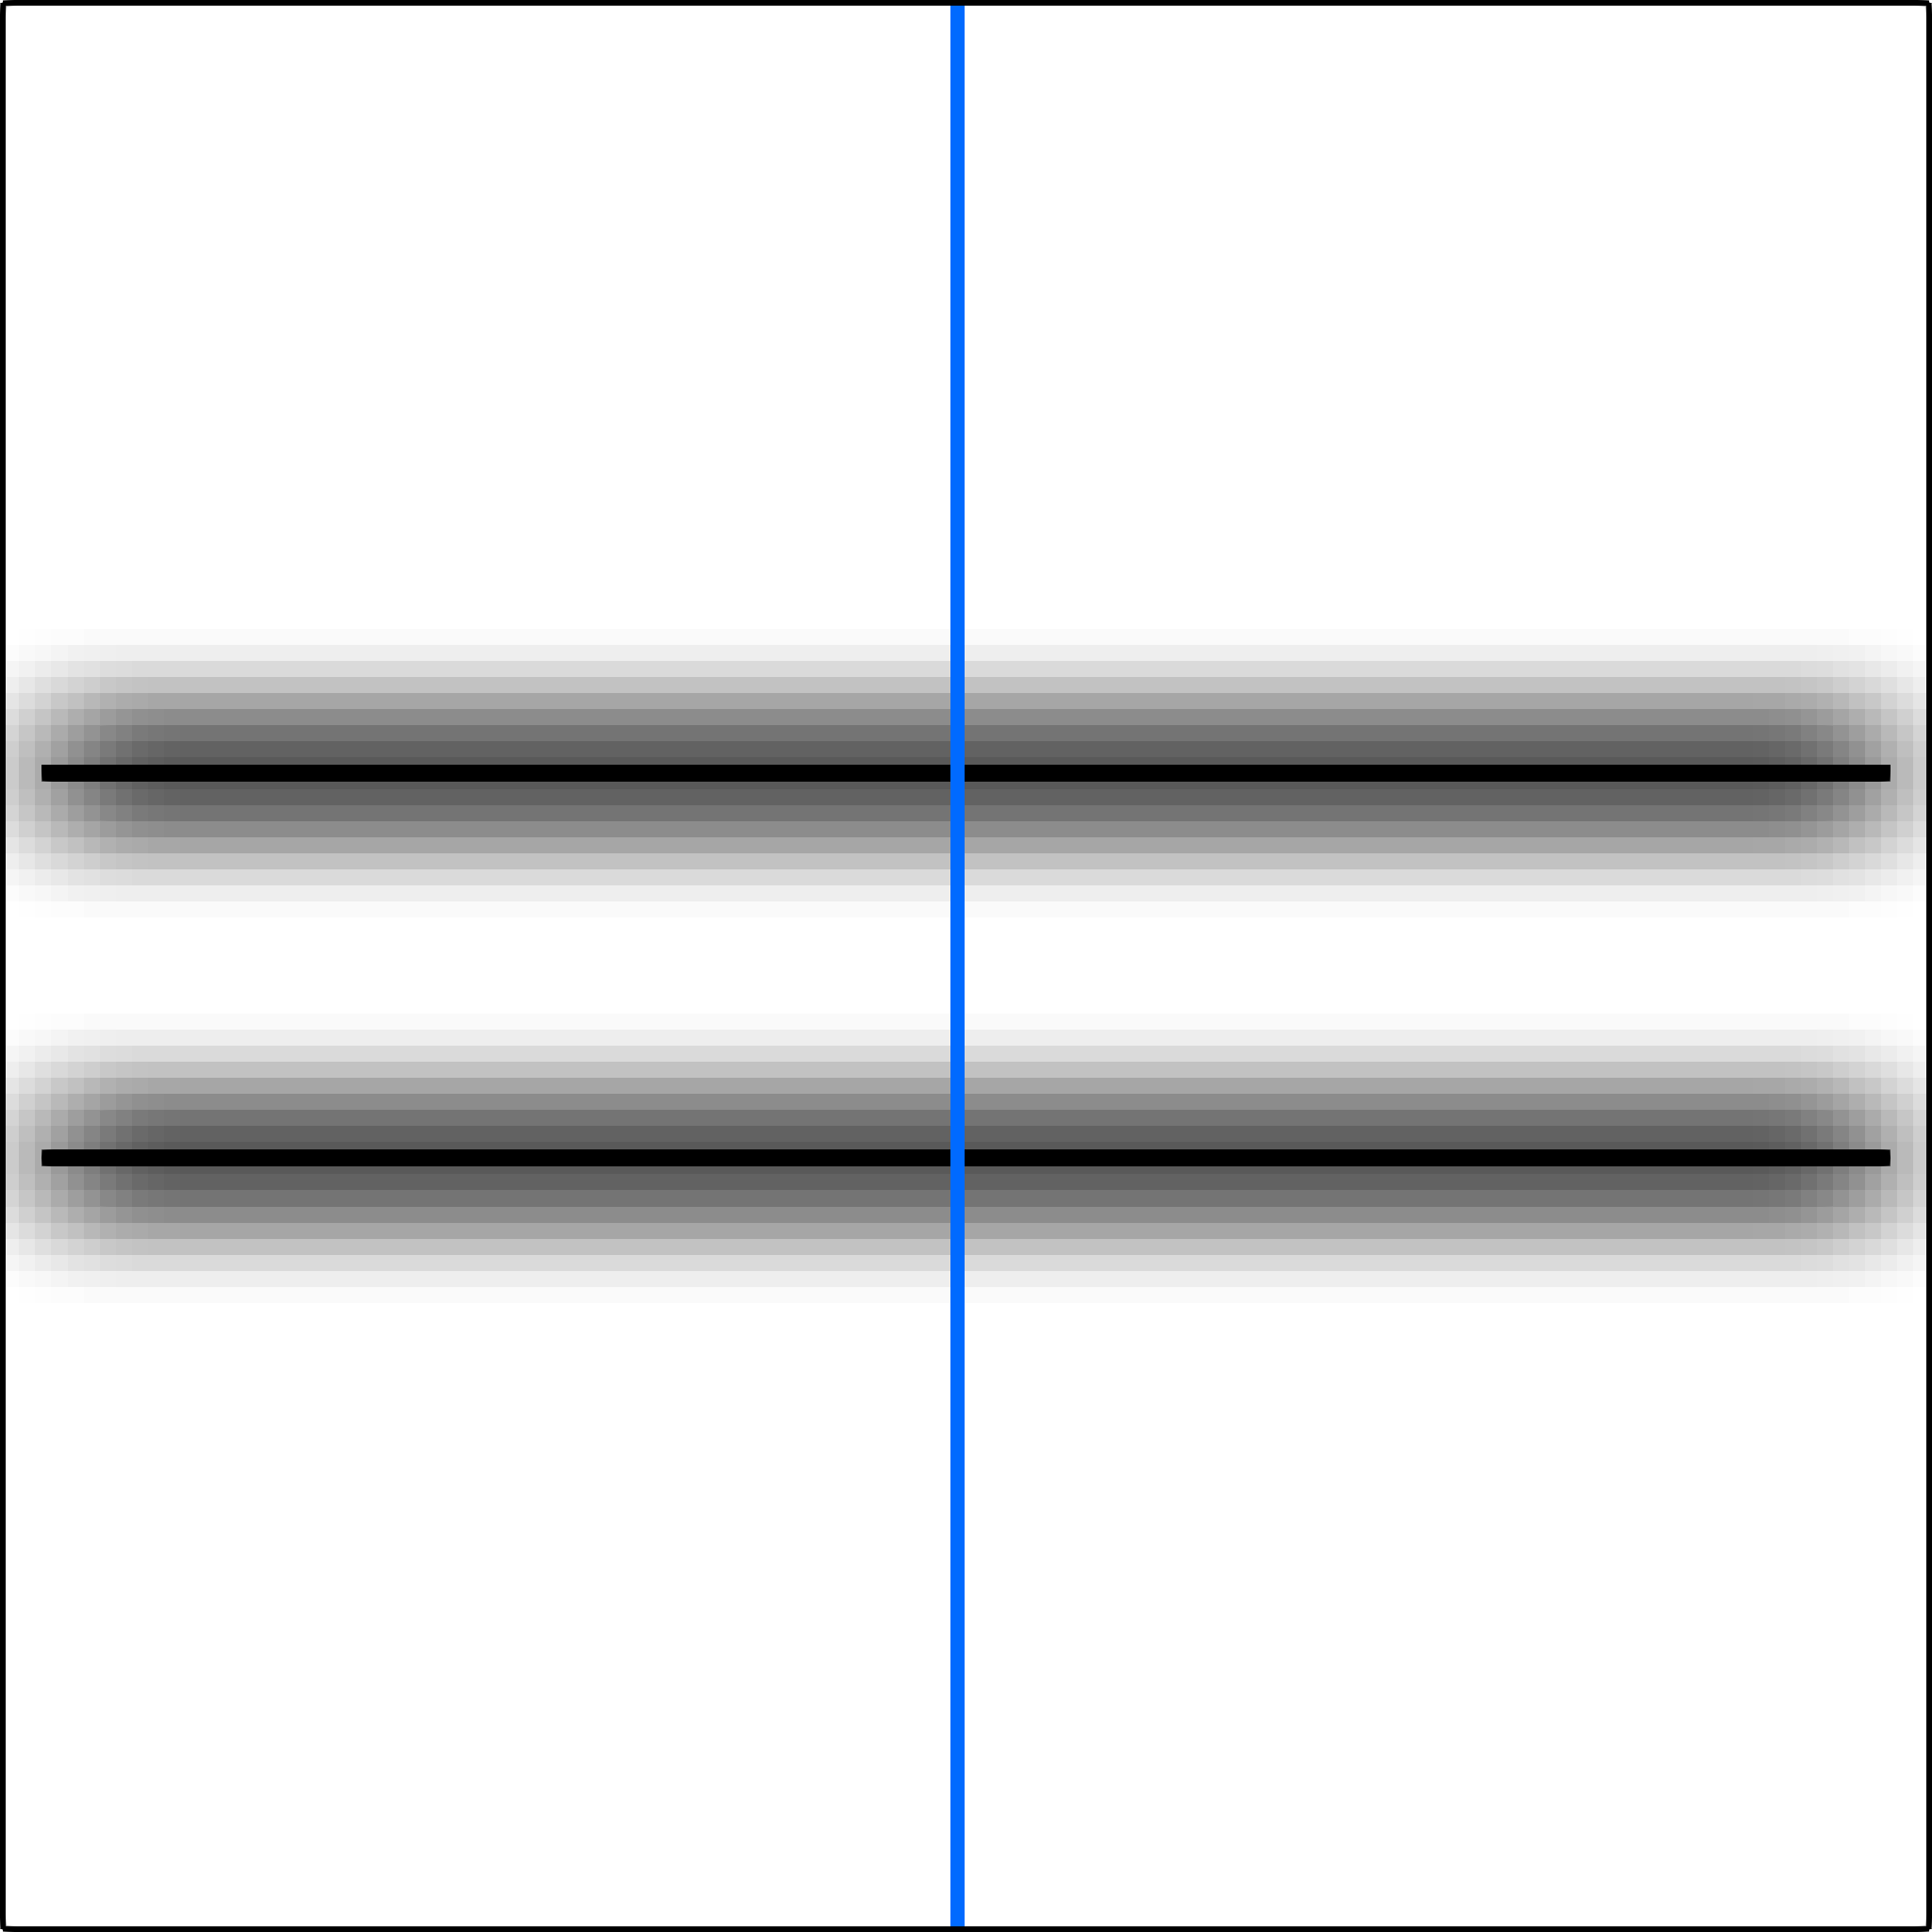
\includegraphics[scale=.075]{figures/FilterRadius/Distant.png}
        \caption*{(a)}
    \end{subfigure}
    \begin{subfigure}{.3\textwidth}
        \centering
        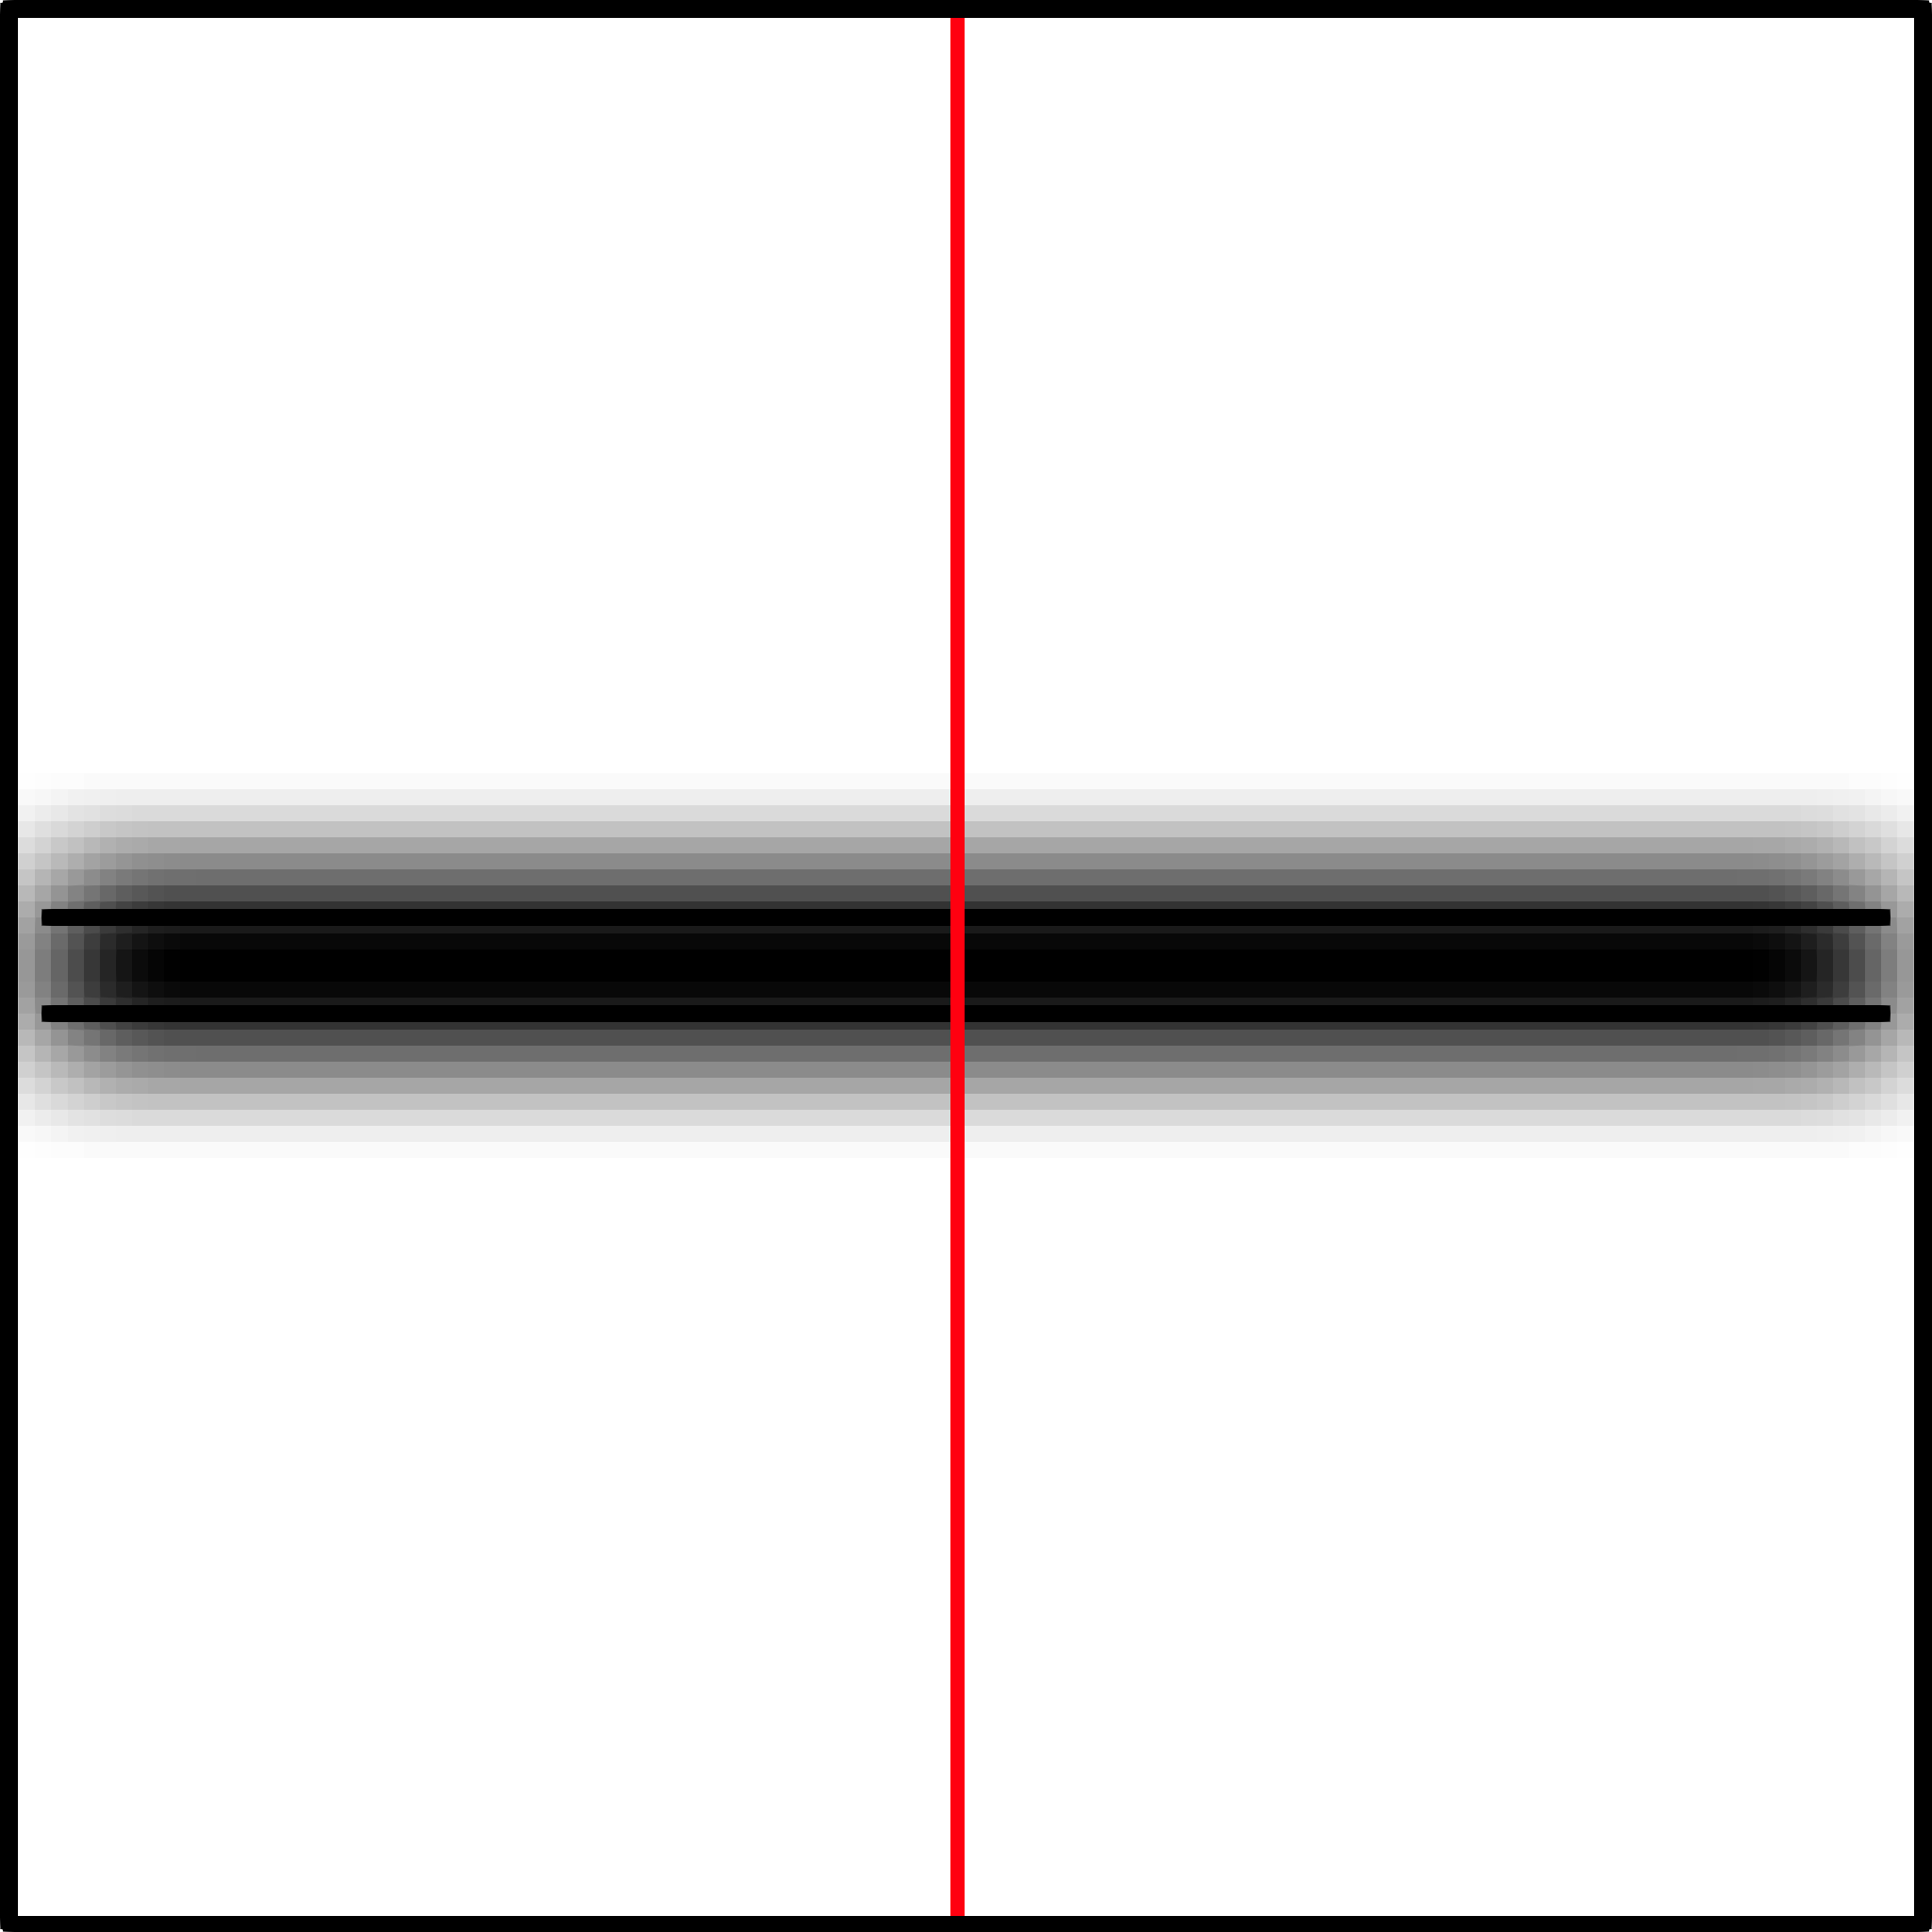
\includegraphics[scale=.075]{figures/FilterRadius/Close.png}
        \caption*{(b)}
    \end{subfigure}
    \begin{subfigure}{.375\textwidth}
        \centering
        \resizebox{\textwidth}{!}{
            % Data for the first, distant pair of horizontal lines. Extracted along the y axis via target.data[20, :].round(3)

% [0.   0.   0.   0.   0.   0.   0.   0.   0.   0.   0.   0.   0.   0.
%  0.   0.   0.   0.   0.   0.   0.   0.   0.   0.   0.   0.   0.   0.
%  0.   0.   0.   0.   0.   0.   0.   0.   0.   0.   0.   0.04 0.11 0.23
%  0.38 0.55 0.71 0.86 0.97 1.03 1.03 0.97 0.86 0.71 0.55 0.38 0.23 0.11
%  0.04 0.   0.   0.   0.   0.   0.   0.04 0.11 0.23 0.38 0.55 0.71 0.86
%  0.97 1.03 1.03 0.97 0.86 0.71 0.55 0.38 0.23 0.11 0.04 0.   0.   0.
%  0.   0.   0.   0.   0.   0.   0.   0.   0.   0.   0.   0.   0.   0.
%  0.   0.   0.   0.   0.   0.   0.   0.   0.   0.   0.   0.   0.   0.
%  0.   0.   0.   0.   0.   0.   0.   0.  ]


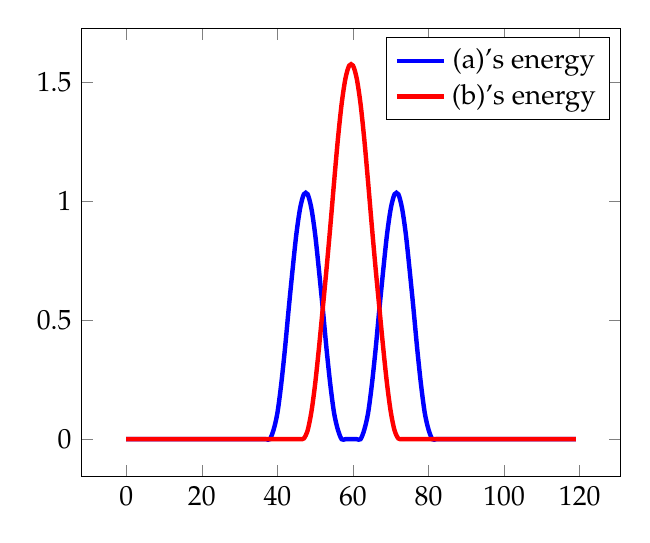
\begin{tikzpicture}
    \begin{axis} [every axis plot post/.append style={ultra thick, mark=none}, xlabel=]
        \addplot +[smooth] [color=blue] coordinates {
            (0, 0.)
            (1, 0.)
            (2, 0.)
            (3, 0.)
            (4, 0.)
            (5, 0.)
            (6, 0.)
            (7, 0.)
            (8, 0.)
            (9, 0.)
            (10, 0.)
            (11, 0.)
            (12, 0.)
            (13, 0.)
            (14, 0.)
            (15, 0.)
            (16, 0.)
            (17, 0.)
            (18, 0.)
            (19, 0.)
            (20, 0.)
            (21, 0.)
            (22, 0.)
            (23, 0.)
            (24, 0.)
            (25, 0.)
            (26, 0.)
            (27, 0.)
            (28, 0.)
            (29, 0.)
            (30, 0.)
            (31, 0.)
            (32, 0.)
            (33, 0.)
            (34, 0.)
            (35, 0.)
            (36, 0.)
            (37, 0.)
            (38, 0.)
            (39, 0.04)
            (40, 0.11)
            (41, 0.23)
            (42, 0.38)
            (43, 0.55)
            (44, 0.71)
            (45, 0.86)
            (46, 0.97)
            (47, 1.03)
            (48, 1.03)
            (49, 0.97)
            (50, 0.86)
            (51, 0.71)
            (52, 0.55)
            (53, 0.38)
            (54, 0.23)
            (55, 0.11)
            (56, 0.04)
            (57, 0.)
            (58, 0.)
            (59, 0.)
            (60, 0.)
            (61, 0.)
            (62, 0.)
            (63, 0.04)
            (64, 0.11)
            (65, 0.23)
            (66, 0.38)
            (67, 0.55)
            (68, 0.71)
            (69, 0.86)
            (70, 0.97)
            (71, 1.03)
            (72, 1.03)
            (73, 0.97)
            (74, 0.86)
            (75, 0.71)
            (76, 0.55)
            (77, 0.38)
            (78, 0.23)
            (79, 0.11)
            (80, 0.04)
            (81, 0.)
            (82, 0.)
            (83, 0.)
            (84, 0.)
            (85, 0.)
            (86, 0.)
            (87, 0.)
            (88, 0.)
            (89, 0.)
            (90, 0.)
            (91, 0.)
            (92, 0.)
            (93, 0.)
            (94, 0.)
            (95, 0.)
            (96, 0.)
            (97, 0.)
            (98, 0.)
            (99, 0.)
            (100, 0.)
            (101, 0.)
            (102, 0.)
            (103, 0.)
            (104, 0.)
            (105, 0.)
            (106, 0.)
            (107, 0.)
            (108, 0.)
            (109, 0.)
            (110, 0.)
            (111, 0.)
            (112, 0.)
            (113, 0.)
            (114, 0.)
            (115, 0.)
            (116, 0.)
            (117, 0.)
            (118, 0.)
            (119, 0.)
        };
        \addplot +[smooth] [color=red] coordinates {
            (0, 0.)
            (1, 0.)
            (2, 0.)
            (3, 0.)
            (4, 0.)
            (5, 0.)
            (6, 0.)
            (7, 0.)
            (8, 0.)
            (9, 0.)
            (10, 0.)
            (11, 0.)
            (12, 0.)
            (13, 0.)
            (14, 0.)
            (15, 0.)
            (16, 0.)
            (17, 0.)
            (18, 0.)
            (19, 0.)
            (20, 0.)
            (21, 0.)
            (22, 0.)
            (23, 0.)
            (24, 0.)
            (25, 0.)
            (26, 0.)
            (27, 0.)
            (28, 0.)
            (29, 0.)
            (30, 0.)
            (31, 0.)
            (32, 0.)
            (33, 0.)
            (34, 0.)
            (35, 0.)
            (36, 0.)
            (37, 0.)
            (38, 0.)
            (39, 0.)
            (40, 0.)
            (41, 0.)
            (42, 0.)
            (43, 0.)
            (44, 0.)
            (45, 0.)
            (46, 0.)
            (47, 0.003)
            (48, 0.037)
            (49, 0.115)
            (50, 0.234)
            (51, 0.384)
            (52, 0.549)
            (53, 0.716)
            (54, 0.894)
            (55, 1.081)
            (56, 1.26)
            (57, 1.41)
            (58, 1.516)
            (59, 1.571)
            (60, 1.571)
            (61, 1.516)
            (62, 1.41)
            (63, 1.26)
            (64, 1.081)
            (65, 0.894)
            (66, 0.716)
            (67, 0.549)
            (68, 0.384)
            (69, 0.234)
            (70, 0.115)
            (71, 0.037)
            (72, 0.003)
            (73, 0.)
            (74, 0.)
            (75, 0.)
            (76, 0.)
            (77, 0.)
            (78, 0.)
            (79, 0.)
            (80, 0.)
            (81, 0.)
            (82, 0.)
            (83, 0.)
            (84, 0.)
            (85, 0.)
            (86, 0.)
            (87, 0.)
            (88, 0.)
            (89, 0.)
            (90, 0.)
            (91, 0.)
            (92, 0.)
            (93, 0.)
            (94, 0.)
            (95, 0.)
            (96, 0.)
            (97, 0.)
            (98, 0.)
            (99, 0.)
            (100, 0.)
            (101, 0.)
            (102, 0.)
            (103, 0.)
            (104, 0.)
            (105, 0.)
            (106, 0.)
            (107, 0.)
            (108, 0.)
            (109, 0.)
            (110, 0.)
            (111, 0.)
            (112, 0.)
            (113, 0.)
            (114, 0.)
            (115, 0.)
            (116, 0.)
            (117, 0.)
            (118, 0.)
            (119, 0.)
        };
        \addlegendentry{(a)'s energy}
        \addlegendentry{(b)'s energy}
    \end{axis}
\end{tikzpicture}
        }
        \caption*{(c)}
    \end{subfigure}
    \caption{
        How the proximity of streamlines changes the brightness of their respective footprints in a 120x120\,px image.
        (a) Two streamlines approx. three times the blur radius apart.
        (b) Two streamlines only 3/4 the blur radius apart.
        (c) Energy of the more distant streamlines (a, blue) and the closer ones (b, red) is shown in the $y$-axis.
        The $x$-axis shows the height of the pixels taken along the red and blue
        strips in (a) and (b) respectively, counted from the top.
    }
    \label[figure]{fig:closeenergy}
\end{figure}
\section{Time Coherence - Definition}
\label[section]{sec:tcdef}
Based on the desired image overlap and concepts from computing the energy measure, we can infer a measure for time coherence.
We base this measure on the spatial energy function $E$ from the Turk and Banks algorithm.
\begin{leftbar}
    \textbf{Notation:} To avoid confusion, we from now on write the spatial components (former $E$ and $L$)
    as $E_s, L_s$ to better separate them from their temporal counterparts $E_t$ and $L_t$.
    $t$ has two further uses:
    If we talk about time steps, $t$ refers to the time, e.g., when describing vector fields $u(x,y,t)$.
    In the context of the Turk and Banks algorithm, $t$ is the target brightness.
\end{leftbar}

Instead of the comparison between a low-pass image of streamlines and a constant target brightness used in $E_s$,
the temporal energy $E_t$ now depends on two sets of streamlines ($I_0, I_1$) and uses a different low-pass filter ($L_t$):
\[E_t(I_0, I_1) = \int_x\int_y\left[(L_t\ast I_0)(x,y)-(L_t\ast I_1)(x,y)\right]^2\,\text{d}x\,\text{d}y\]
This measure tells us the sum of squared difference between the energy of two different sets of streamlines.
Allowing for a new kernel gives us more freedom to change \textit{how} we measure the temporal energy,
as we do not want it to behave the same way as the spatial energy does.
For example, the measure $E_s$ of two neighboring streamlines is the strongest in
the center of them, not at the actual streamline positions, which can be seen in \Cref{fig:closeenergy}.
This means that by using $E_s$ instead of $E_t$,
we would change the number or position of streamlines by drawing them into the center of two former streamlines,
thereby intently worsening time coherence.
Conversely, this would also prohibit streamline creation at darker spots, giving rise to holes in our streamline image.

The optimum for time coherence would of course be two identical sets of streamlines, which effectively minimize $E_t$ to zero.

% Combining it with the spatial measure $E$ via linear interpolation gives us a good amount of control how strong we want the coherence to be.

% Time Coherence refers to how a vector field behaves through different time steps.
% Intuitively, we consider areas within the field to be of high temporal coherence if the lines drawn on them are relatively stationary.
% Vice versa, we can say that an area of high fluctuation will be of low temporal coherence.
% A more formal definition employed in our algorithm is as follows:
% Given a field $F$ and a starting point $S_0$ (called the "seed"), we can integrate over the field.
% This yields a set of points $S^0$ which define a streamline containing every reached point, written as $S^0 = \int(S_0, F)$.
% We can therefore assign a streamline to every point in our field (and vice versa).
% Given $S_0$ and an unsteady field $F(t)$, compute for each time step $t_1...t_n$ the streamline $S^{0,t_i} = \int(S_0, F(t_i))$.
% In order to convert these sets of lines to a scalar, we use the Hausdorff Distance $dist(S^i,S^j)$,
% giving us the greatest minimal distance between any pair of two sets.
% We can therefore create a map $coh(S_i, F(t)): max(dist(\int(S_i, F(t_k)), \int(S_i, F(t_l))))$,
% sending each point in an unsteady vector field to a scalar, and thereby determining its temporal coherence.

\section{Adding Time Coherence}
\label[section]{sec:tcalg}
This section will be about how we translated the definition from section 4.4 into a functional component for our algorithm.
We use the aforementioned energy measure to induce a process we refer to as \textit{coaxing}, as we are applying continued pressure to lines to move them in the direction of their former footprints.

\noindent A second addition called \textit{shattering} will be introduced as well,
where lines are split into smaller segments (\textit{fragments}) to be used as the starting layout in the next timestep.
This can increase coherence as well by seeding lines at the same place, and works especially well in combination with coaxing.

% After introducing a new kernel $L_t$ with roughly half the radius of $L_s$, spots of elevated brightness are now very uncommon.
% They do not affect the line placement in a way noticeable to the naked eye anymore.
% Another benefit is that lines further away than that radius will not be influenced, so that the backfilling of an empty spot is mostly of local consequence.

% After an image has reached its final state, we shatter it, breaking every streamline into a number of smaller streamlines, called \textit{shards}.
% Every line is divided equally into shards of roughly the start length of our lines.
% The shards are then used as our initial seeding pattern instead of the regular grid for the next frame.
% This means that when shattering is enabled, we only generate the initial seeds for the first frame, every subsequent frame gets its initial seeds via the shatter process of the previous one.

\subsection{Coaxing}
Since most of the algorithm's optimization is centered around the comparison with an energy level before and after an action was taken,
modifying the energy function provides a lot of leverage regarding how lines are placed. 
In order to make the algorithm favor previous line positions, we therefore rewrite the energy function as the linear
interpolation between $E_s$ and $E_t$. This gives us good control over how much time coherence we apply, as choosing too much will cause a degradation in image quality.
Given the previous frame's low-pass image with the time kernel $(L_t\ast I_0)$ we use:
\begin{equation*}
    \begin{split}
        E(I_0, I_1) &= \alpha E_s(I)+(1-\alpha)E_t(I_0, I_1)\\
        E_s(I_1)      &= \int_x\int_y\left[(L_s\ast I_1)(x,y)-t\right]^2\,dx\,dy\\
        E_t(I_0, I_1)  &= \int_x\int_y\left[(L_t\ast I_0)(x,y)-(L_t\ast I_1)(x,y)\right]^2\,dx\,dy
    \end{split}
\end{equation*}
We have found values for $\alpha$ in the range $[0.4, 0.8]$ to be effective.
Choosing a higher value causes very few lines to be drawn, and just yields some sections due to the inhibitory effect on the lengthen and join operations when leaving the previous line's footprint.
This gets exacerbated by the gaps between the fragments being cemented in the new $L_t\ast I$, not allowing them to reconnect in subsequent frames.

\begin{figure}[ht]
    \centering
    \begin{subfigure}{.24\textwidth}
        \centering
        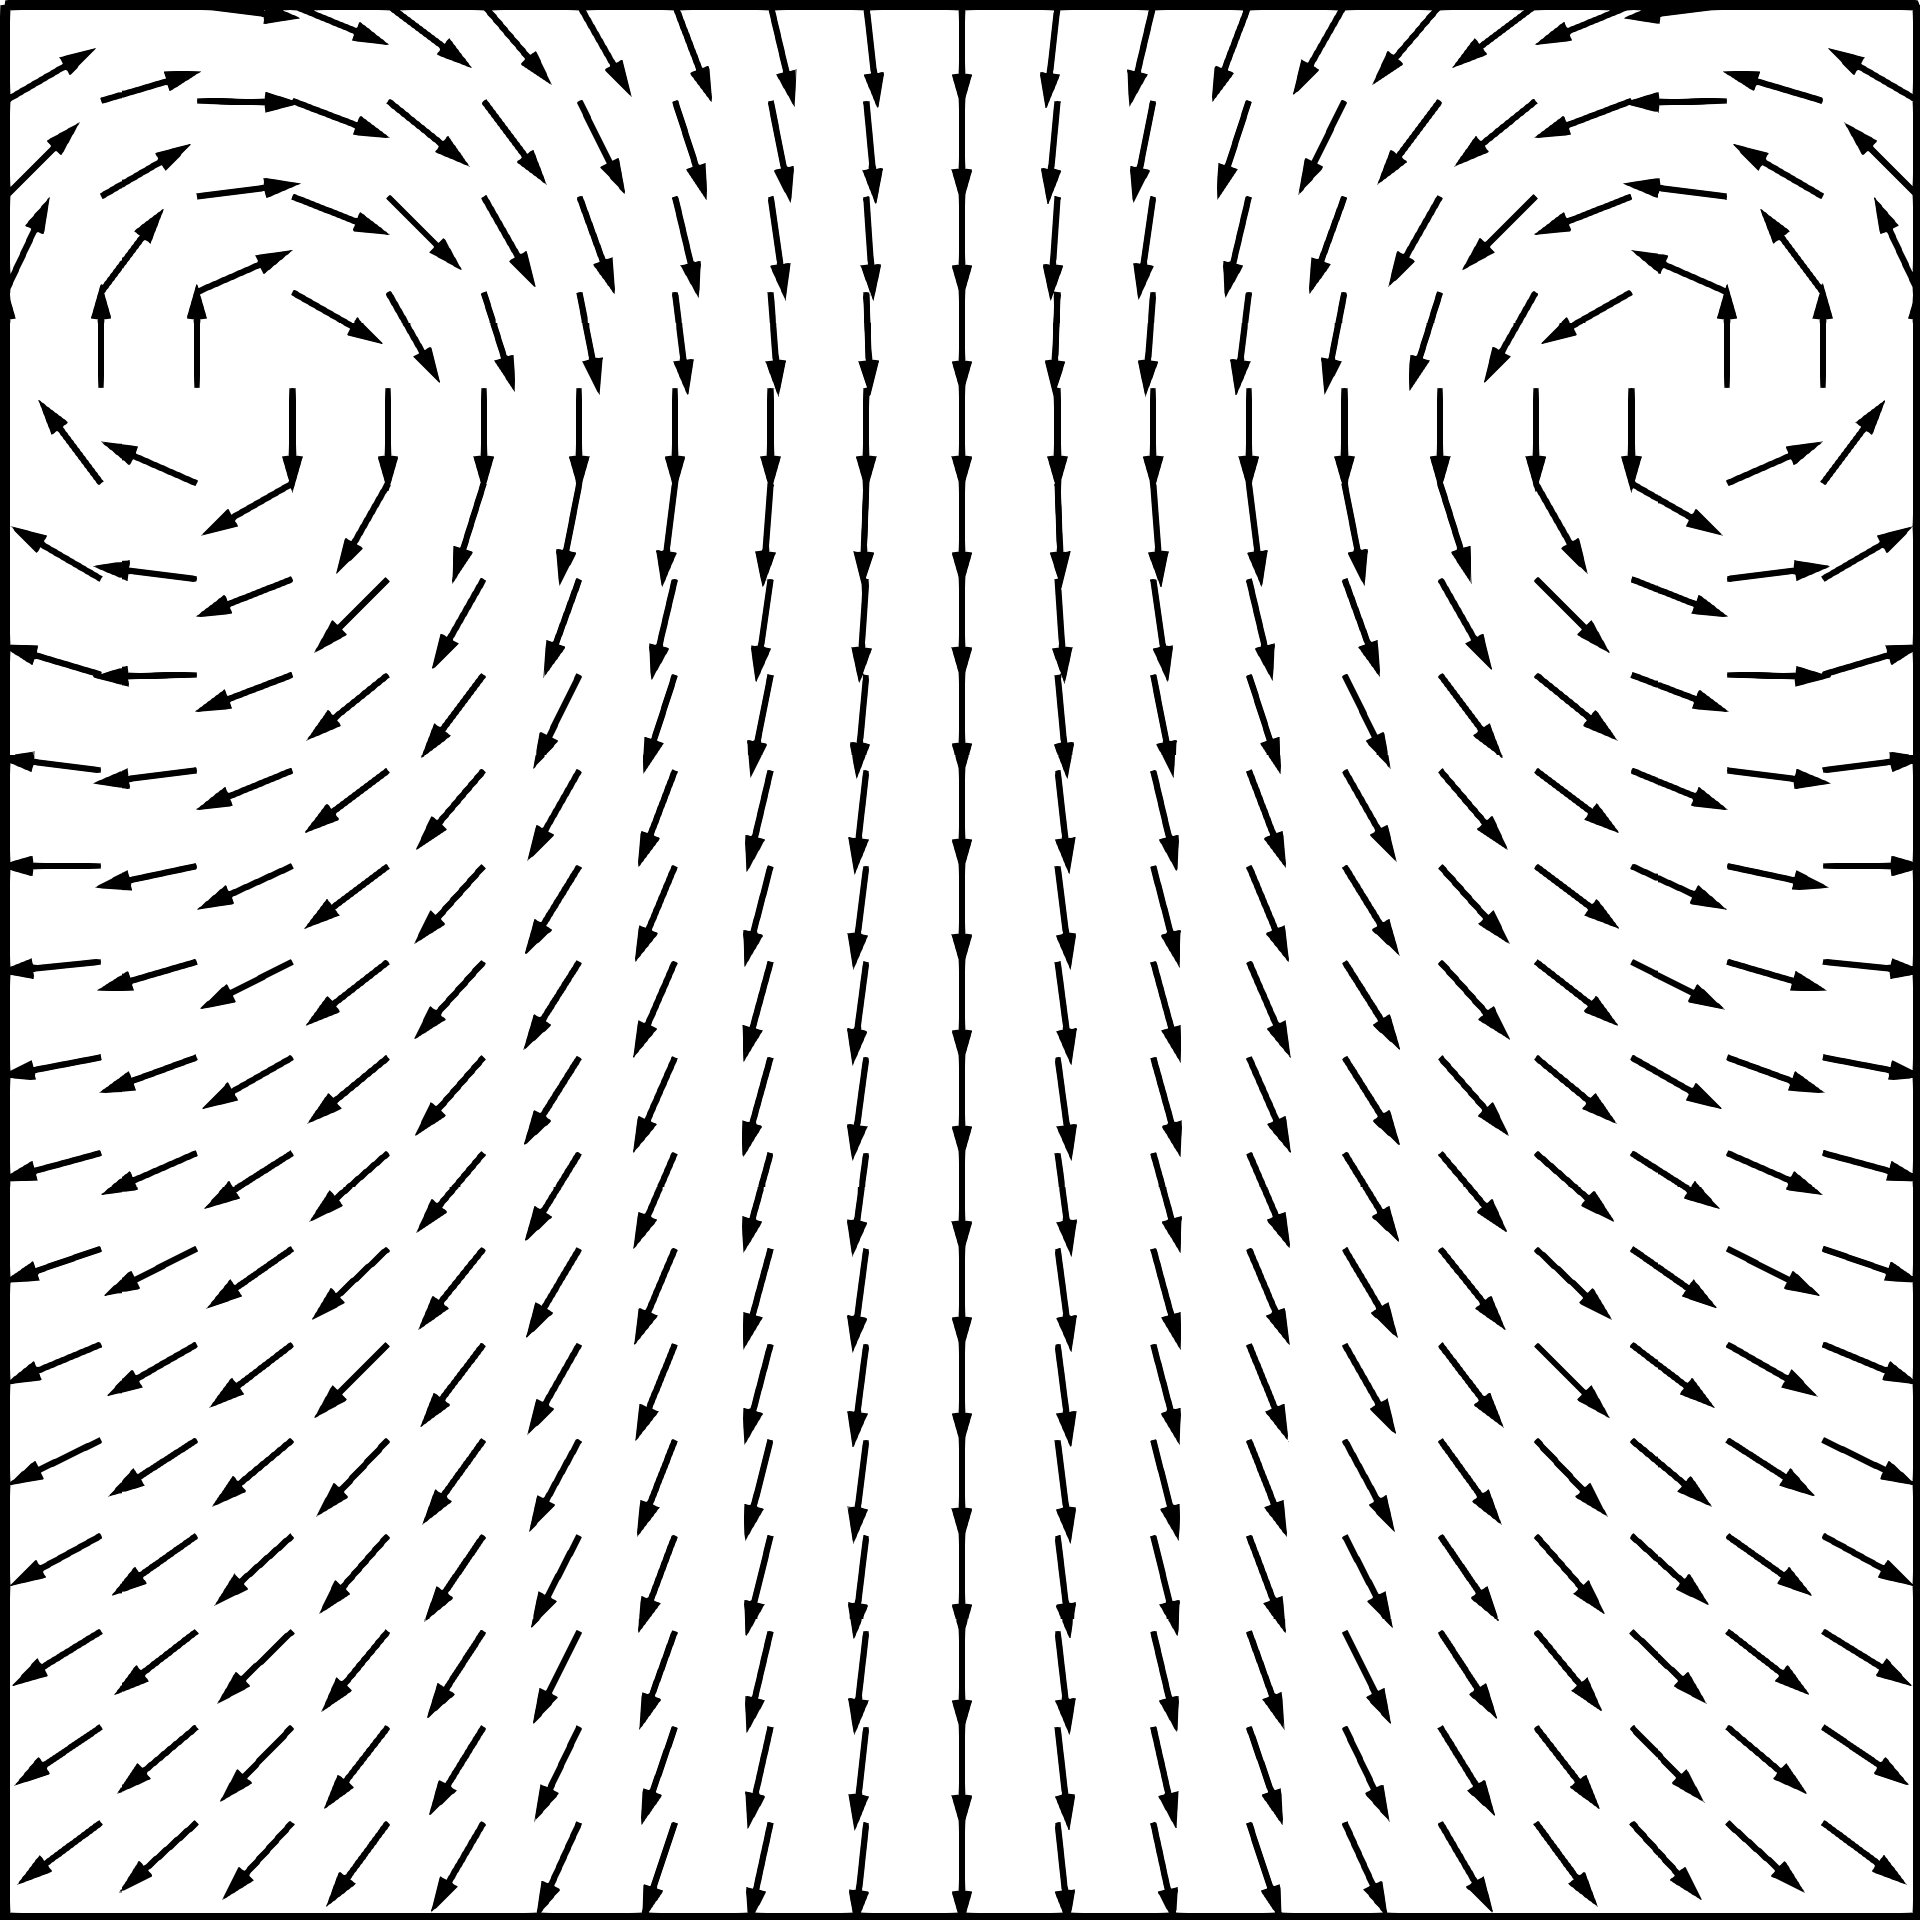
\includegraphics[scale=.065]{figures/Coaxing/Glyphs.png}
        \caption*{(a)}
    \end{subfigure}
    \begin{subfigure}{.24\textwidth}
        \centering
        
\includegraphics[scale=.065]{figures/Coaxing/SingleLine0.png}
        \caption*{(b)}
    \end{subfigure}
    \begin{subfigure}{.24\textwidth}
        \centering
        
\includegraphics[scale=.065]{figures/Coaxing/SingleLine1.png}
        \caption*{(c)}
    \end{subfigure}
    \begin{subfigure}{.24\textwidth}
        \centering
        
\includegraphics[scale=.065]{figures/Coaxing/SingleLine2.png}
        \caption*{(d)}
    \end{subfigure}
    \caption{
        Lines may diverge from the same origin when using $\alpha=0$. The field in this figure is $steady$.
        (a): We use the double gyre to show divergent behavior in (d), visualized with an arrow plot.
        (b): The initial seed and starting line length.
        (c): Random move and lengthen steps reach a local minimum energy by increasing streamline length, choosing a side at random.
        (d): A different result may occur with the same starting conditions.
    }
    \label[figure]{fig:energydevelopment}
\end{figure}
\noindent Since we compare many images and footprints from this subsection onward, it is useful to include a distinction using different color channels.
To save caption space, we use a consistent coloring to show streamline movement between time frames.
\textbf{Streamlines} are drawn in white, and we only draw them for the current time step.
\textbf{Footprints} from the current frame's streamlines are drawn in green, those from the last step in red.
The higher the intensity of a pixel, the stronger the energy in that region.
High time coherence therefore leads to most of the image being yellow, with few red or green areas.
We only draw the footprints obtained using the filter $L_t$, as those from $L_s$ can be easily inferred while
$L_t$ provides more visual clarity due to the reduced blur radius.
\begin{leftbar}
    \noindent \textbf{Note}: The algorithm may perform a combination of move and lengthen operations at once.
    Even with a constant field, it is possible for streamlines to move around or change their length slightly due to this inherent randomness.
    % Nonetheless, this section will give an accurate overview of how changing $\alpha$ impacts image quality.
\end{leftbar}

\noindent We now take a closer look at the energy development for different line positions seen in \cref{fig:energydevelopment} (a-d).
\noindent We start with a simple, steady field shown in (a), and a constant starting position for every execution at the center (b).
After 100 optimization steps, the streamline has grown to the maximum length possible (c), thereby reaching a minimum in spatial energy.
(d): The two likely outcomes of how the starting line develops under the specified starting conditions.
\begin{figure}[ht]
    \centering
    \begin{subfigure}{.22\textwidth}
        \centering
        
\includegraphics[scale=.06]{figures/Coaxing/SingleLine2.png}
        \caption*{(d)}
    \end{subfigure}
    \begin{subfigure}{.22\textwidth}
        \centering
        
\includegraphics[scale=.06]{figures/Coaxing/SingleLineC1.png}
        \caption*{(e)}
    \end{subfigure}
    \begin{subfigure}{.24\textwidth}
        \centering
        \resizebox{1.08\textwidth}{!}{
            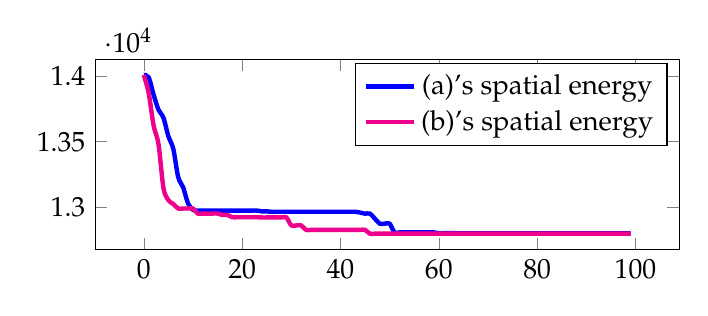
\begin{tikzpicture}
    \begin{axis} [
        width=9cm,
        height=4cm,
        every axis plot post/.append style={ultra thick, mark=none},
        xlabel=,
        ylabel=,
        x tick scale label style={},
    ]
        % Separate        
        \addplot +[smooth] [color=blue] coordinates {
            (0, 14007.826)
            (1, 13989.577)
            (2, 13856.987)
            (3, 13741.918)
            (4, 13681.778)
            (5, 13540.625)
            (6, 13445.154)
            (7, 13229.154)
            (8, 13151.793)
            (9, 13028.149)
            (10, 12979.961)
            (11, 12974.256)
            (12, 12974.256)
            (13, 12974.256)
            (14, 12974.256)
            (15, 12974.256)
            (16, 12974.256)
            (17, 12974.256)
            (18, 12974.256)
            (19, 12974.256)
            (20, 12974.256)
            (21, 12974.256)
            (22, 12974.256)
            (23, 12974.256)
            (24, 12968.2)
            (25, 12968.2)
            (26, 12965.026)
            (27, 12965.026)
            (28, 12965.026)
            (29, 12965.026)
            (30, 12965.026)
            (31, 12965.026)
            (32, 12965.026)
            (33, 12965.026)
            (34, 12965.026)
            (35, 12965.026)
            (36, 12965.026)
            (37, 12965.026)
            (38, 12965.026)
            (39, 12965.026)
            (40, 12965.026)
            (41, 12965.026)
            (42, 12965.026)
            (43, 12965.026)
            (44, 12959.116)
            (45, 12950.877)
            (46, 12950.877)
            (47, 12912.311)
            (48, 12874.413)
            (49, 12874.413)
            (50, 12874.413)
            (51, 12807.514)
            (52, 12807.514)
            (53, 12807.514)
            (54, 12807.514)
            (55, 12807.514)
            (56, 12807.514)
            (57, 12807.514)
            (58, 12807.514)
            (59, 12807.514)
            (60, 12801.792)
            (61, 12801.792)
            (62, 12801.792)
            (63, 12801.792)
            (64, 12801.289)
            (65, 12801.289)
            (66, 12801.289)
            (67, 12801.289)
            (68, 12801.289)
            (69, 12801.289)
            (70, 12801.289)
            (71, 12801.289)
            (72, 12801.289)
            (73, 12801.289)
            (74, 12801.289)
            (75, 12801.289)
            (76, 12801.289)
            (77, 12801.289)
            (78, 12801.289)
            (79, 12801.289)
            (80, 12801.289)
            (81, 12801.289)
            (82, 12801.289)
            (83, 12801.289)
            (84, 12801.289)
            (85, 12801.289)
            (86, 12801.289)
            (87, 12801.289)
            (88, 12801.289)
            (89, 12801.289)
            (90, 12801.289)
            (91, 12801.289)
            (92, 12801.289)
            (93, 12801.289)
            (94, 12801.289)
            (95, 12801.289)
            (96, 12801.289)
            (97, 12801.289)
            (98, 12801.289)
            (99, 12801.289)
        };
        % Overlapping
        \addplot +[smooth] [color=magenta] coordinates {
            (0, 14007.826) 
            (1, 13869.016) 
            (2, 13622.305) 
            (3, 13479.086) 
            (4, 13146.85)  
            (5, 13052.909) 
            (6, 13024.708) 
            (7, 12989.768) 
            (8, 12989.768) 
            (9, 12989.768) 
            (10, 12989.768)
            (11, 12951.466)
            (12, 12951.466)
            (13, 12951.466)
            (14, 12951.466)
            (15, 12951.466)
            (16, 12940.784)
            (17, 12940.784)
            (18, 12923.523)
            (19, 12923.523)
            (20, 12923.523)
            (21, 12923.523)
            (22, 12923.523)
            (23, 12923.523)
            (24, 12921.698)
            (25, 12921.698)
            (26, 12921.698)
            (27, 12921.698)
            (28, 12921.698)
            (29, 12921.698)
            (30, 12860.99) 
            (31, 12860.99) 
            (32, 12860.99)
            (33, 12827.076)
            (34, 12827.076)
            (35, 12827.076)
            (36, 12827.076)
            (37, 12827.076)
            (38, 12827.076)
            (39, 12827.076)
            (40, 12827.076)
            (41, 12827.076)
            (42, 12827.076)
            (43, 12827.076)
            (44, 12827.076)
            (45, 12827.076)
            (46, 12798.14)
            (47, 12798.14)
            (48, 12798.14)
            (49, 12798.14)
            (50, 12798.14)
            (51, 12798.14)
            (52, 12798.14)
            (53, 12798.14)
            (54, 12798.14)
            (55, 12798.14)
            (56, 12798.14)
            (57, 12798.14)
            (58, 12798.14)
            (59, 12798.14)
            (60, 12798.14)
            (61, 12798.14)
            (62, 12798.14)
            (63, 12798.14)
            (64, 12798.14)
            (65, 12798.14)
            (66, 12798.14)
            (67, 12798.14)
            (68, 12798.14)
            (69, 12798.14)
            (70, 12798.14)
            (71, 12798.14)
            (72, 12798.14)
            (73, 12798.14)
            (74, 12798.14)
            (75, 12798.14)
            (76, 12798.14)
            (77, 12798.14)
            (78, 12798.14)
            (79, 12798.14)
            (80, 12798.14)
            (81, 12798.14)
            (82, 12798.14)
            (83, 12798.14)
            (84, 12798.14)
            (85, 12798.14)
            (86, 12798.14)
            (87, 12798.14)
            (88, 12798.14)
            (89, 12798.14)
            (90, 12798.14)
            (91, 12798.14)
            (92, 12798.14)
            (93, 12798.14)
            (94, 12798.14)
            (95, 12798.14)
            (96, 12798.14)
            (97, 12798.14)
            (98, 12798.14)
            (99, 12798.14)
        };
        \addlegendentry{(a)'s spatial energy}
        \addlegendentry{(b)'s spatial energy}
    \end{axis}
\end{tikzpicture}

        }
        \caption*{(f)}
    \end{subfigure}
    \begin{subfigure}{.24\textwidth}
        \centering
        \resizebox{1.08\textwidth}{!}{
            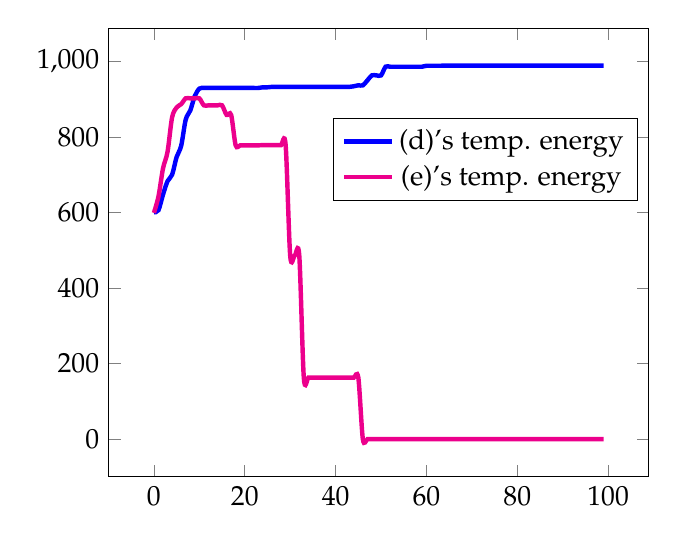
\begin{tikzpicture}
    \begin{axis} [
        every axis plot post/.append style={ultra thick, mark=none}, 
        xlabel=,
        legend style={at={(.98,.8)},anchor=north east}
    ]
        \addplot +[smooth] [color=blue] coordinates {
            (0, 600.738)
            (1, 606.401)
            (2, 647.542)
            (3, 683.247)
            (4, 700.14)
            (5, 747.113)
            (6, 776.618)
            (7, 846.143)
            (8, 870.048)
            (9, 908.393)
            (10, 928.066)
            (11, 929.862)
            (12, 929.862)
            (13, 929.862)
            (14, 929.862)
            (15, 929.862)
            (16, 929.862)
            (17, 929.862)
            (18, 929.862)
            (19, 929.862)
            (20, 929.862)
            (21, 929.862)
            (22, 929.862)
            (23, 929.862)
            (24, 931.591)
            (25, 931.591)
            (26, 932.786)
            (27, 932.786)
            (28, 932.786)
            (29, 932.786)
            (30, 932.786)
            (31, 932.786)
            (32, 932.786)
            (33, 932.786)
            (34, 932.786)
            (35, 932.786)
            (36, 932.786)
            (37, 932.786)
            (38, 932.786)
            (39, 932.786)
            (40, 932.786)
            (41, 932.786)
            (42, 932.786)
            (43, 932.786)
            (44, 934.333)
            (45, 936.797)
            (46, 936.797)
            (47, 949.954)
            (48, 963.133)
            (49, 963.133)
            (50, 963.133)
            (51, 986.039)
            (52, 986.039)
            (53, 986.039)
            (54, 986.039)
            (55, 986.039)
            (56, 986.039)
            (57, 986.039)
            (58, 986.039)
            (59, 986.039)
            (60, 988.596)
            (61, 988.596)
            (62, 988.596)
            (63, 988.596)
            (64, 989.078)
            (65, 989.078)
            (66, 989.078)
            (67, 989.078)
            (68, 989.078)
            (69, 989.078)
            (70, 989.078)
            (71, 989.078)
            (72, 989.078)
            (73, 989.078)
            (74, 989.078)
            (75, 989.078)
            (76, 989.078)
            (77, 989.078)
            (78, 989.078)
            (79, 989.078)
            (80, 989.078)
            (81, 989.078)
            (82, 989.078)
            (83, 989.078)
            (84, 989.078)
            (85, 989.078)
            (86, 989.078)
            (87, 989.078)
            (88, 989.078)
            (89, 989.078)
            (90, 989.078)
            (91, 989.078)
            (92, 989.078)
            (93, 989.078)
            (94, 989.078)
            (95, 989.078)
            (96, 989.078)
            (97, 989.078)
            (98, 989.078)
            (99, 989.078)    
        };
        \addplot +[smooth] [color=magenta] coordinates {
            (0, 599.266) 
            (1, 642.339) 
            (2, 716.691) 
            (3, 760.73)  
            (4, 851.884) 
            (5, 878.242) 
            (6, 886.961) 
            (7, 902.354) 
            (8, 902.354) 
            (9, 902.354) 
            (10, 902.354)
            (11, 883.831)
            (12, 883.831)
            (13, 883.831)
            (14, 883.831)
            (15, 883.831)
            (16, 858.702)
            (17, 858.702)
            (18, 777.924)
            (19, 777.924)
            (20, 777.924)
            (21, 777.924)
            (22, 777.924)
            (23, 777.924)
            (24, 778.653)
            (25, 778.653)
            (26, 778.653)
            (27, 778.653)
            (28, 778.653)
            (29, 778.653)
            (30, 486.235)
            (31, 486.235)
            (32, 486.235)
            (33, 163.149)
            (34, 163.149)
            (35, 163.149)
            (36, 163.149)
            (37, 163.149)
            (38, 163.149)
            (39, 163.149)
            (40, 163.149)
            (41, 163.149)
            (42, 163.149)
            (43, 163.149)
            (44, 163.149)
            (45, 163.149)
            (46, 0.216)
            (47, 0.216)
            (48, 0.216)
            (49, 0.216)
            (50, 0.216)
            (51, 0.216)
            (52, 0.216)
            (53, 0.216)
            (54, 0.216)
            (55, 0.216)
            (56, 0.216)
            (57, 0.216)
            (58, 0.216)
            (59, 0.216)
            (60, 0.216)
            (61, 0.216)
            (62, 0.216)
            (63, 0.216)
            (64, 0.216)
            (65, 0.216)
            (66, 0.216)
            (67, 0.216)
            (68, 0.216)
            (69, 0.216)
            (70, 0.216)
            (71, 0.216)
            (72, 0.216)
            (73, 0.216)
            (74, 0.216)
            (75, 0.216)
            (76, 0.216)
            (77, 0.216)
            (78, 0.216)
            (79, 0.216)
            (80, 0.216)
            (81, 0.216)
            (82, 0.216)
            (83, 0.216)
            (84, 0.216)
            (85, 0.216)
            (86, 0.216)
            (87, 0.216)
            (88, 0.216)
            (89, 0.216)
            (90, 0.216)
            (91, 0.216)
            (92, 0.216)
            (93, 0.216)
            (94, 0.216)
            (95, 0.216)
            (96, 0.216)
            (97, 0.216)
            (98, 0.216)
            (99, 0.216)   
        };
        \addlegendentry{(d)'s temp. energy}
        \addlegendentry{(e)'s temp. energy}
    \end{axis}
\end{tikzpicture}

        }
        \caption*{(g)}
    \end{subfigure}
    \caption{
        (d): A different result may occur with the same starting conditions, the lengths are invariant in this case.
        (e): An example for an outcome in favor of temporal energy.
        (f): Spacial energy vs optimization steps.
        (g): Temporal energy vs optimization steps.
    }
\label[figure]{fig:energydevelopment2}
\end{figure}

We can see that due to the randomness of the algorithm, there is a $\approx50\%$ chance of ending up on either side of the center ridge (d).
\newpage
On \cref{fig:energydevelopment2} (f), we see a plot of the spatial energy vs the current optimization step. The maximum spatial energy equals the image resolution at 120x120.
Initially, we can see a stark decline in energy for both curves.
This is caused by to a fast lengthening process, with an average of about 2.5\% image size per step, per side.
The first plateau phase is reached after $\approx$ 15 steps, as the streamlines reach the edge of the domain and cannot lengthen further.
Due to the random movements, the line ends drift along the upper and lower domain borders, slowly lengthening due to the curvature.
A final stronger decline happens at 30 steps for (d), and at 50 steps for (e), as the curvature is strong enough do allow larger regions of spaces
to be filled by lengthening once again.
The delay between (d) and (e) is caused by the random nature of the algorithm, and is equal if both runs use the same seed.
Our streamline reaches the minimum possible energy of about 12500, with a difference of 1300.
Since the line length lies at roughly 140px and the filter is about 14px wide (note: $L_t$ as shown is half the size of $L_s$),
these numbers aren't surprising.

The temporal energy is shown on plot (g), where we can see a stark difference in the development of (d) and (e).
Many features regarding local rate of change are recognizable in both plots, e.g. the plateau of (e) centered around the 40th step's mark.
The final temporal difference lies at 1000 vs the spatial difference at 1300, again a result of the reduced filter radius.
\newpage

\begin{figure}[ht]
    \centering
    % 5 x No coherence
    \begin{subfigure}{\textwidth}
        \begin{subfigure}{.19\textwidth}
            \centering
            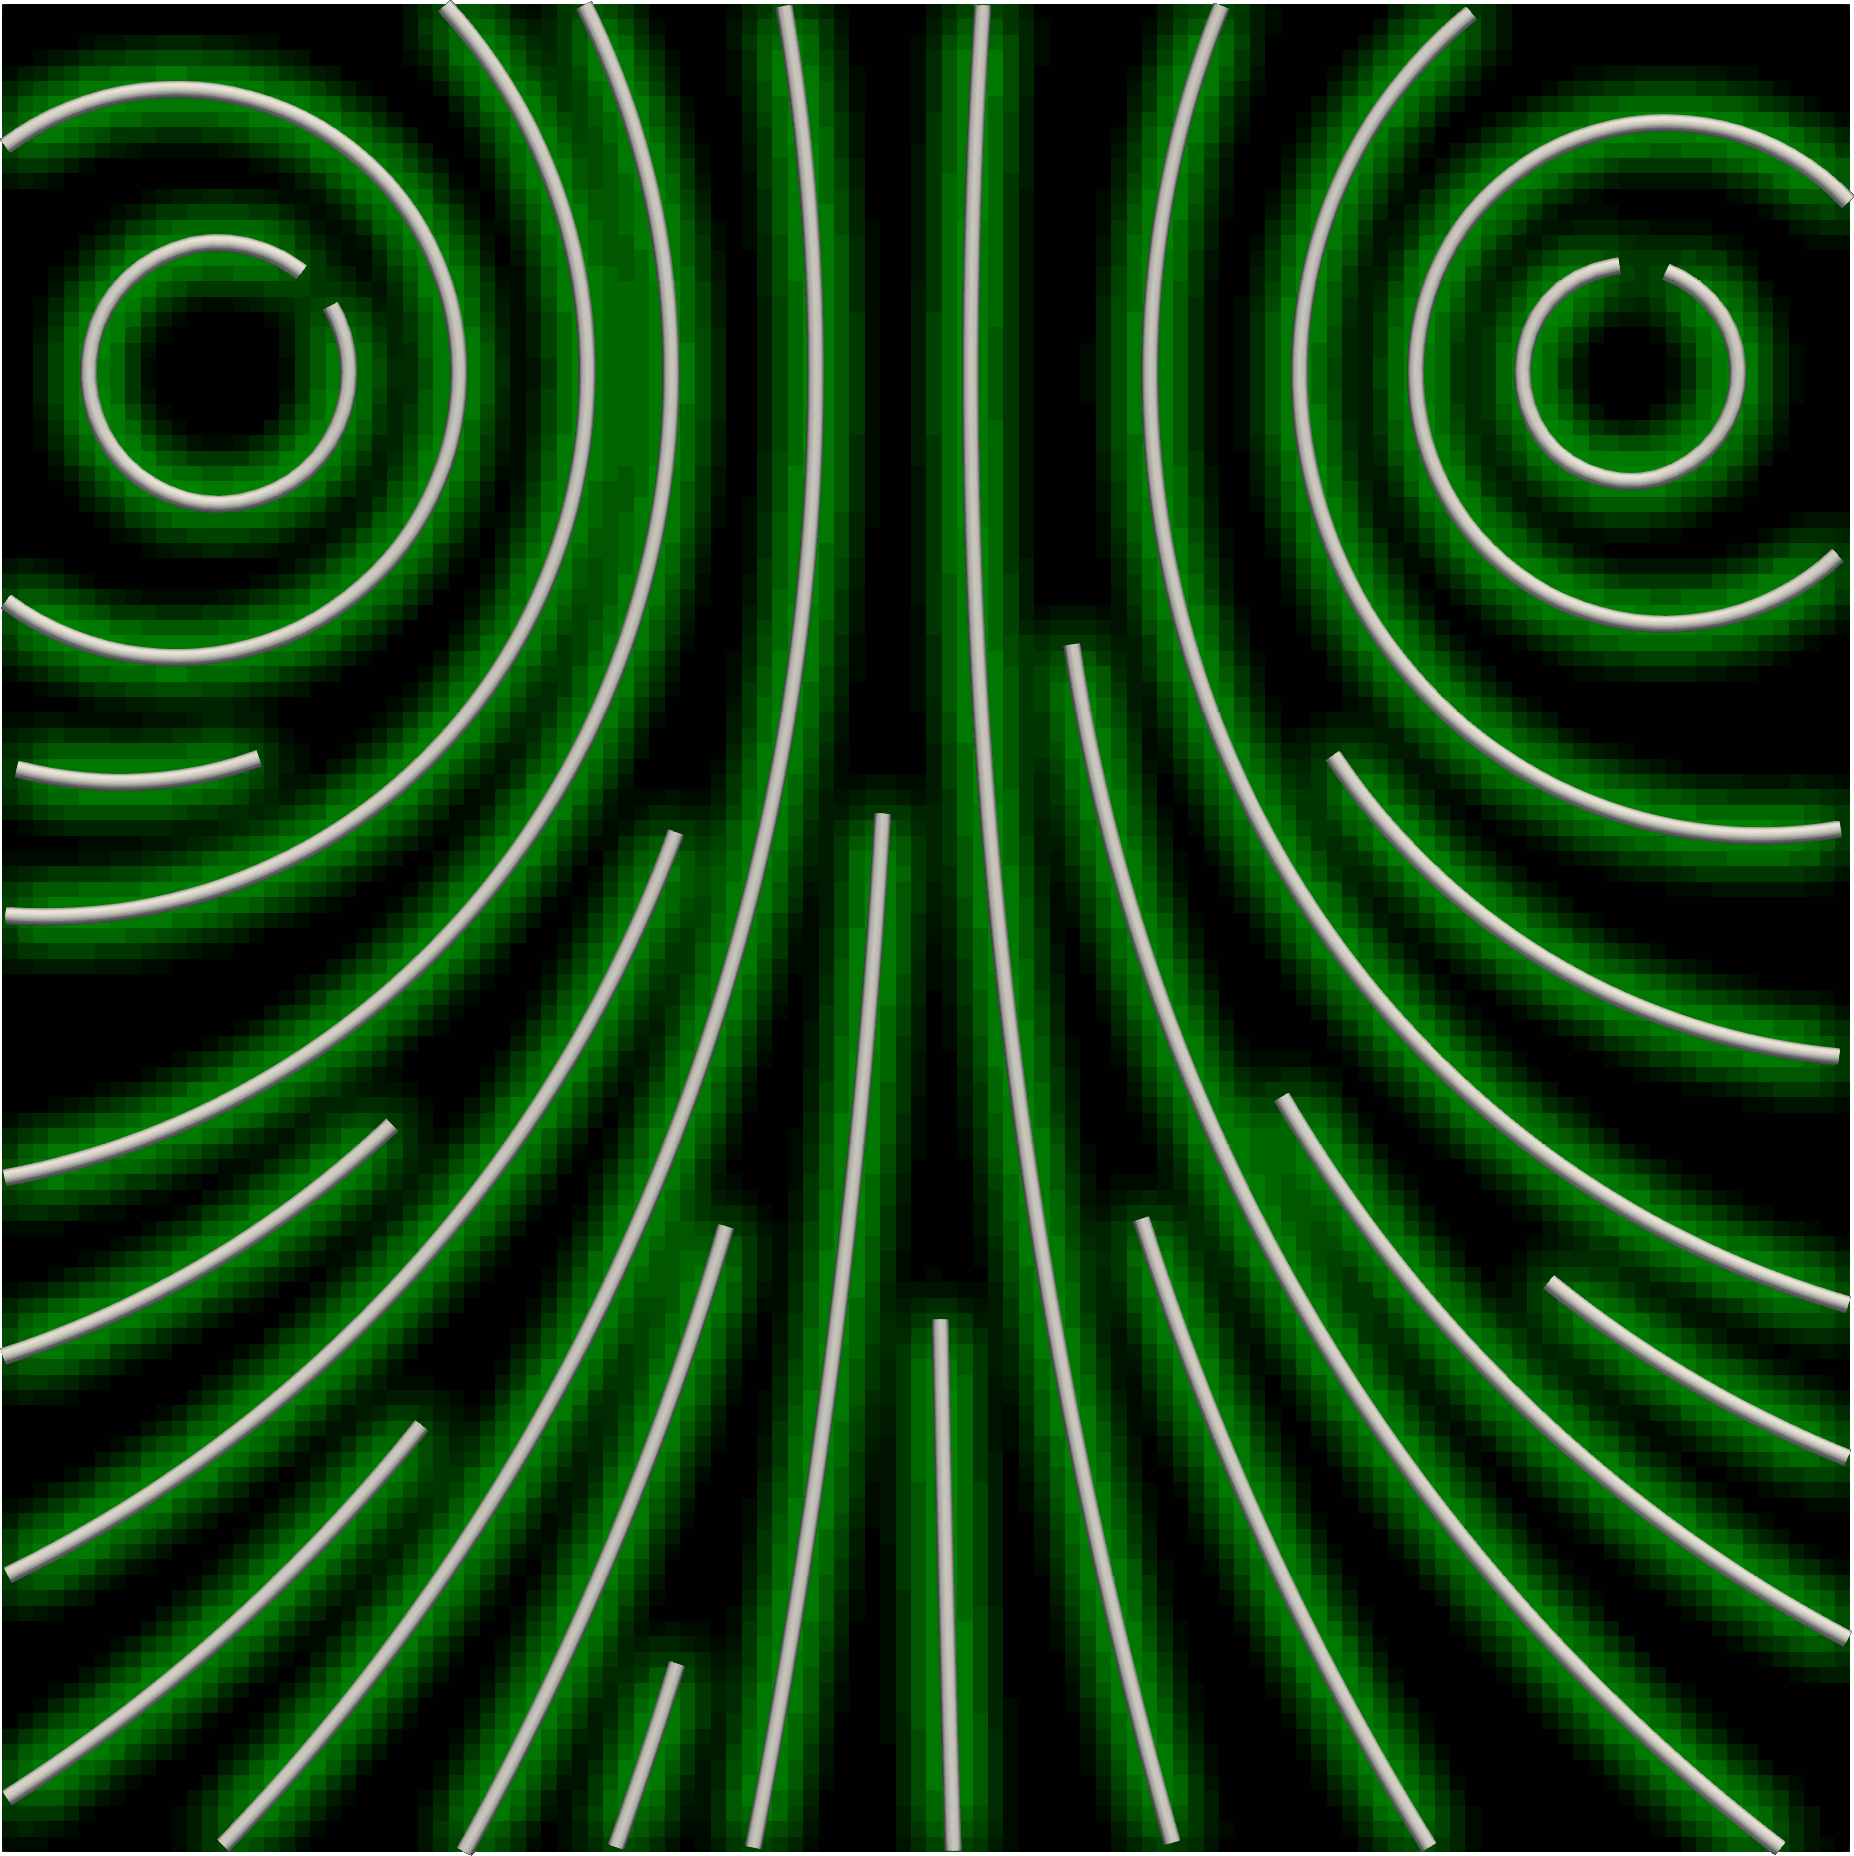
\includegraphics[scale=.055]{figures/AlphaStudy/GyroNC.0000.png}
        \end{subfigure}
        \begin{subfigure}{.19\textwidth}
            \centering
            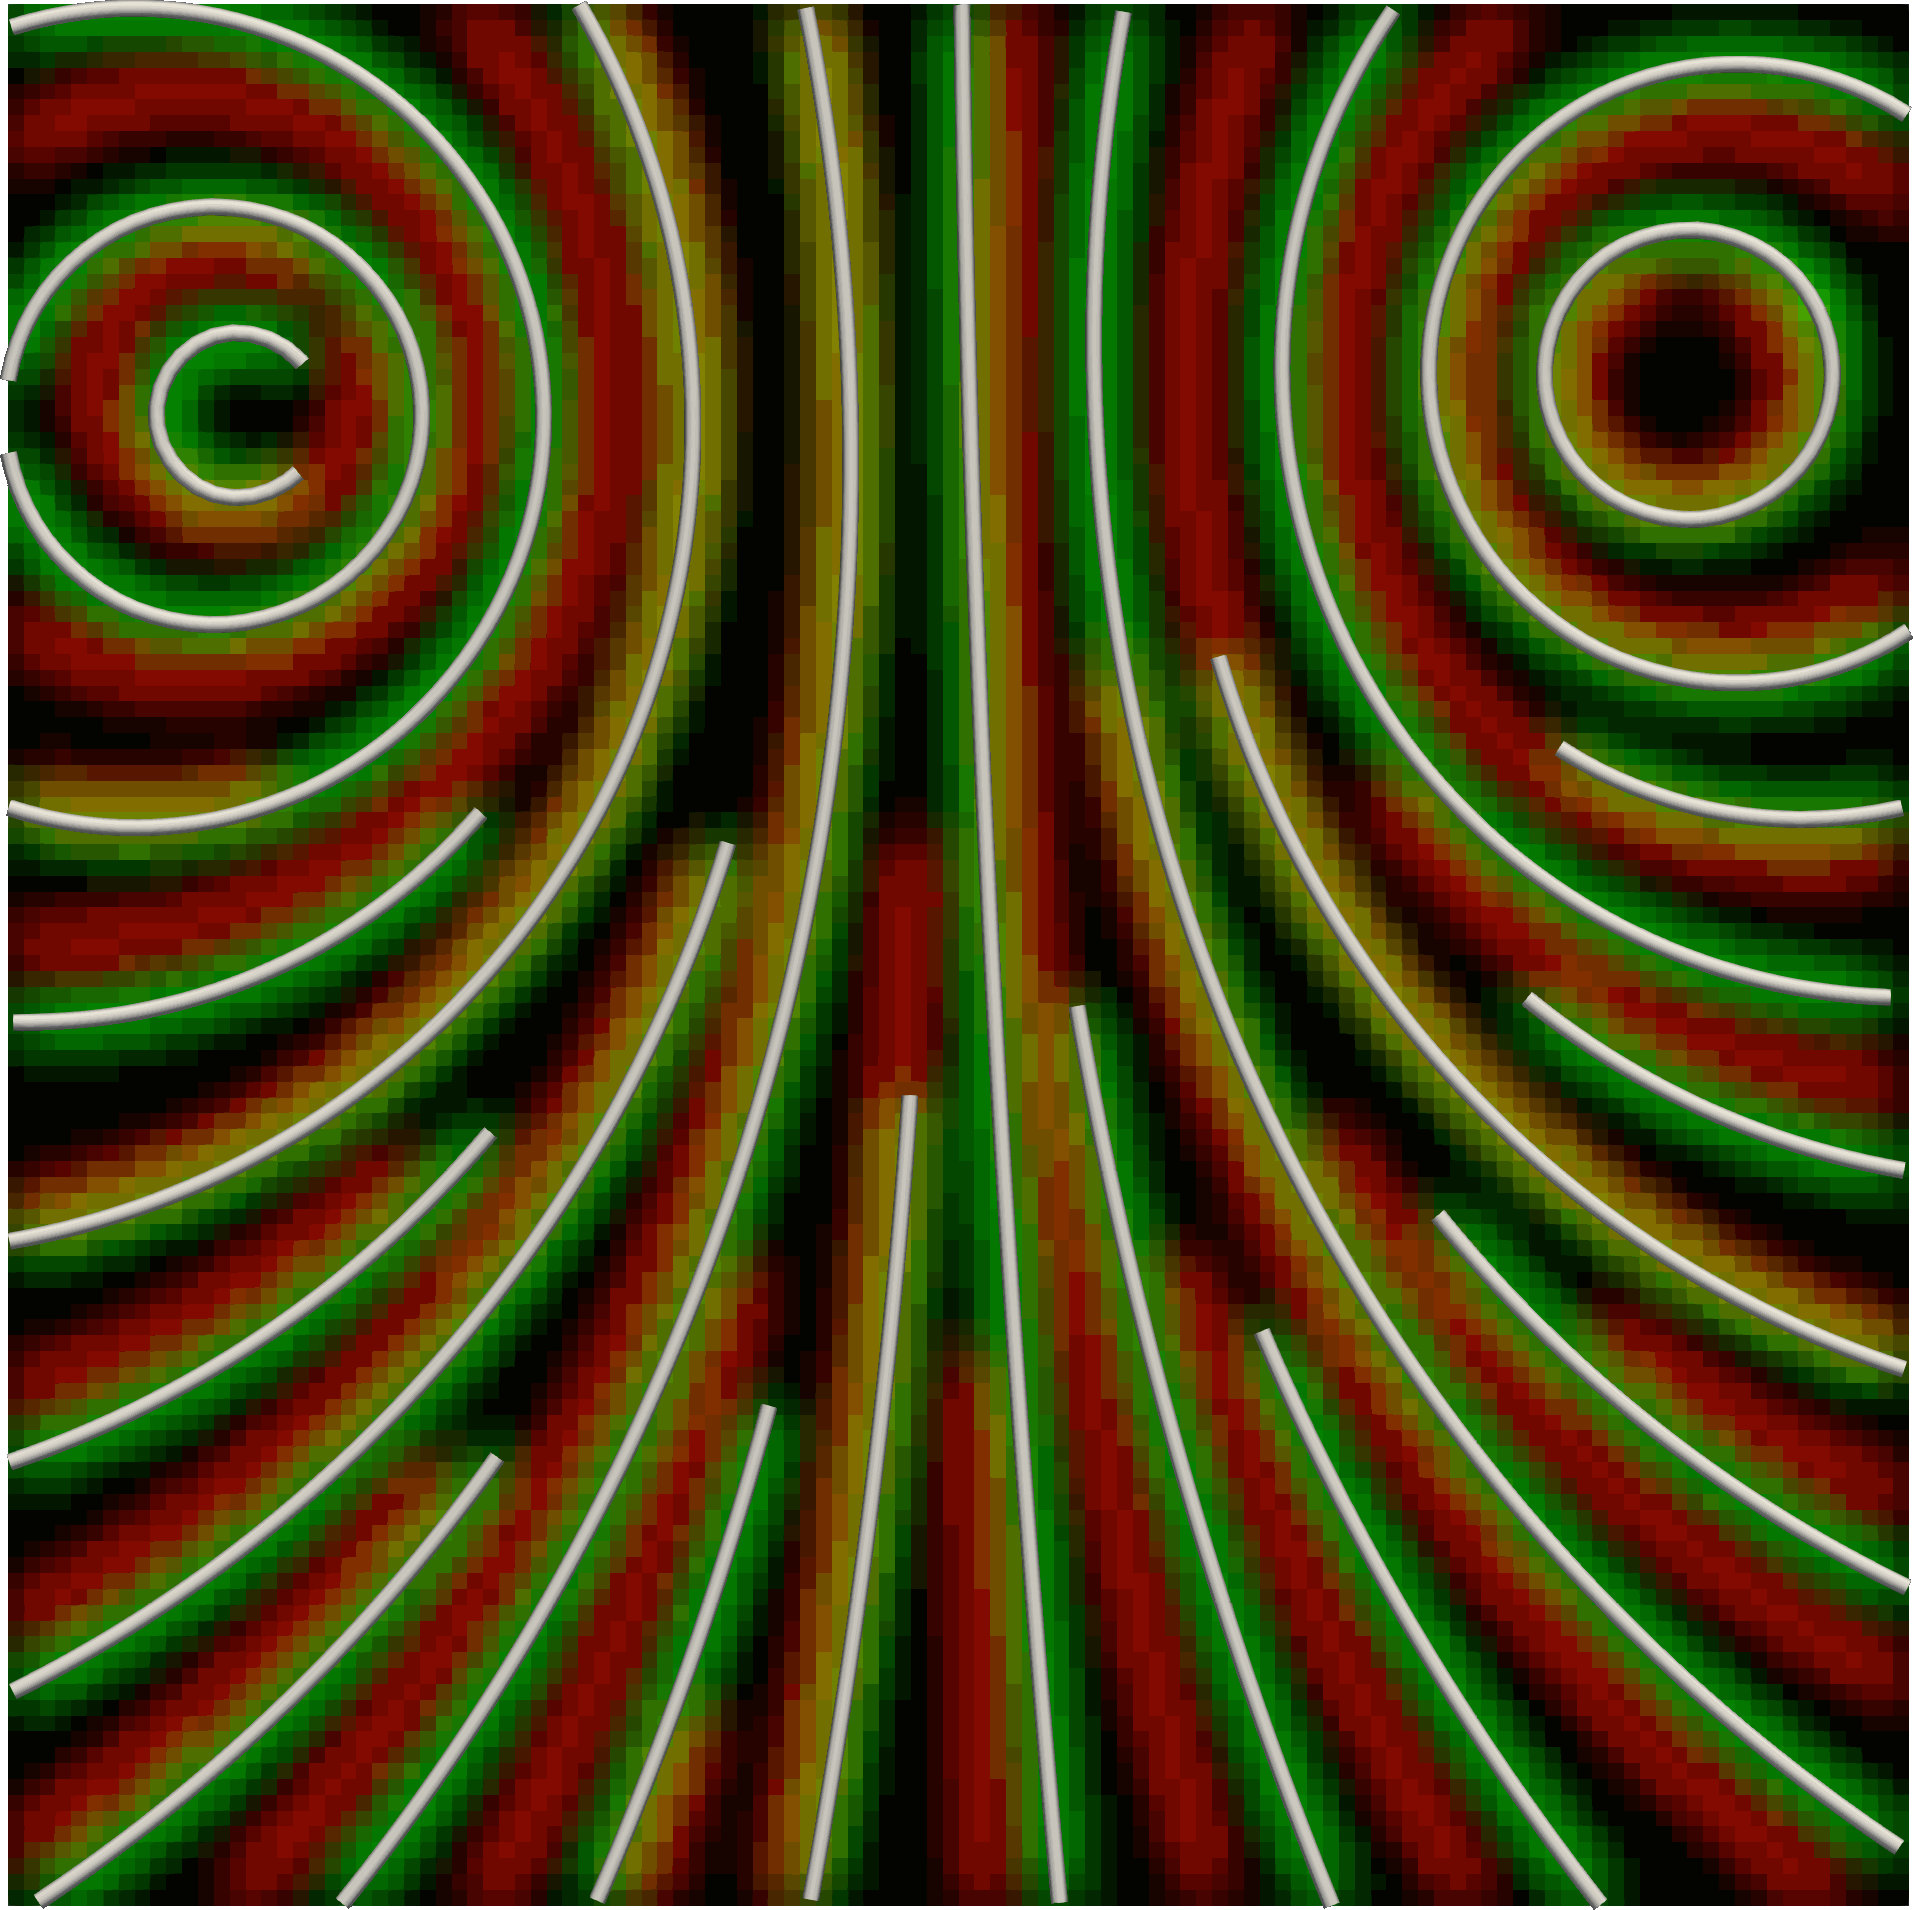
\includegraphics[scale=.0535]{figures/AlphaStudy/GyroNC.0001.png}
        \end{subfigure}
        \begin{subfigure}{.19\textwidth}
            \centering
            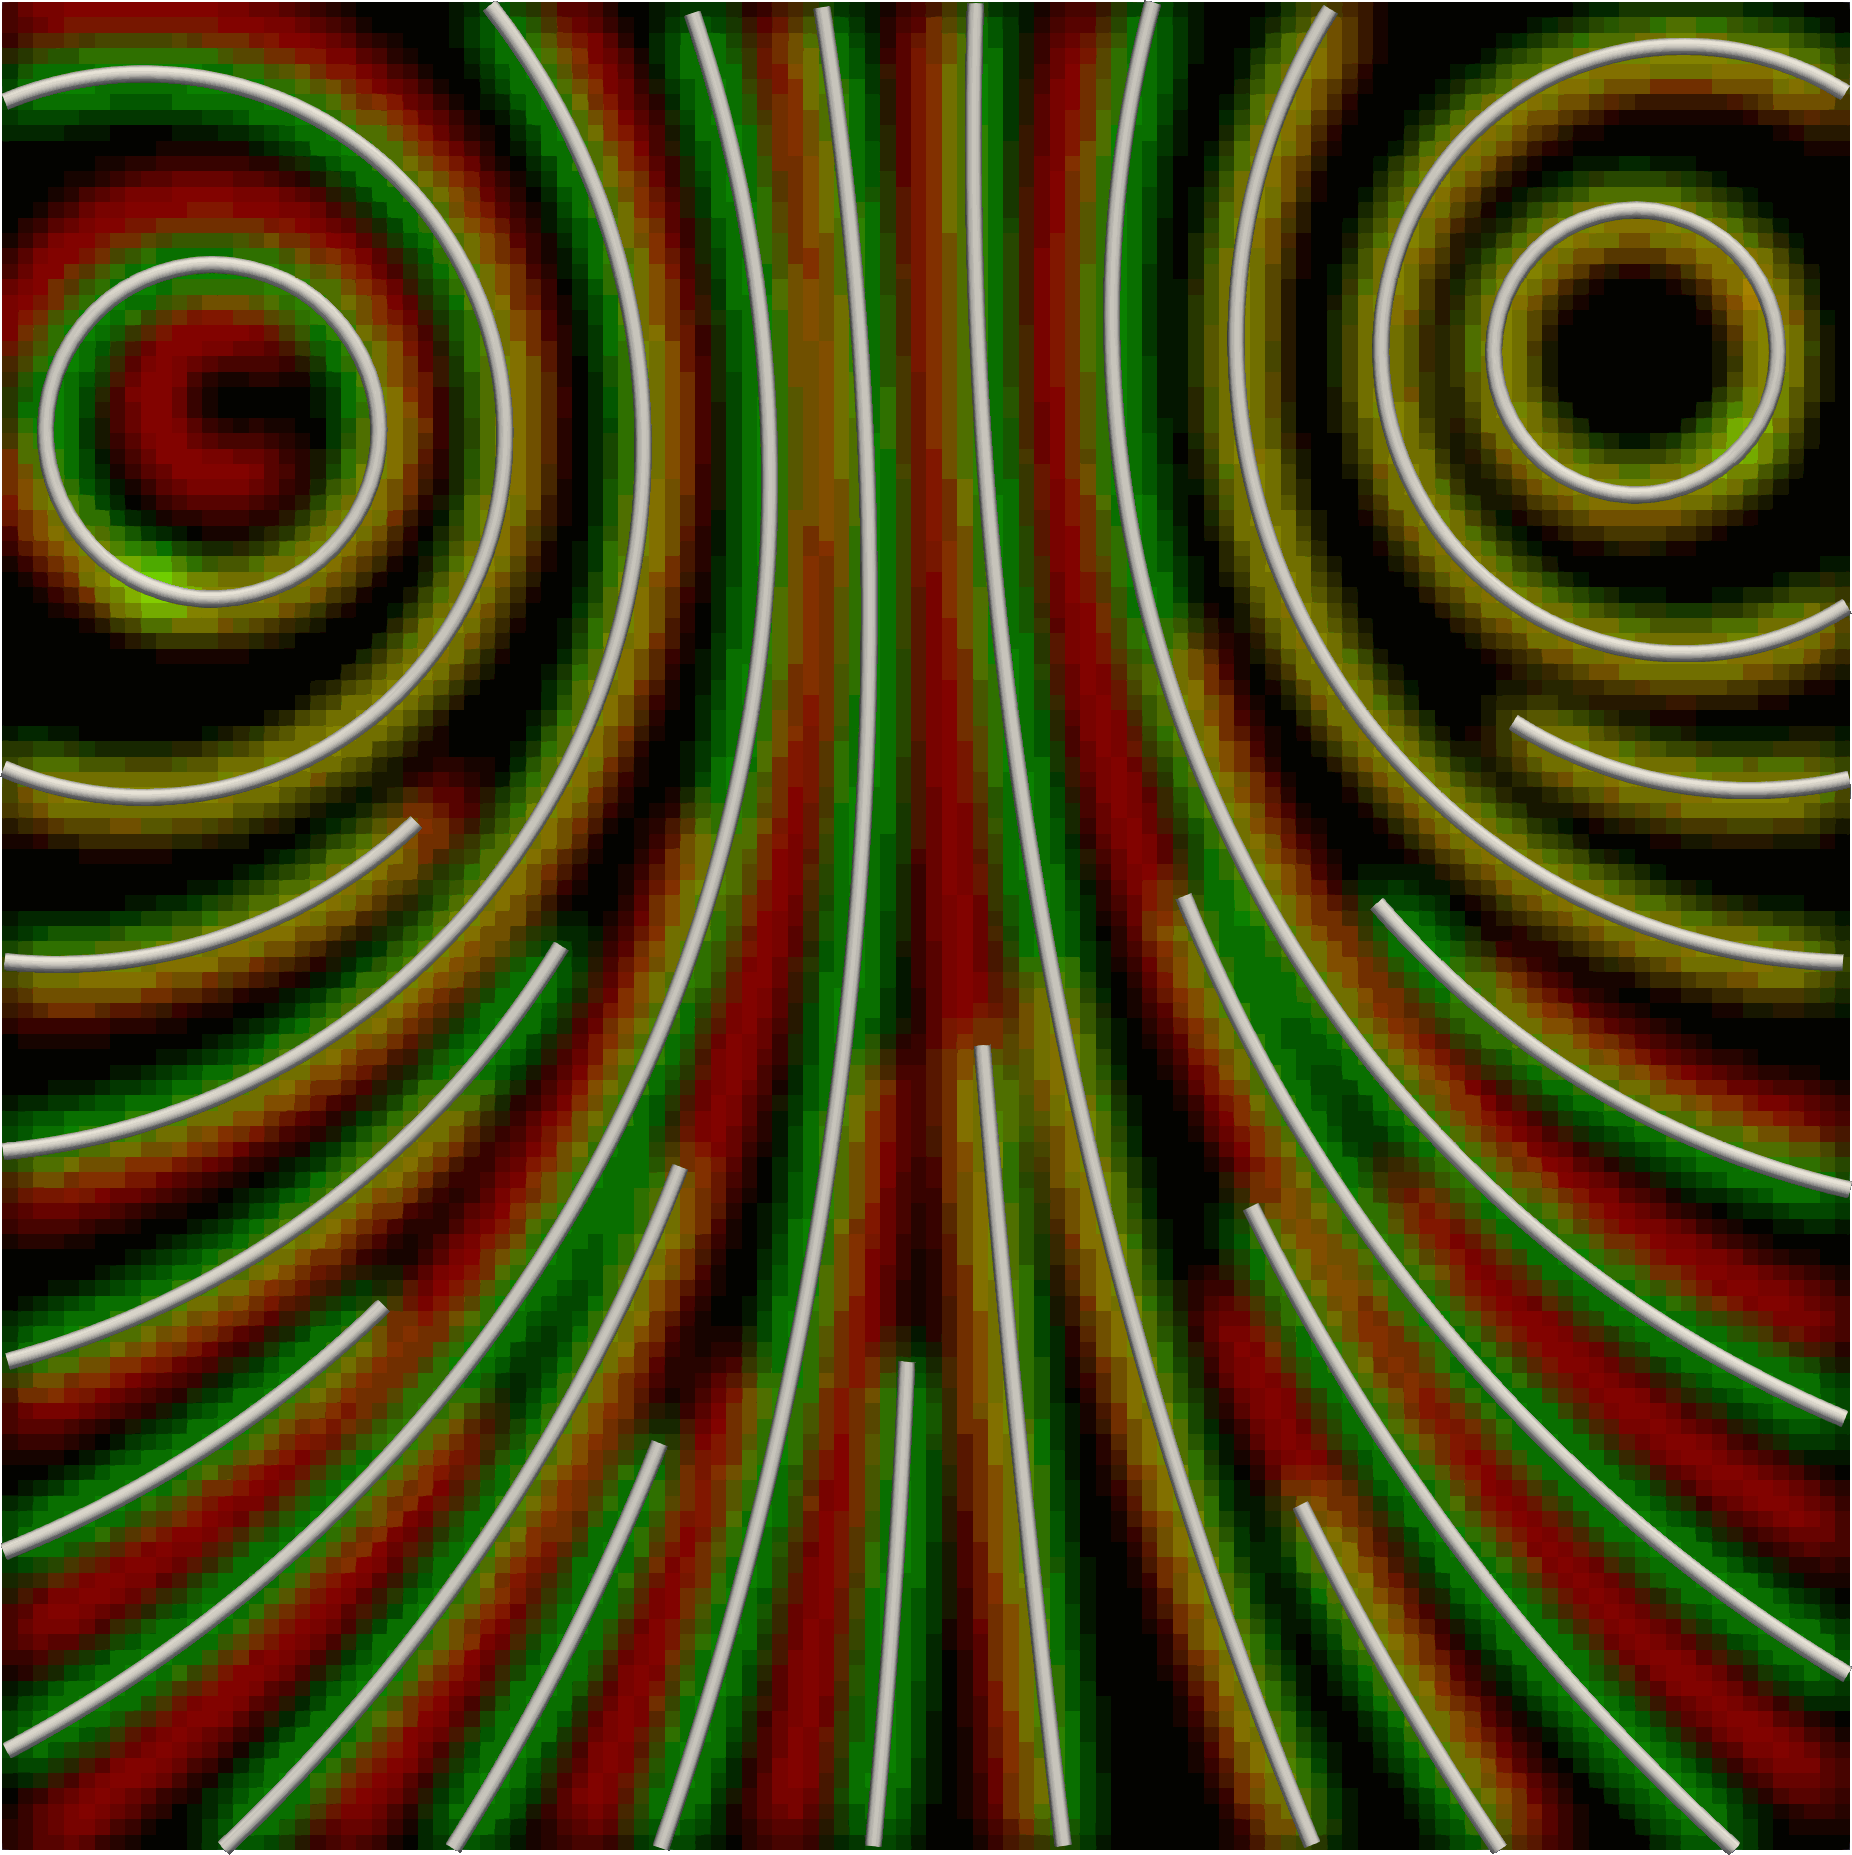
\includegraphics[scale=.055]{figures/AlphaStudy/GyroNC.0002.png}
        \end{subfigure}
        \begin{subfigure}{.19\textwidth}
            \centering
            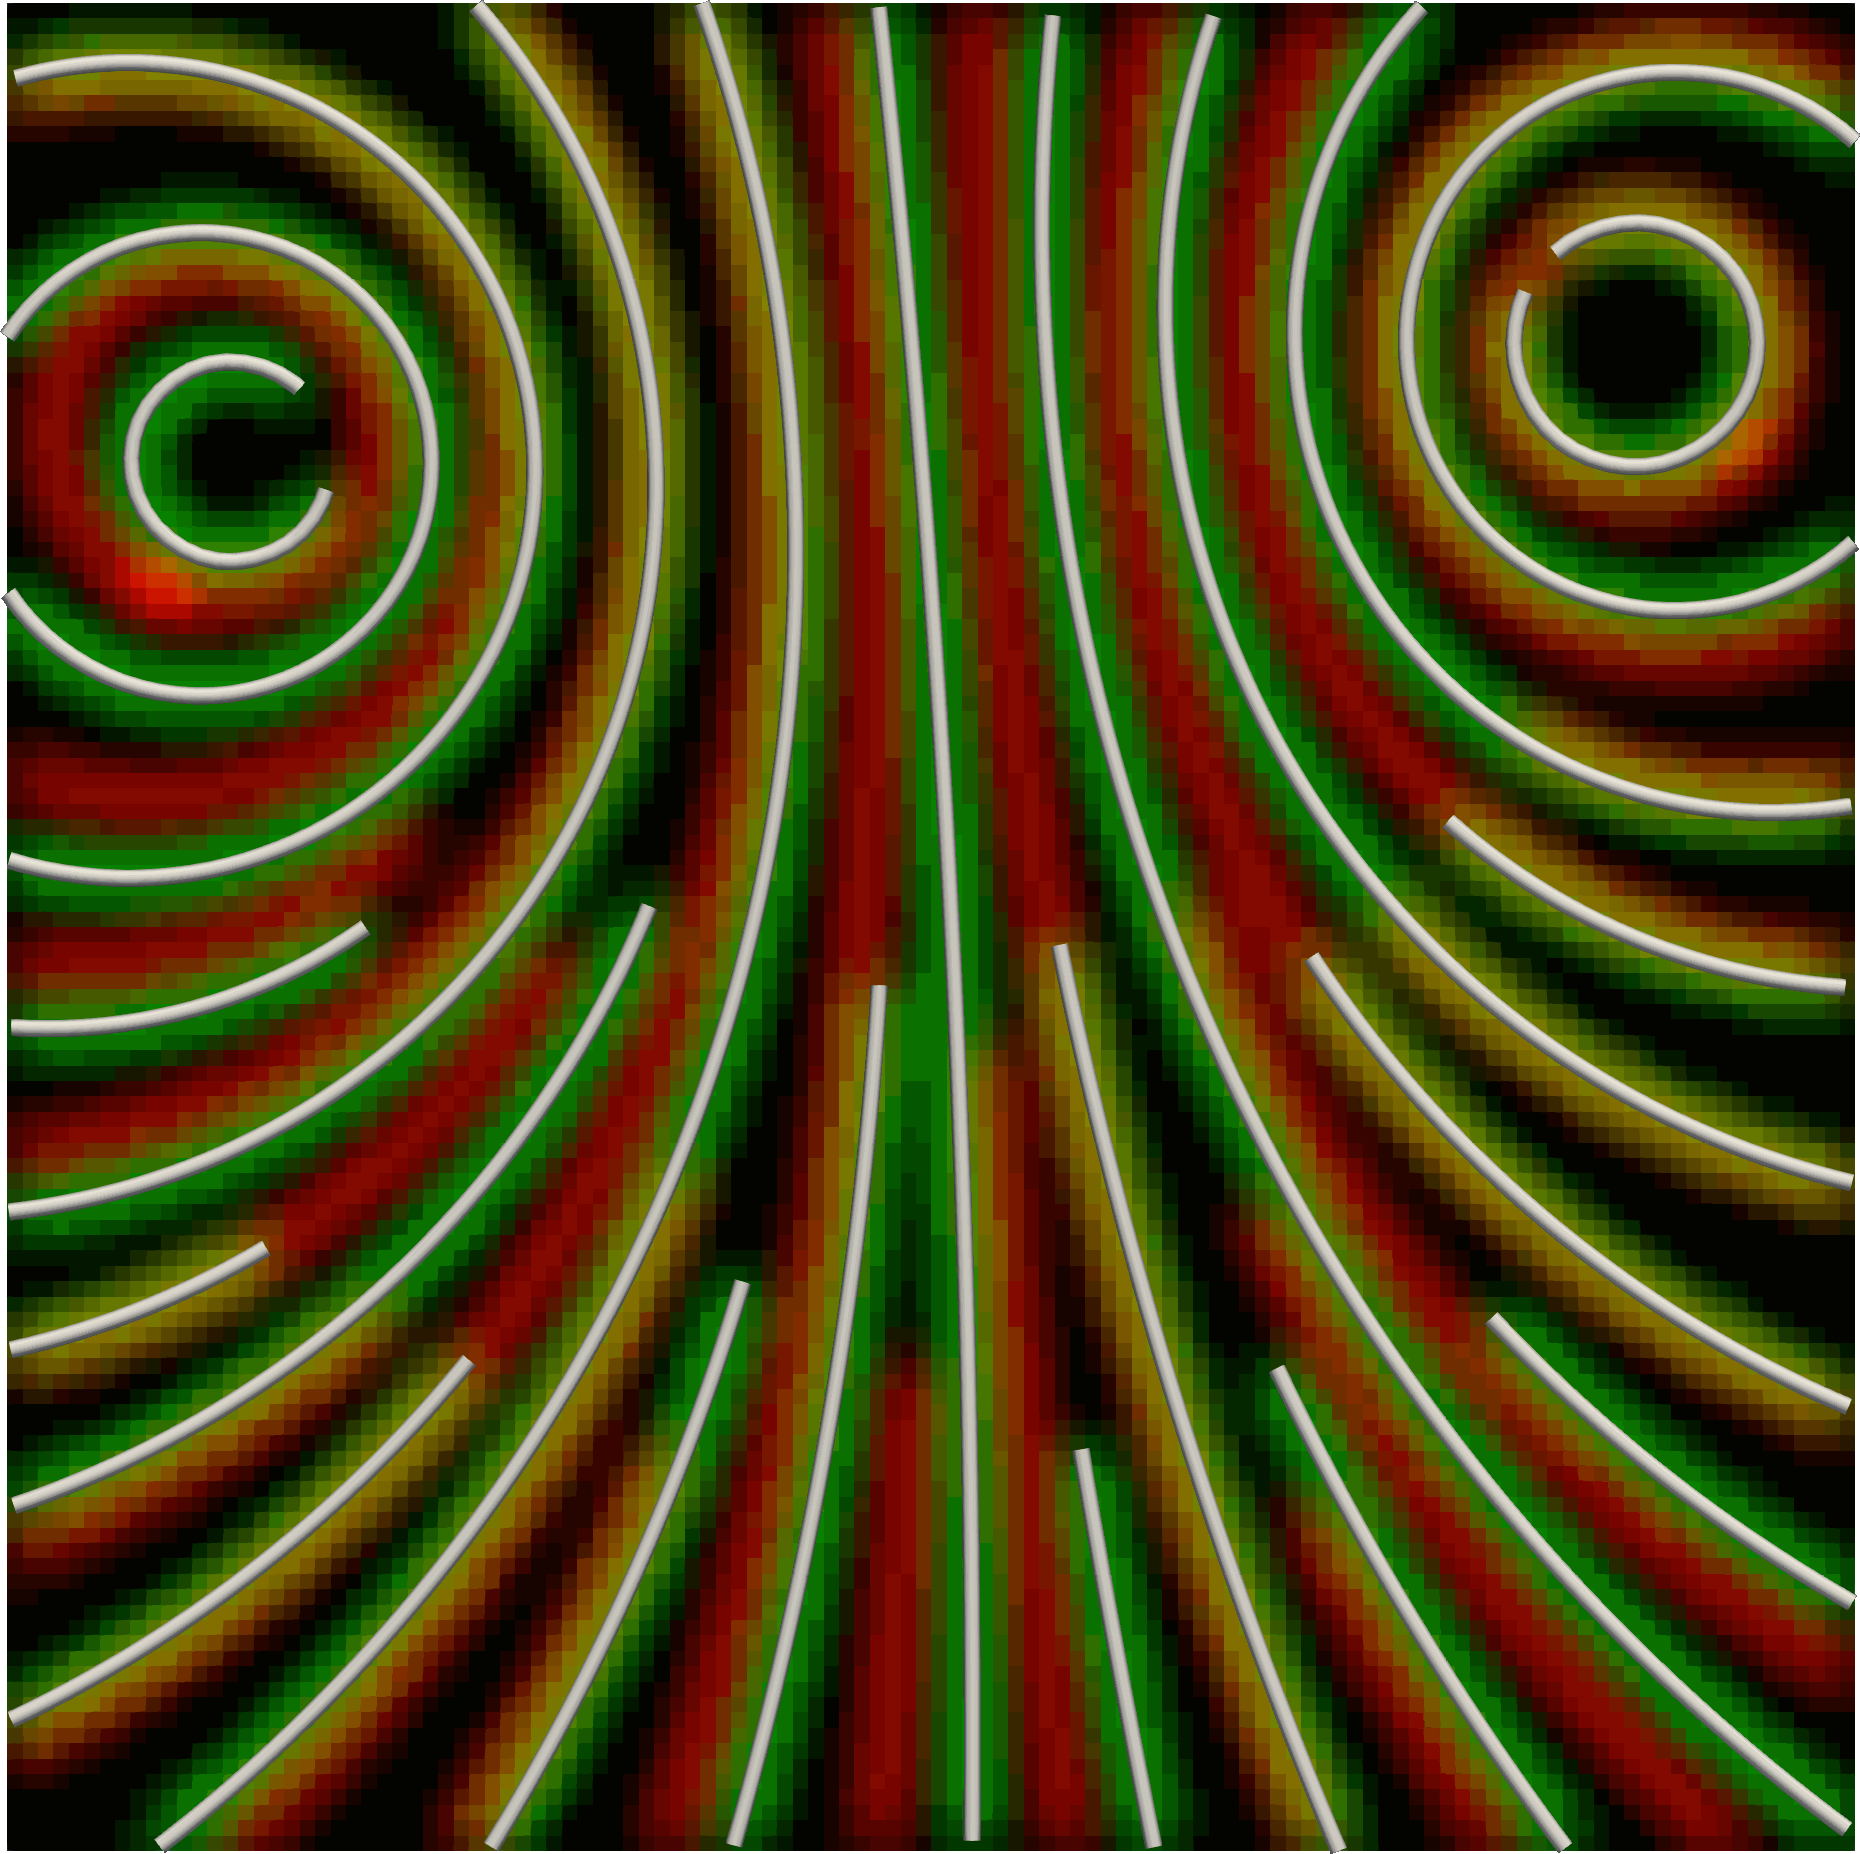
\includegraphics[scale=.055]{figures/AlphaStudy/GyroNC.0003.png}
        \end{subfigure}
        \begin{subfigure}{.19\textwidth}
            \centering
            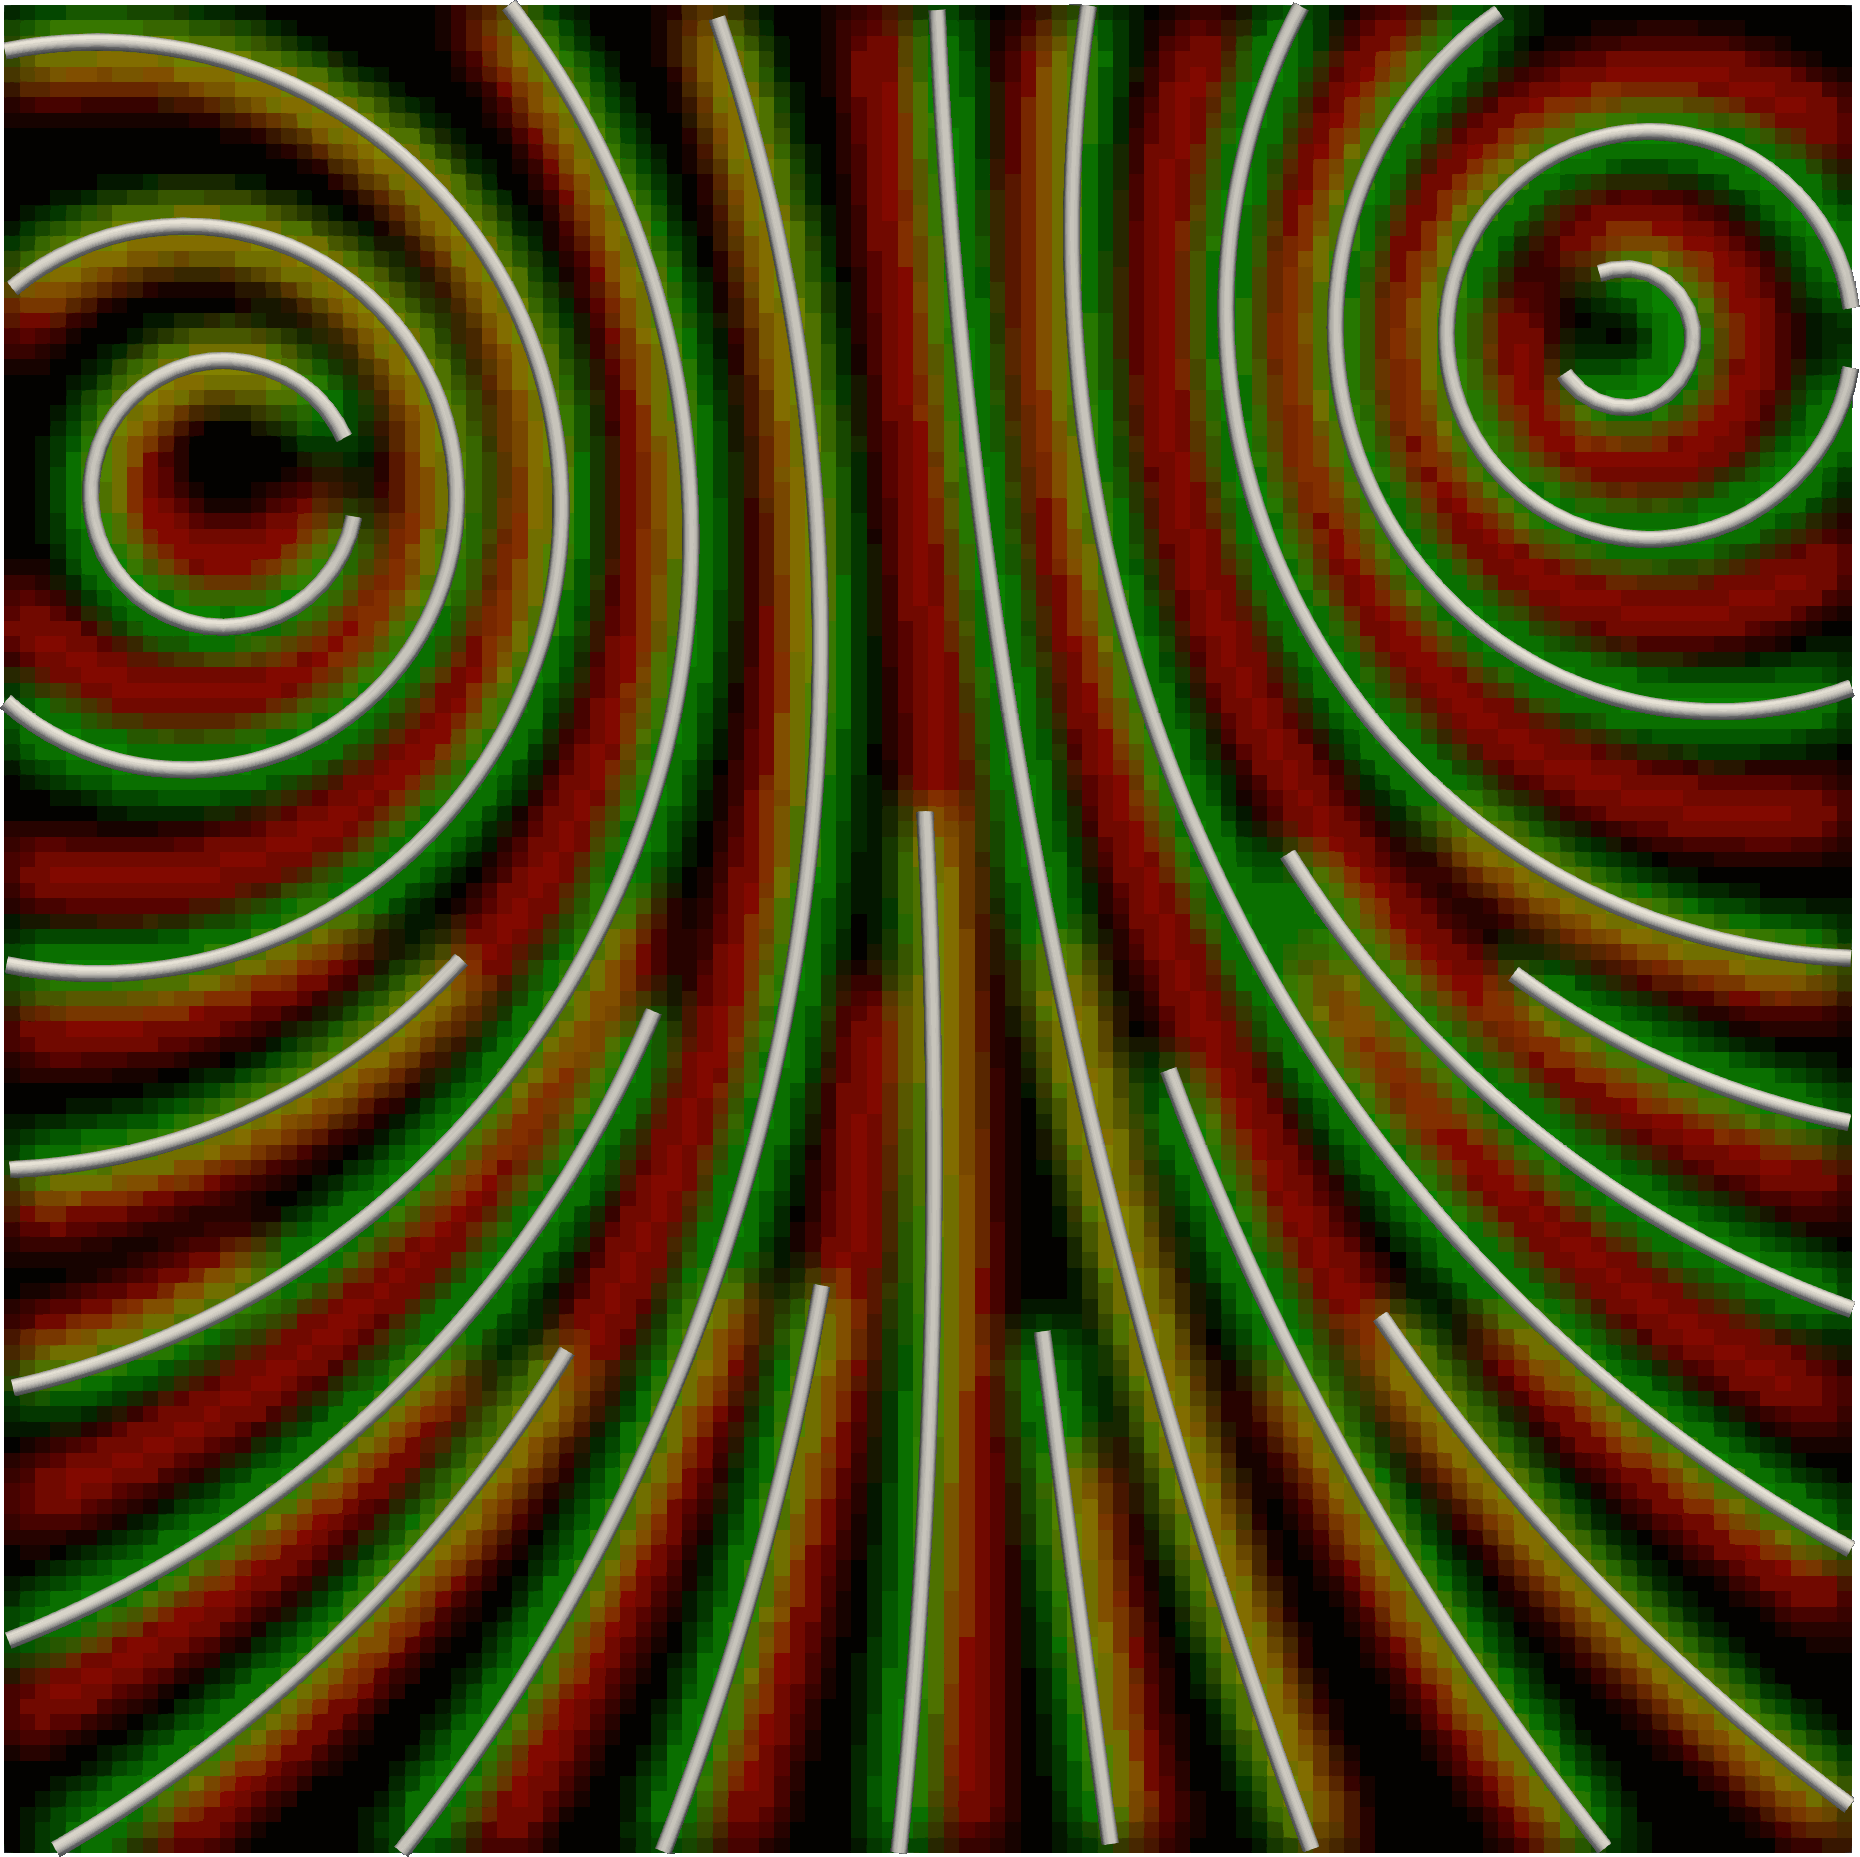
\includegraphics[scale=.055]{figures/AlphaStudy/GyroNC.0004.png}
        \end{subfigure}
        \caption*{(a)}
    \end{subfigure}
    % 5 x 1 / 3 coherence
    \begin{subfigure}{\textwidth}
        \begin{subfigure}{.19\textwidth}
            \centering
            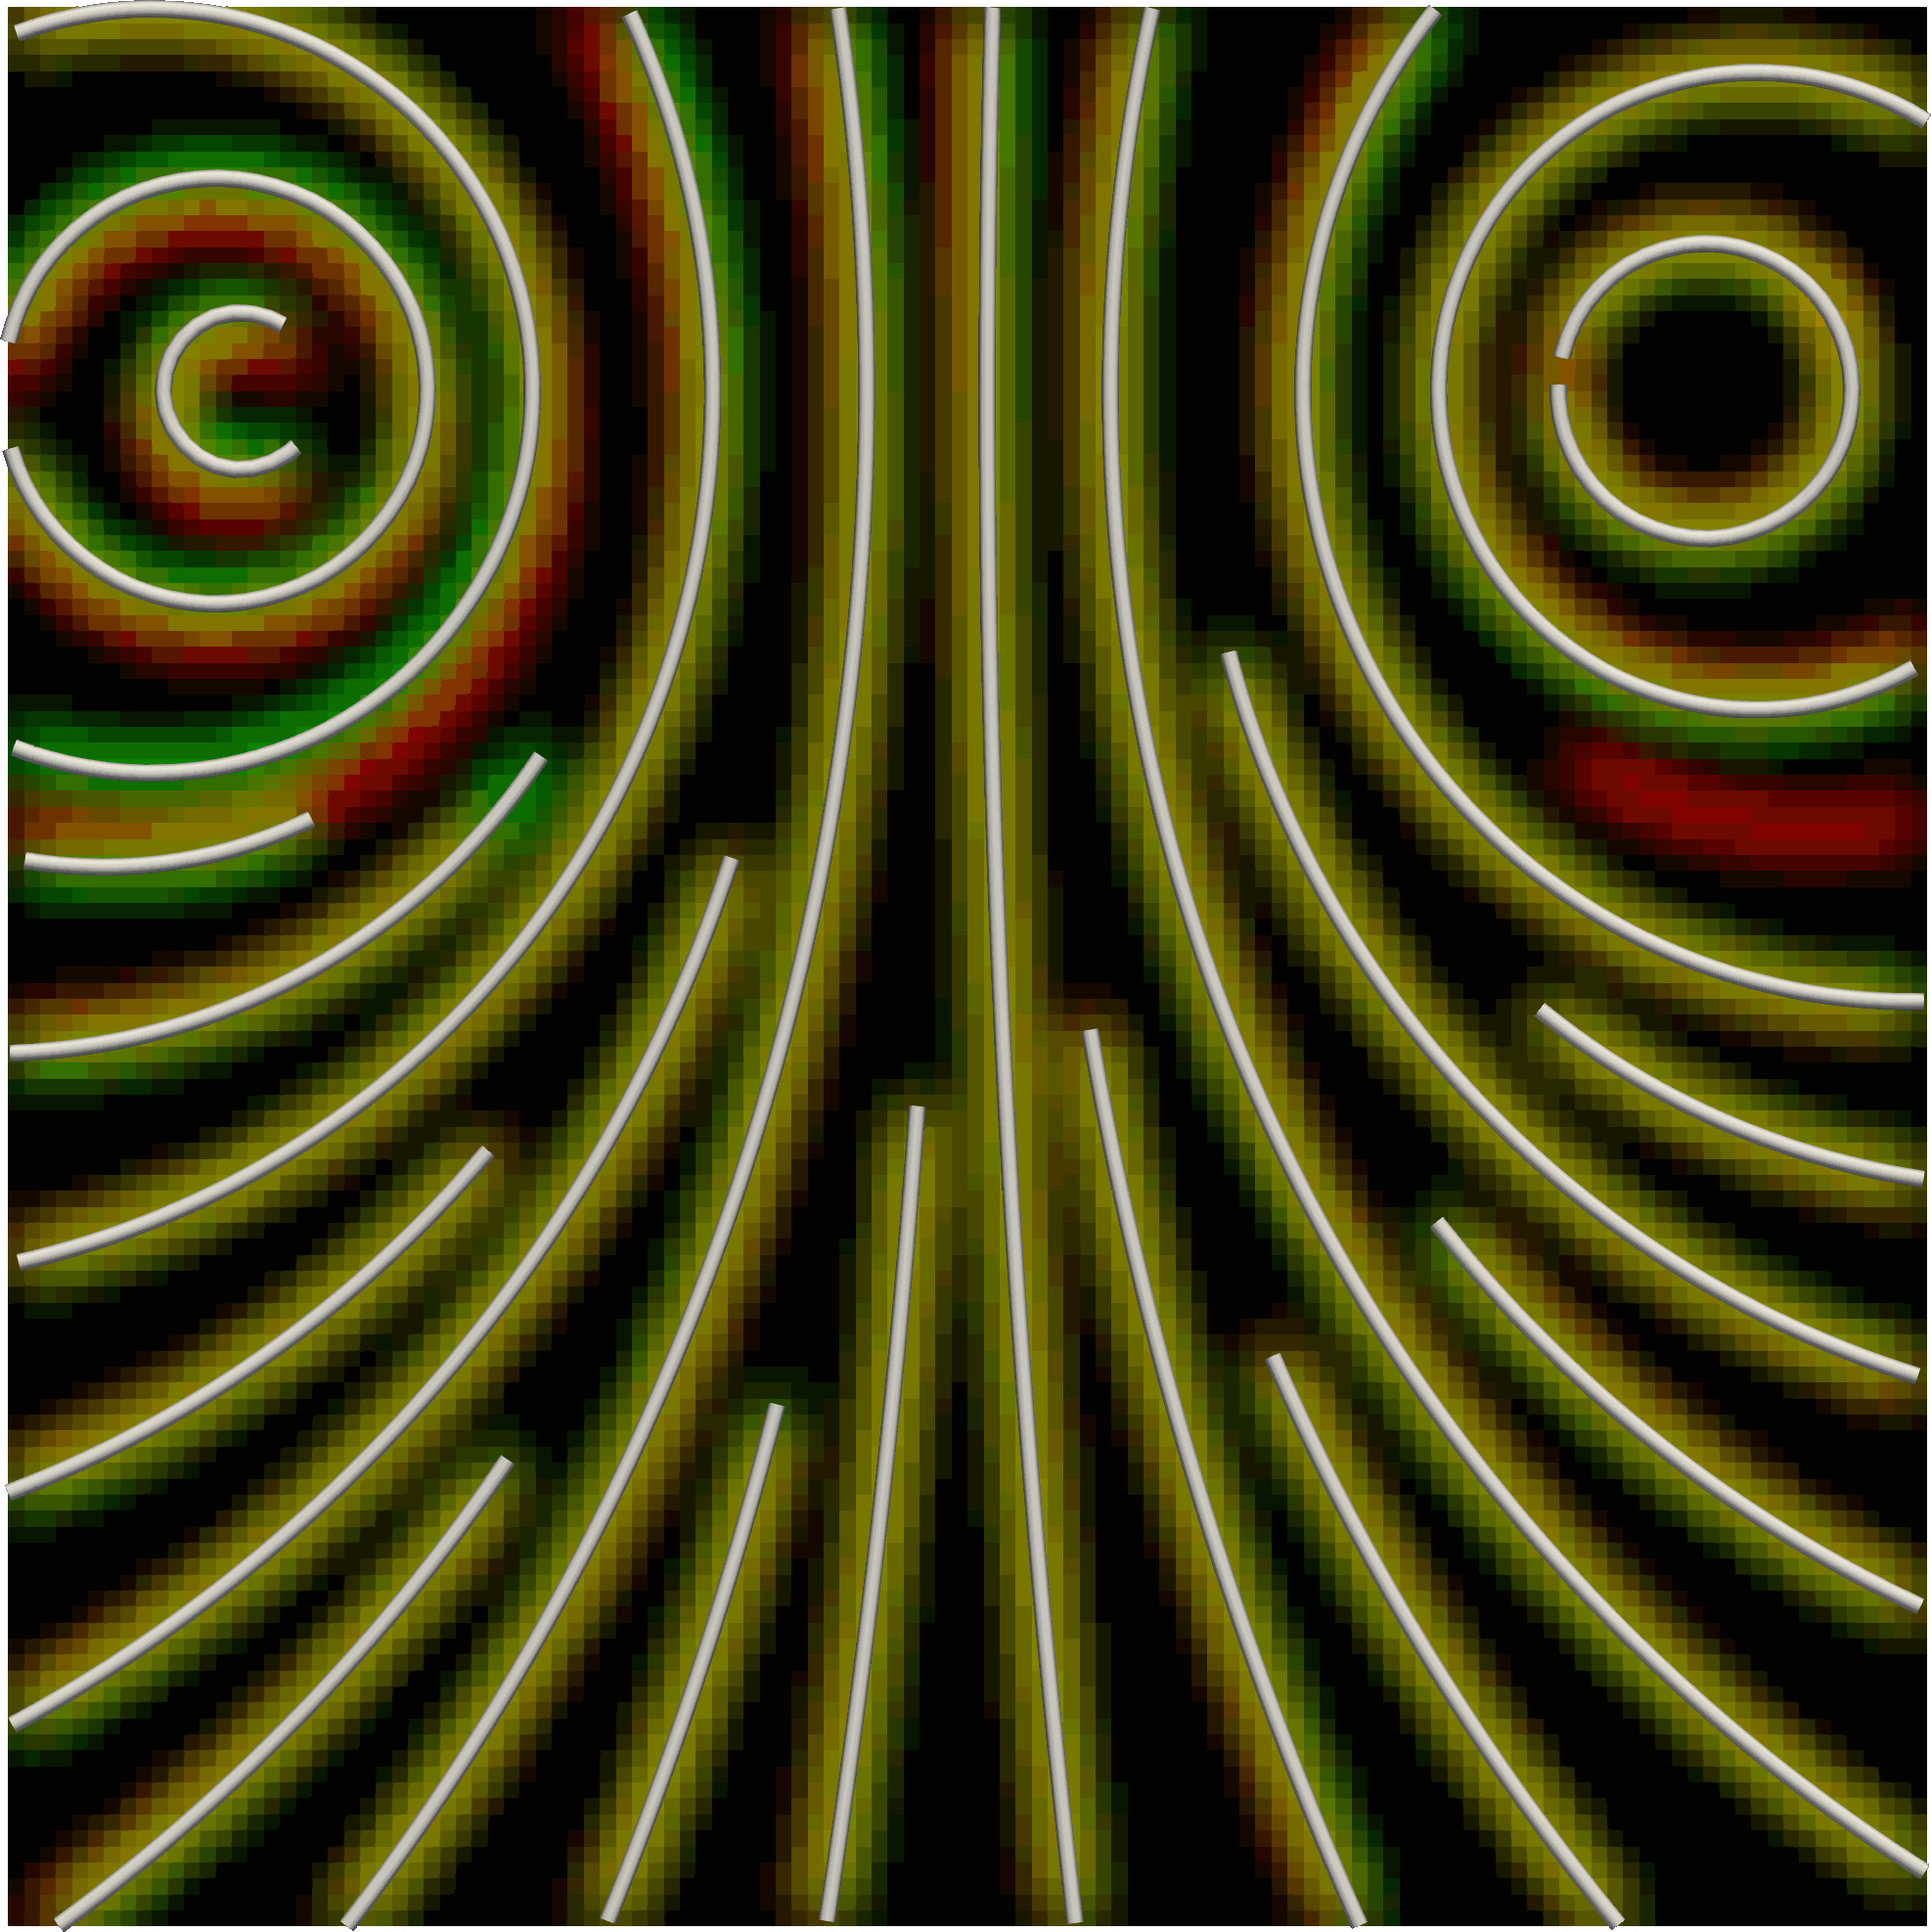
\includegraphics[scale=.0515]{figures/AlphaStudy/Gyro13C.0000.png}
        \end{subfigure}
        \begin{subfigure}{.19\textwidth}
            \centering
            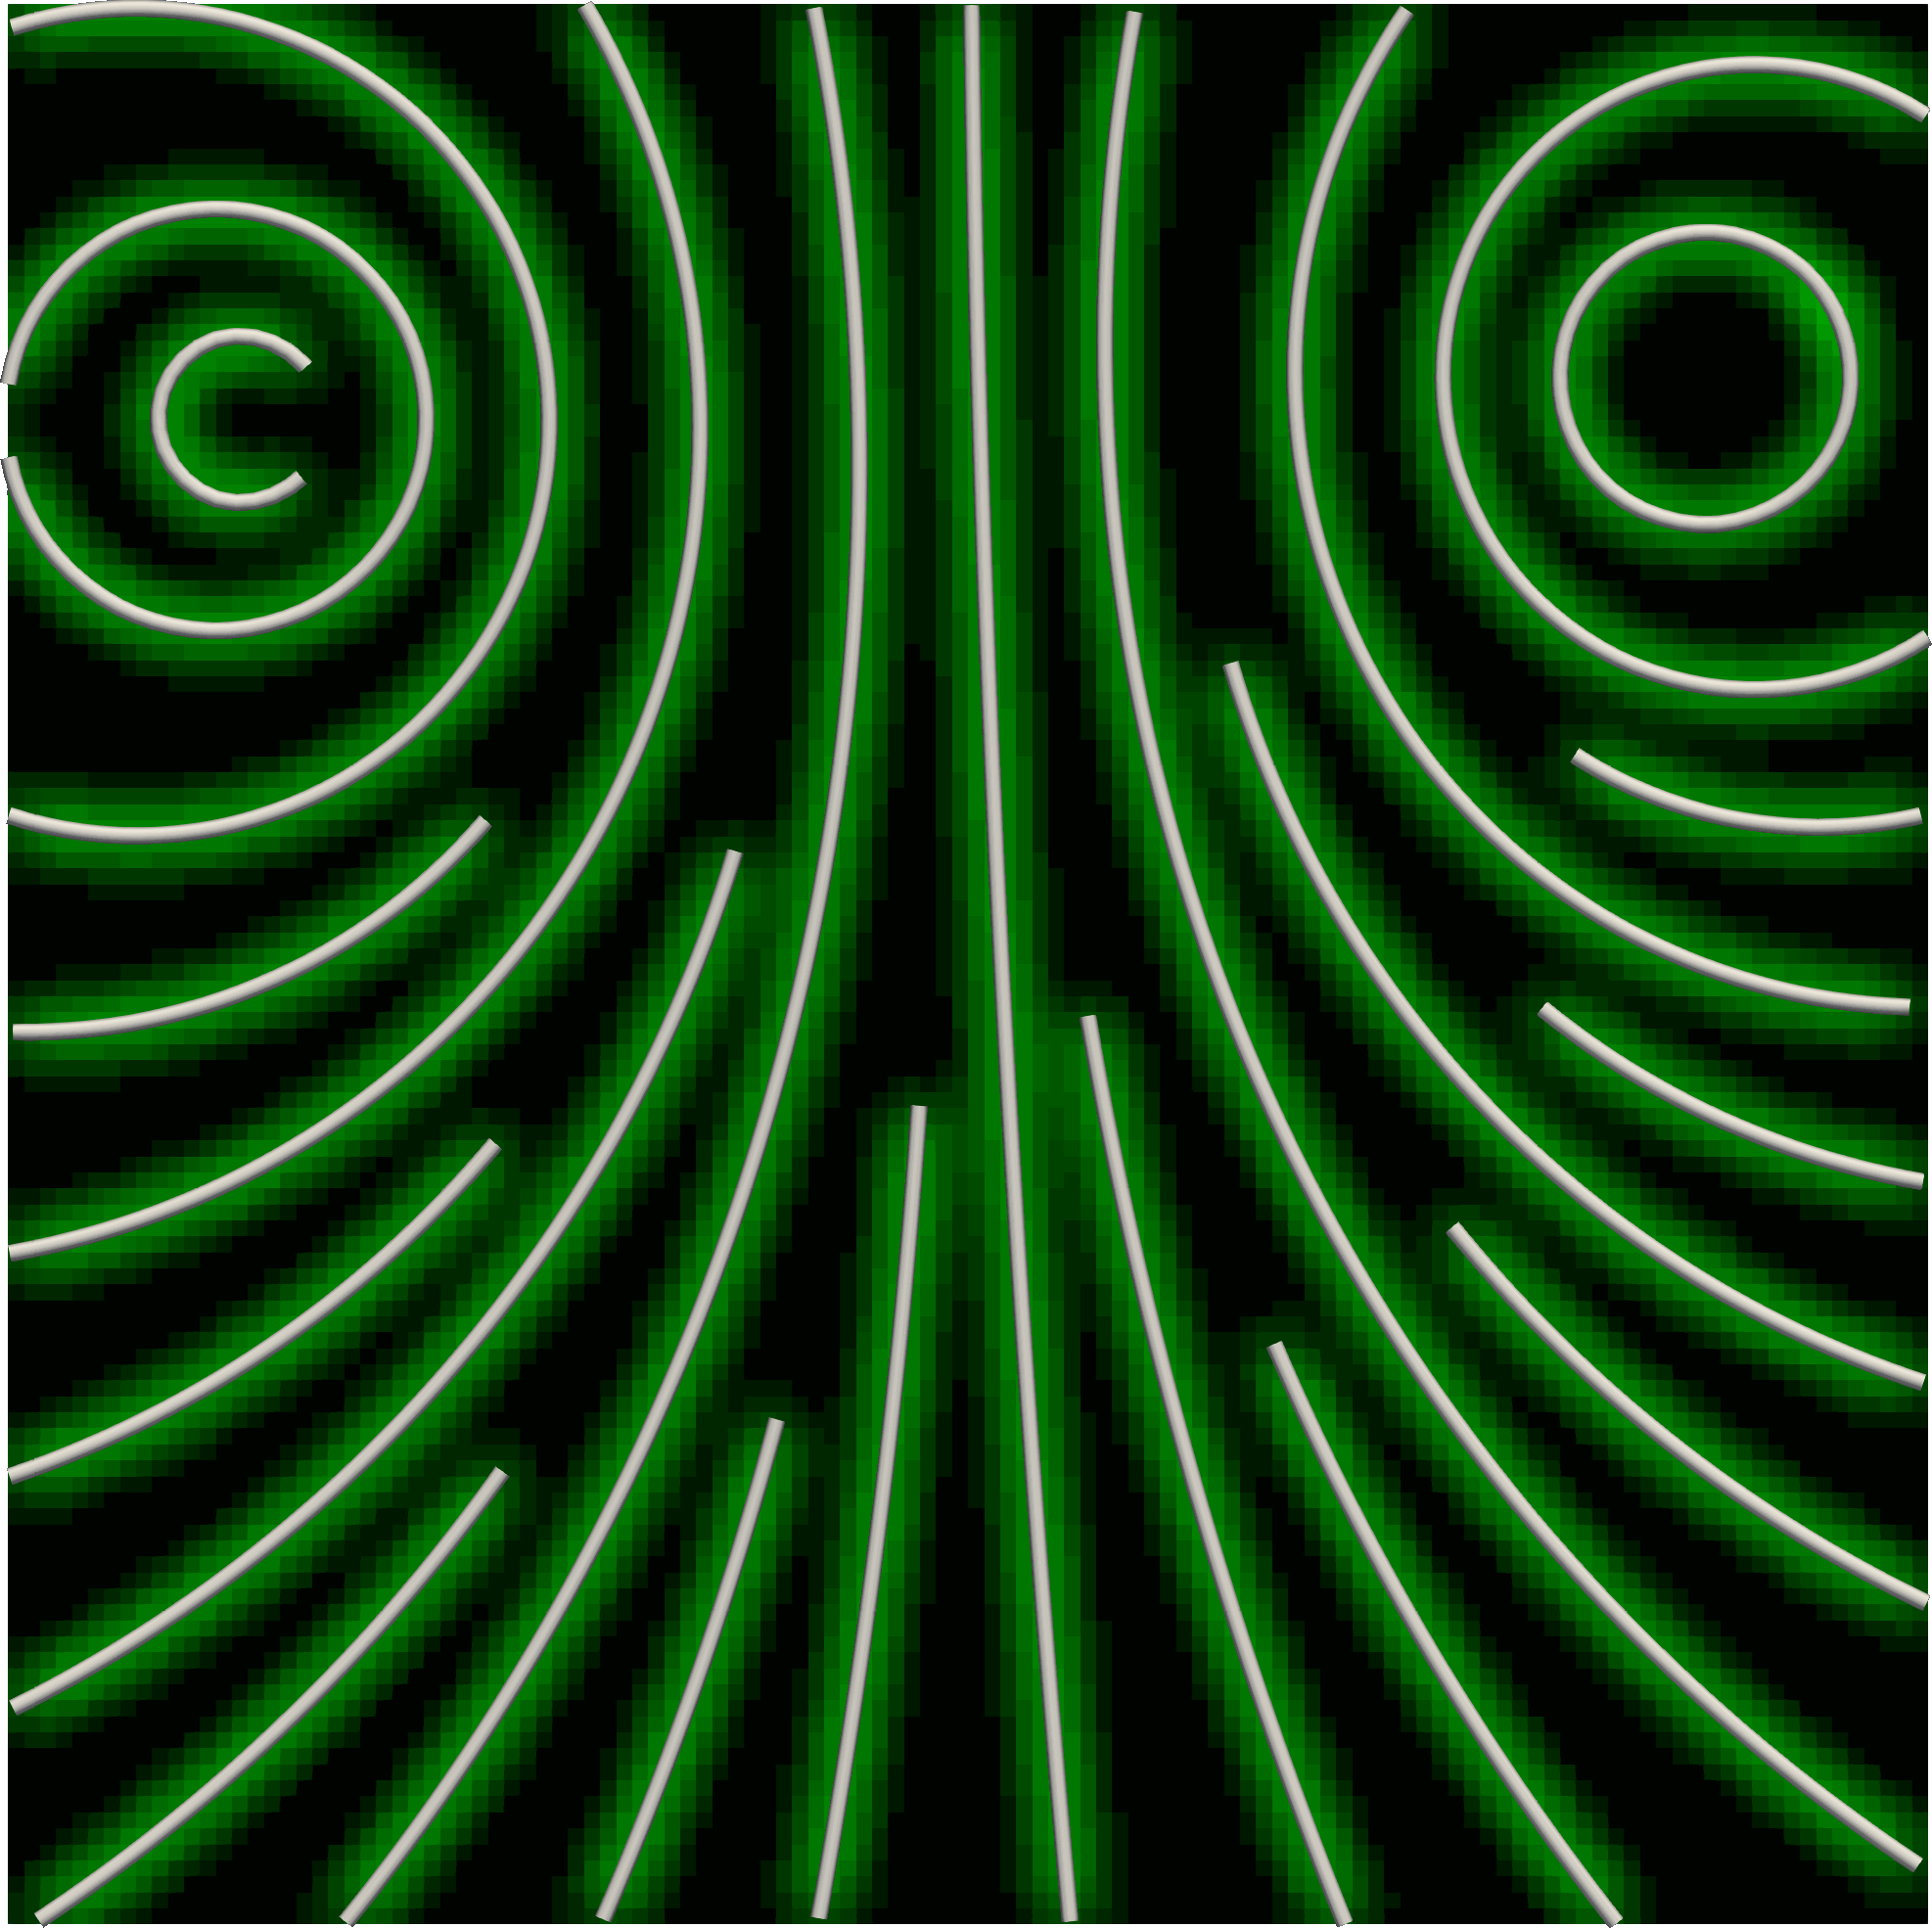
\includegraphics[scale=.0515]{figures/AlphaStudy/Gyro13C.0001.png}
        \end{subfigure}
        \begin{subfigure}{.19\textwidth}
            \centering
            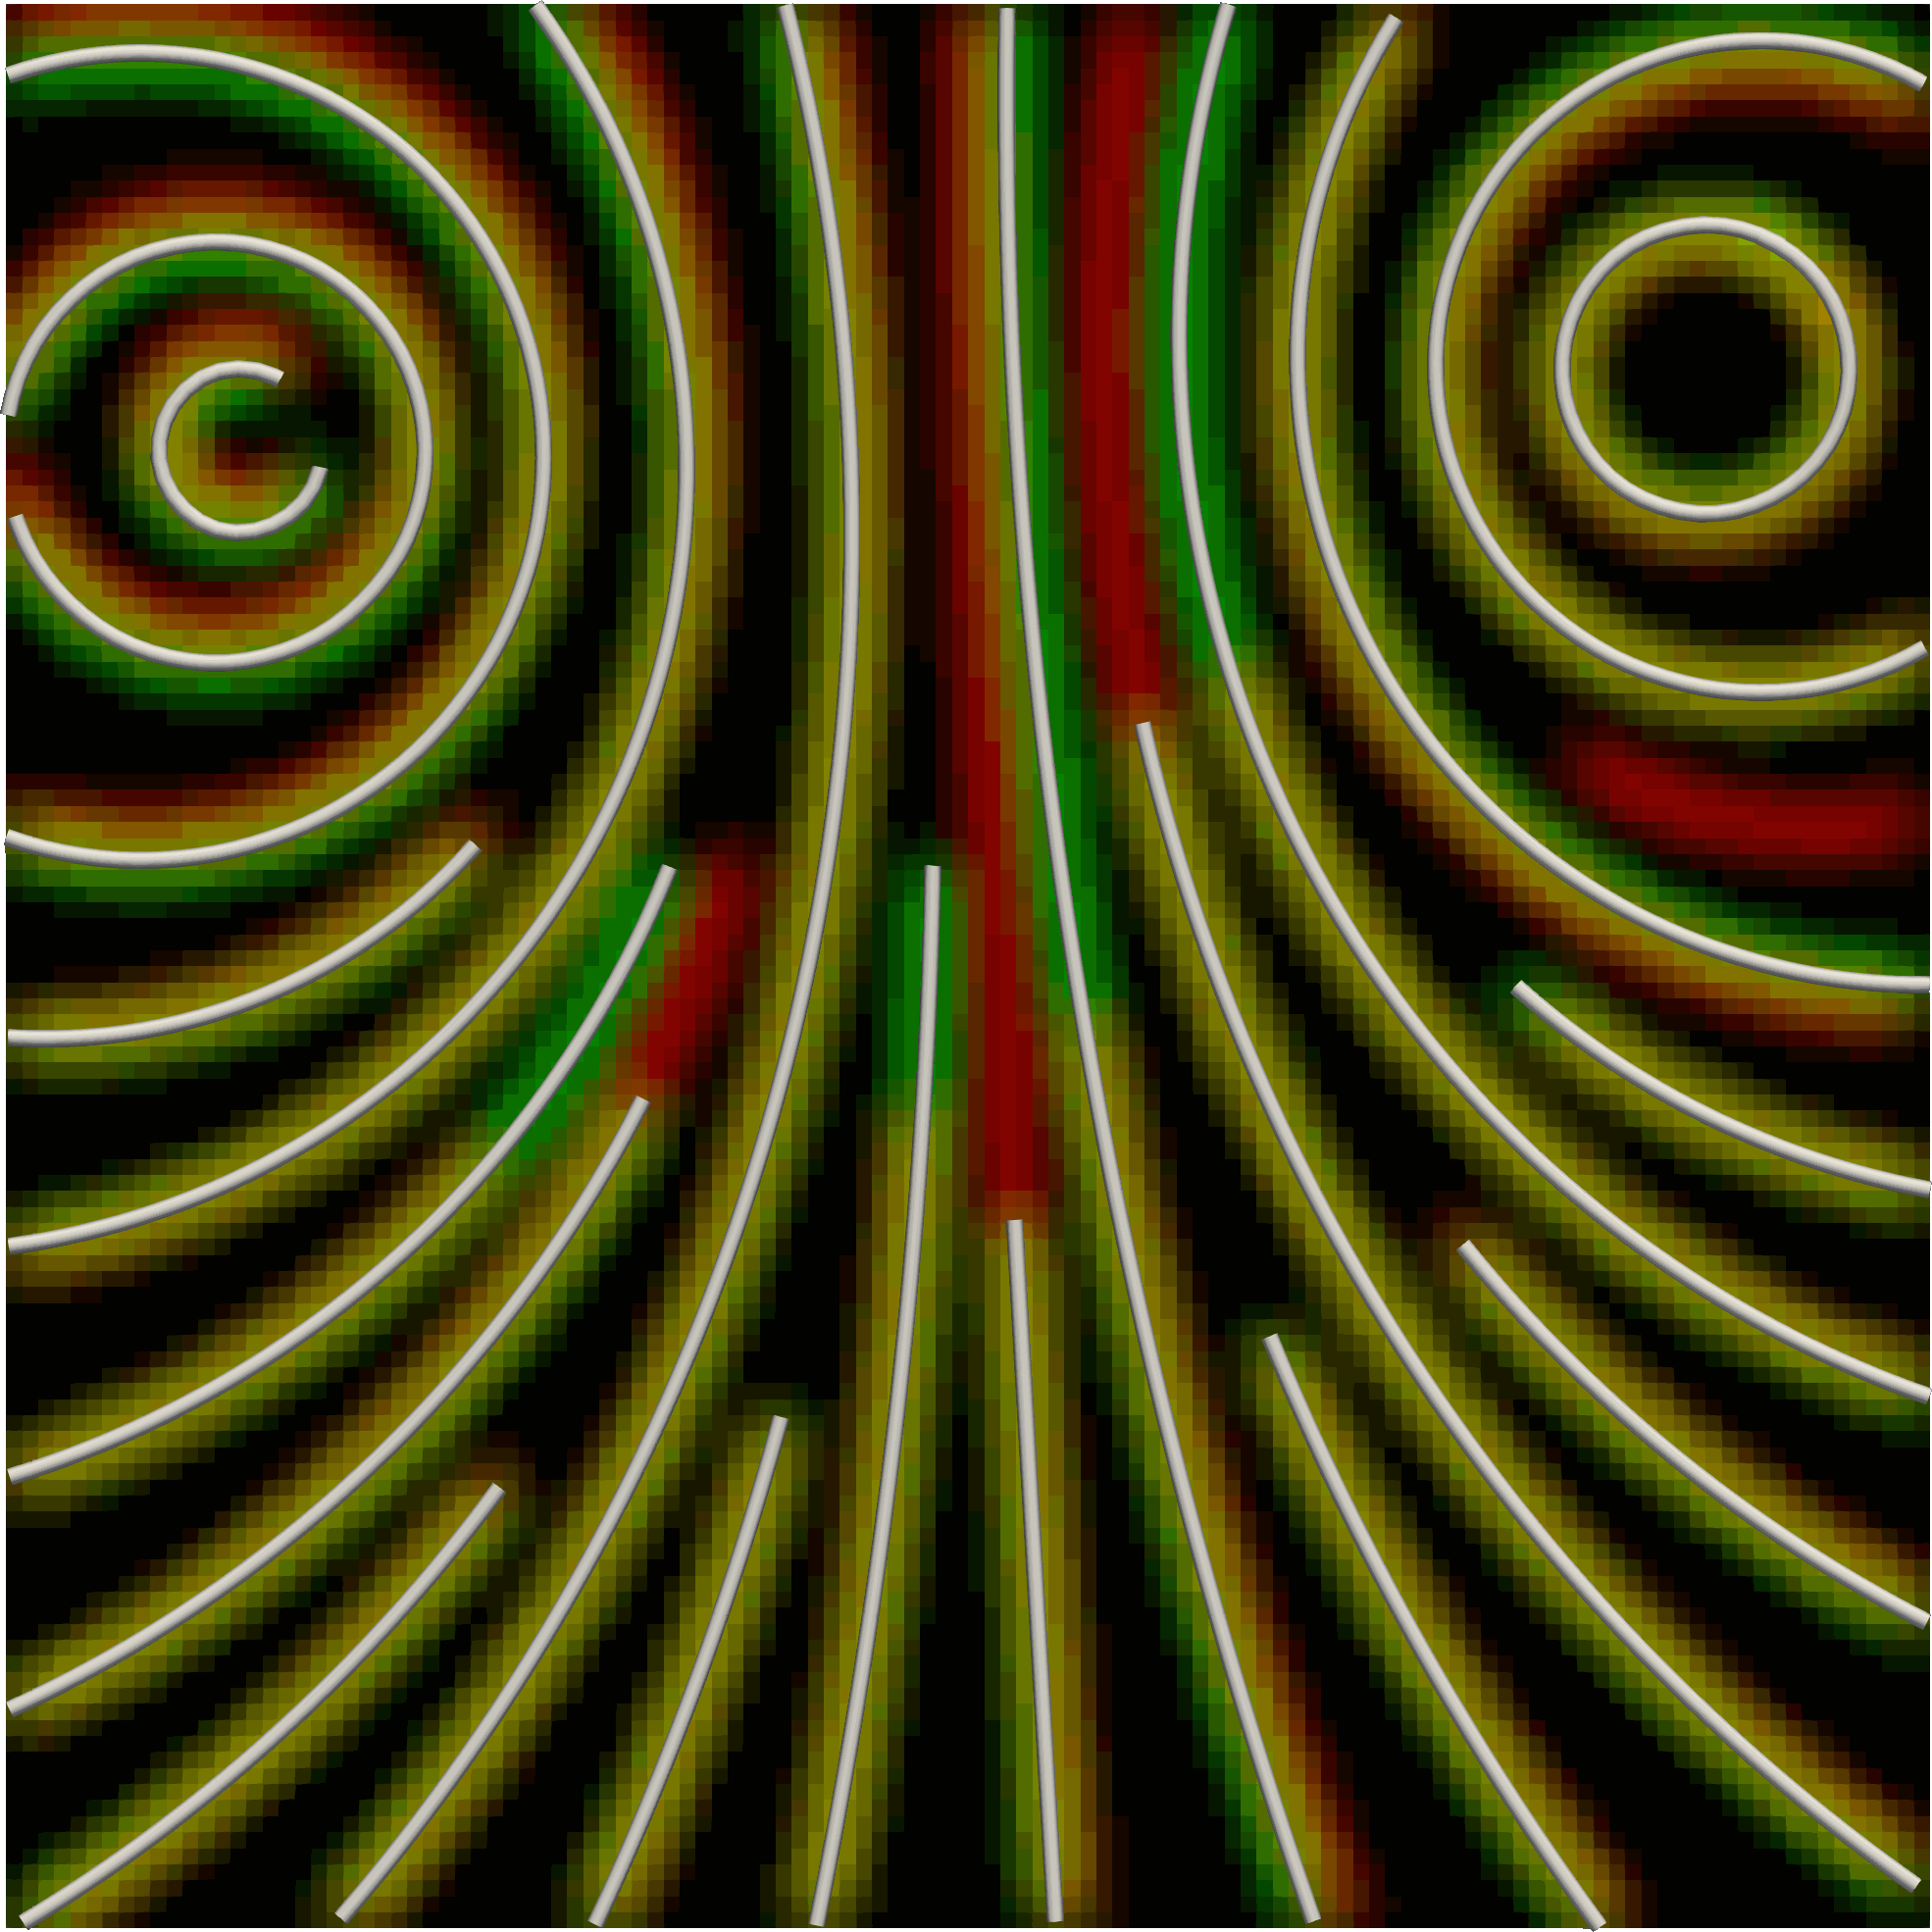
\includegraphics[scale=.0515]{figures/AlphaStudy/Gyro13C.0002.png}
        \end{subfigure}
        \begin{subfigure}{.19\textwidth}
            \centering
            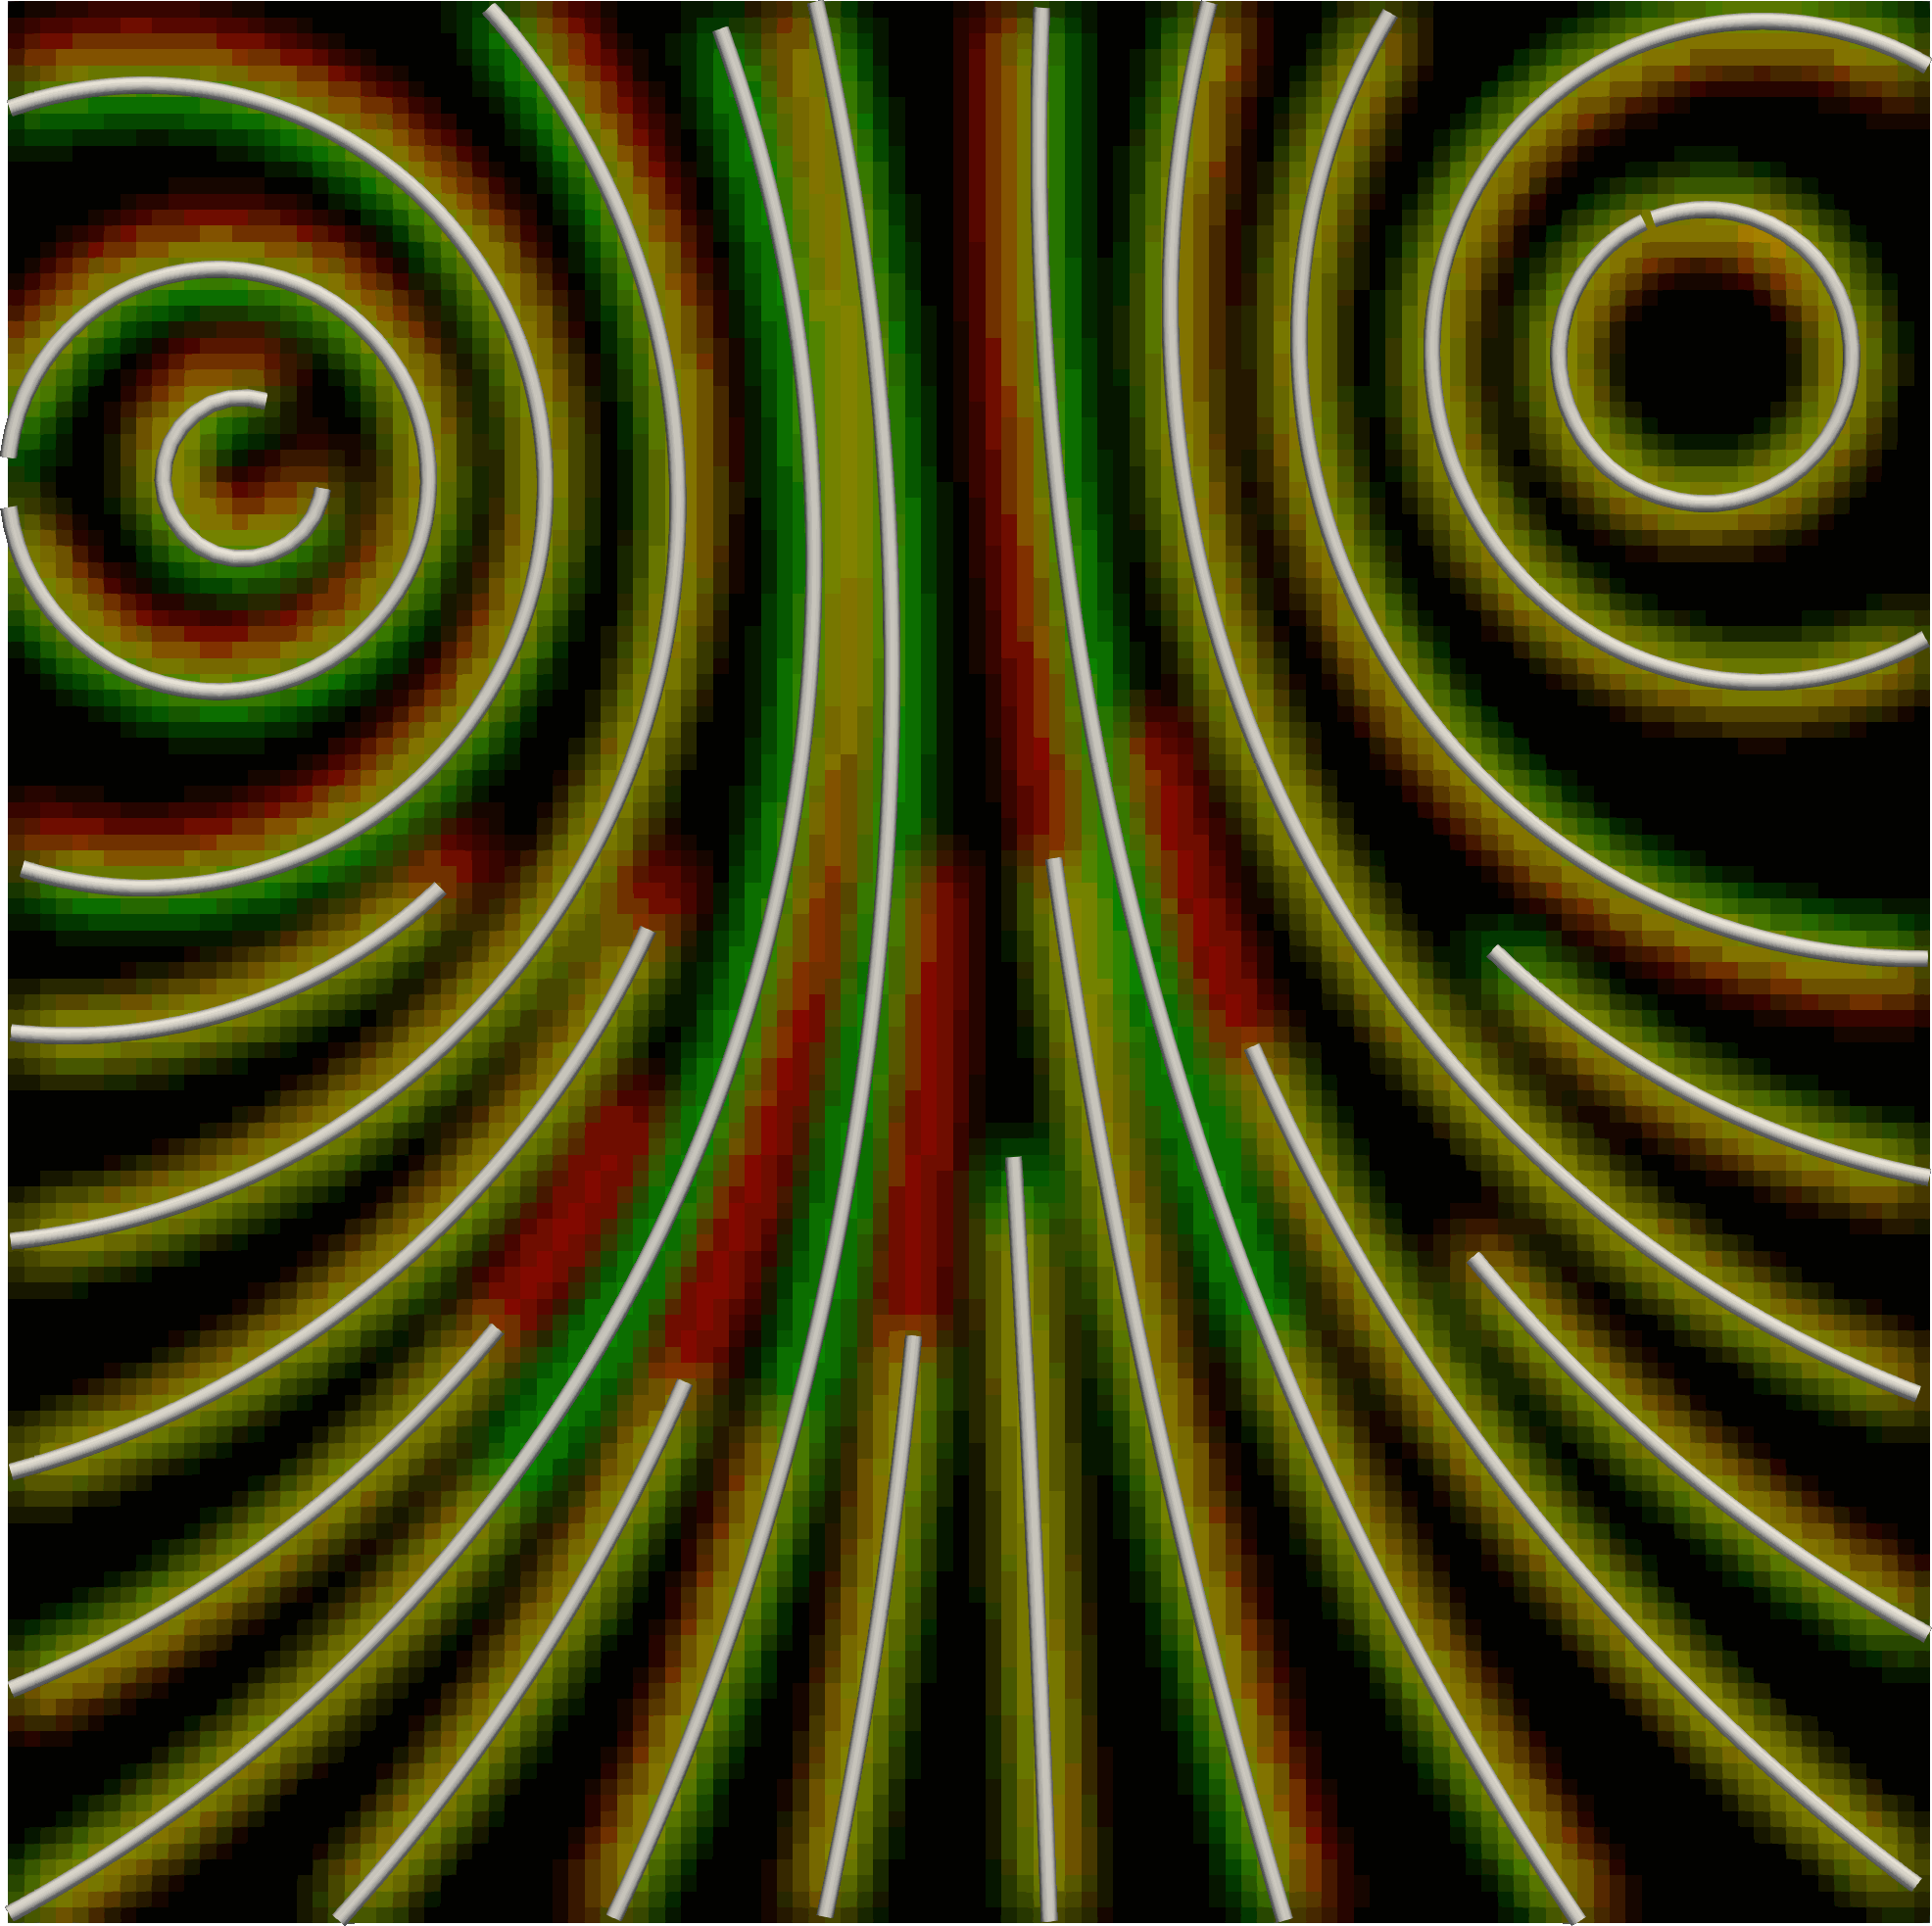
\includegraphics[scale=.0515]{figures/AlphaStudy/Gyro13C.0003.png}
        \end{subfigure}
        \begin{subfigure}{.19\textwidth}
            \centering
            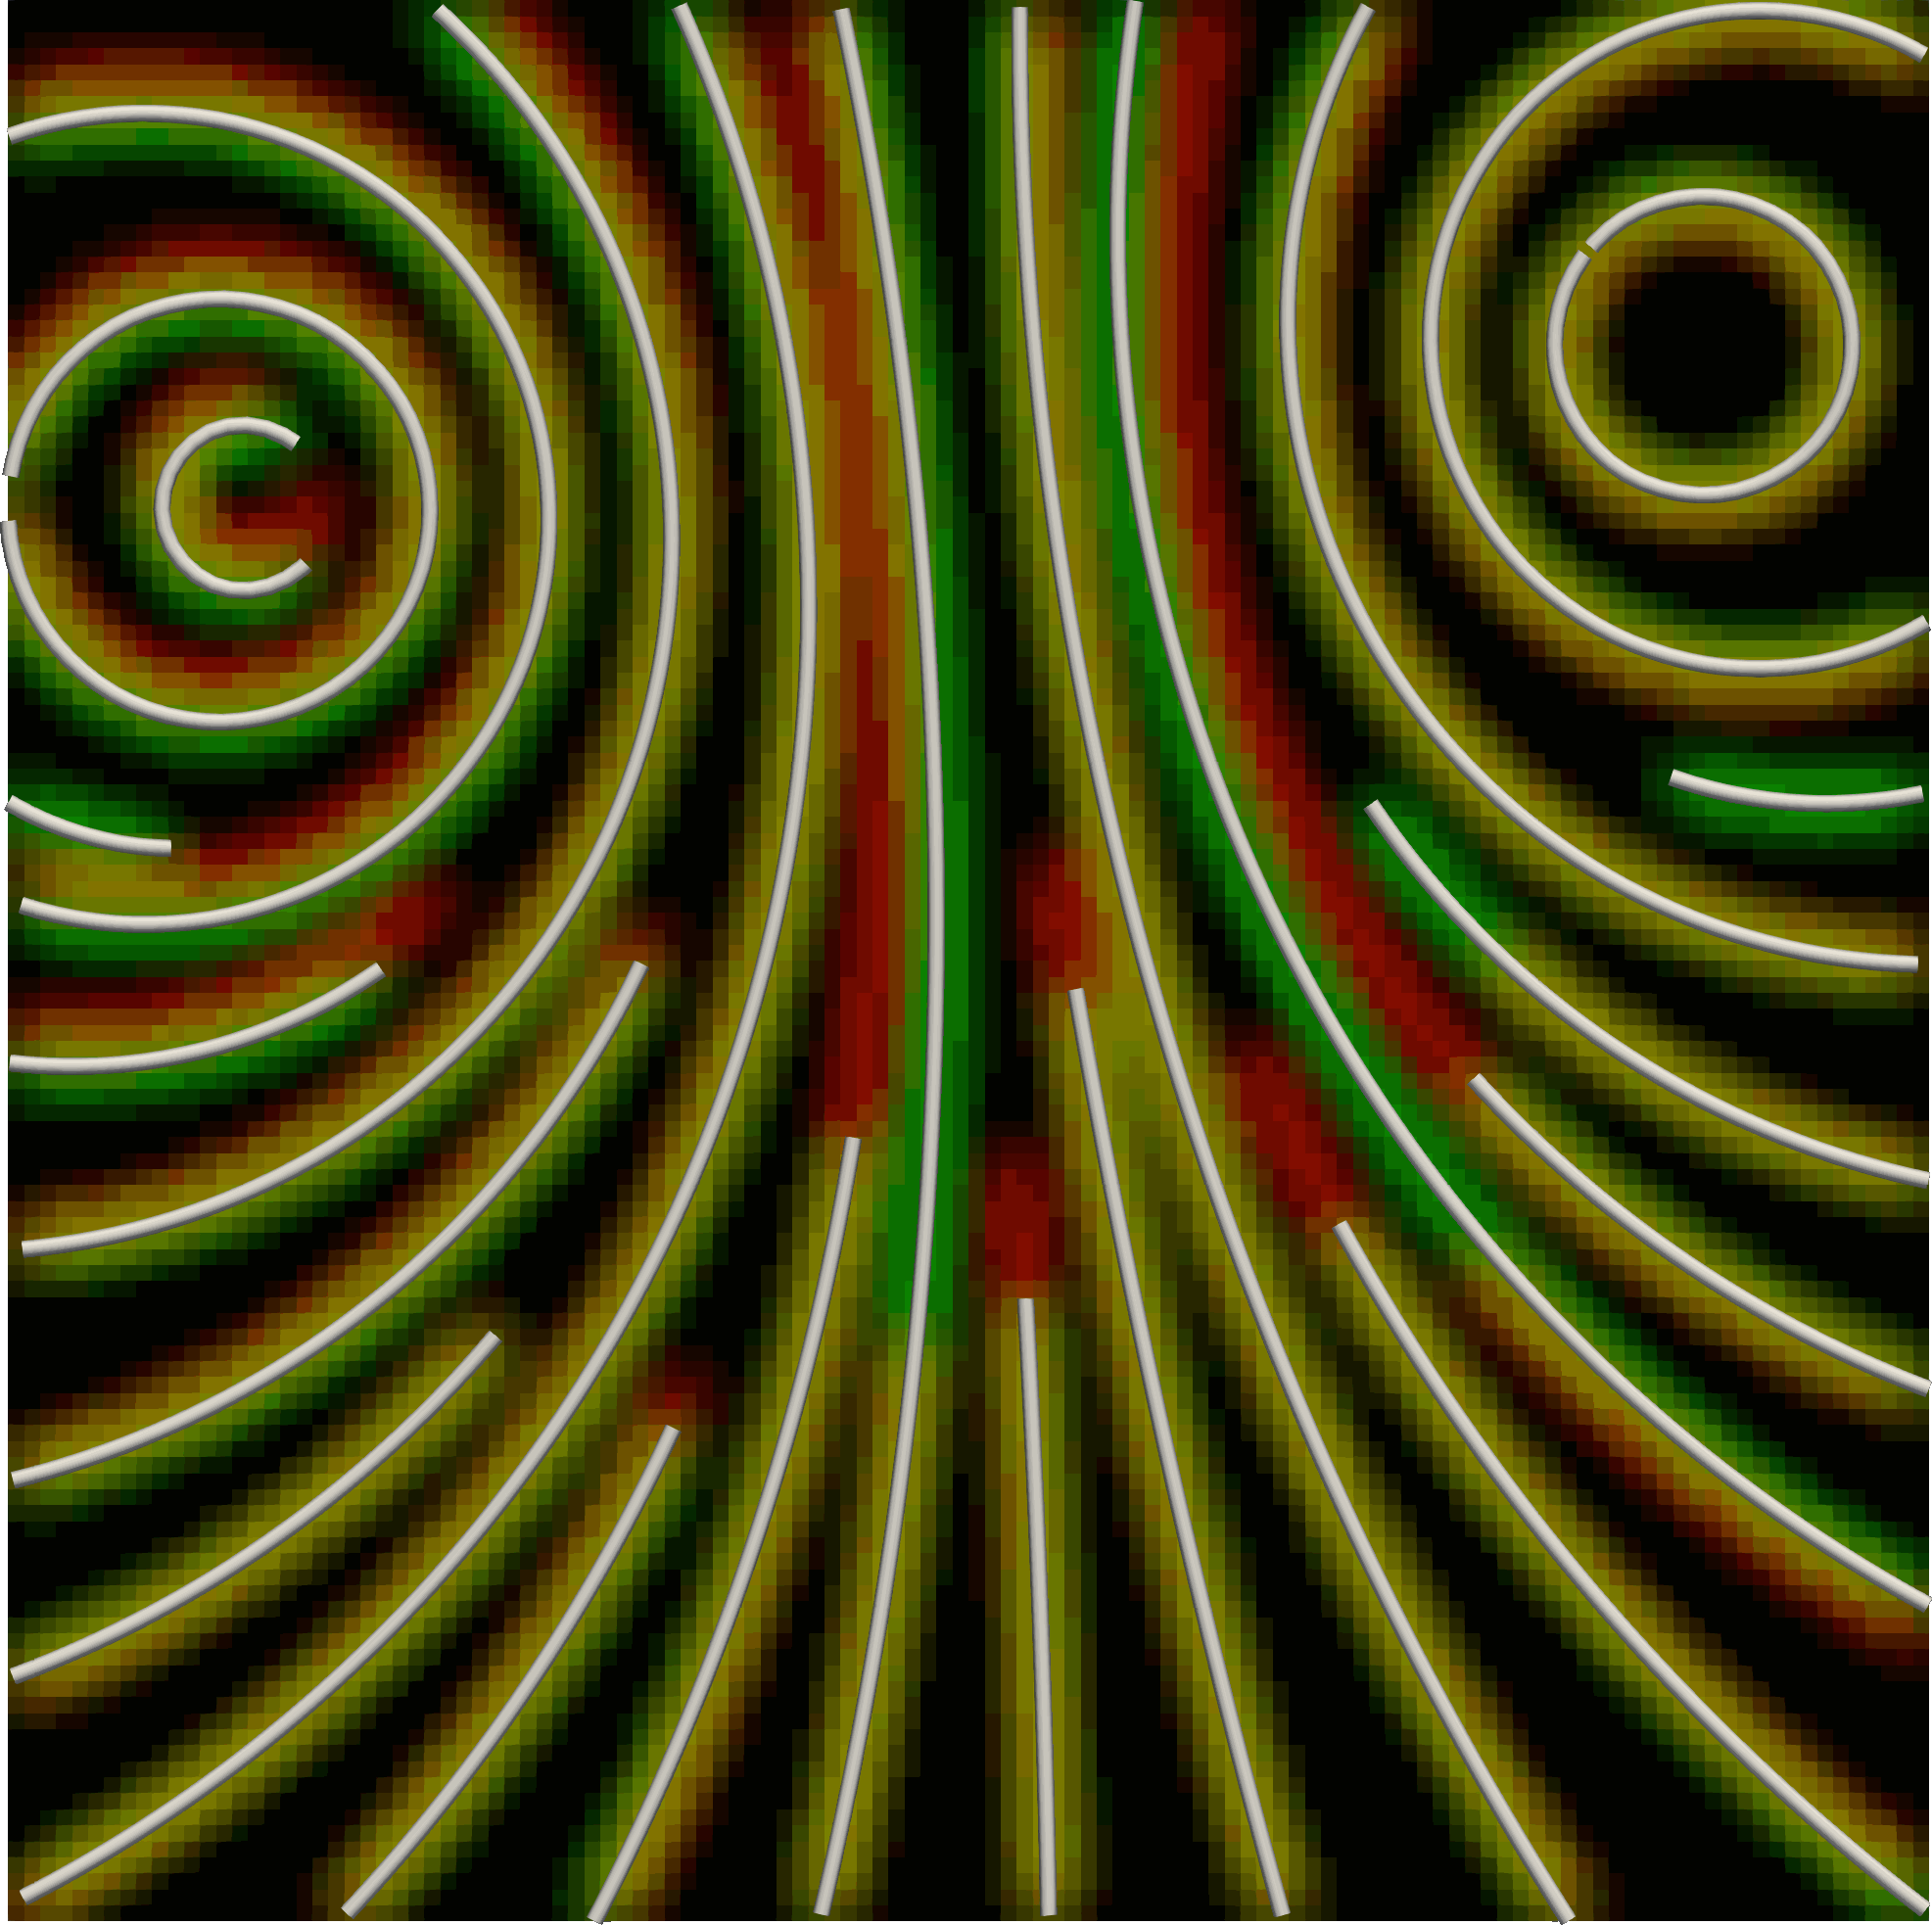
\includegraphics[scale=.0515]{figures/AlphaStudy/Gyro13C.0004.png}
        \end{subfigure}
        \caption*{(b)}
    \end{subfigure}
    % 5 x 2 / 3 coherence
    \begin{subfigure}{\textwidth}
        \begin{subfigure}{.19\textwidth}
            \centering
            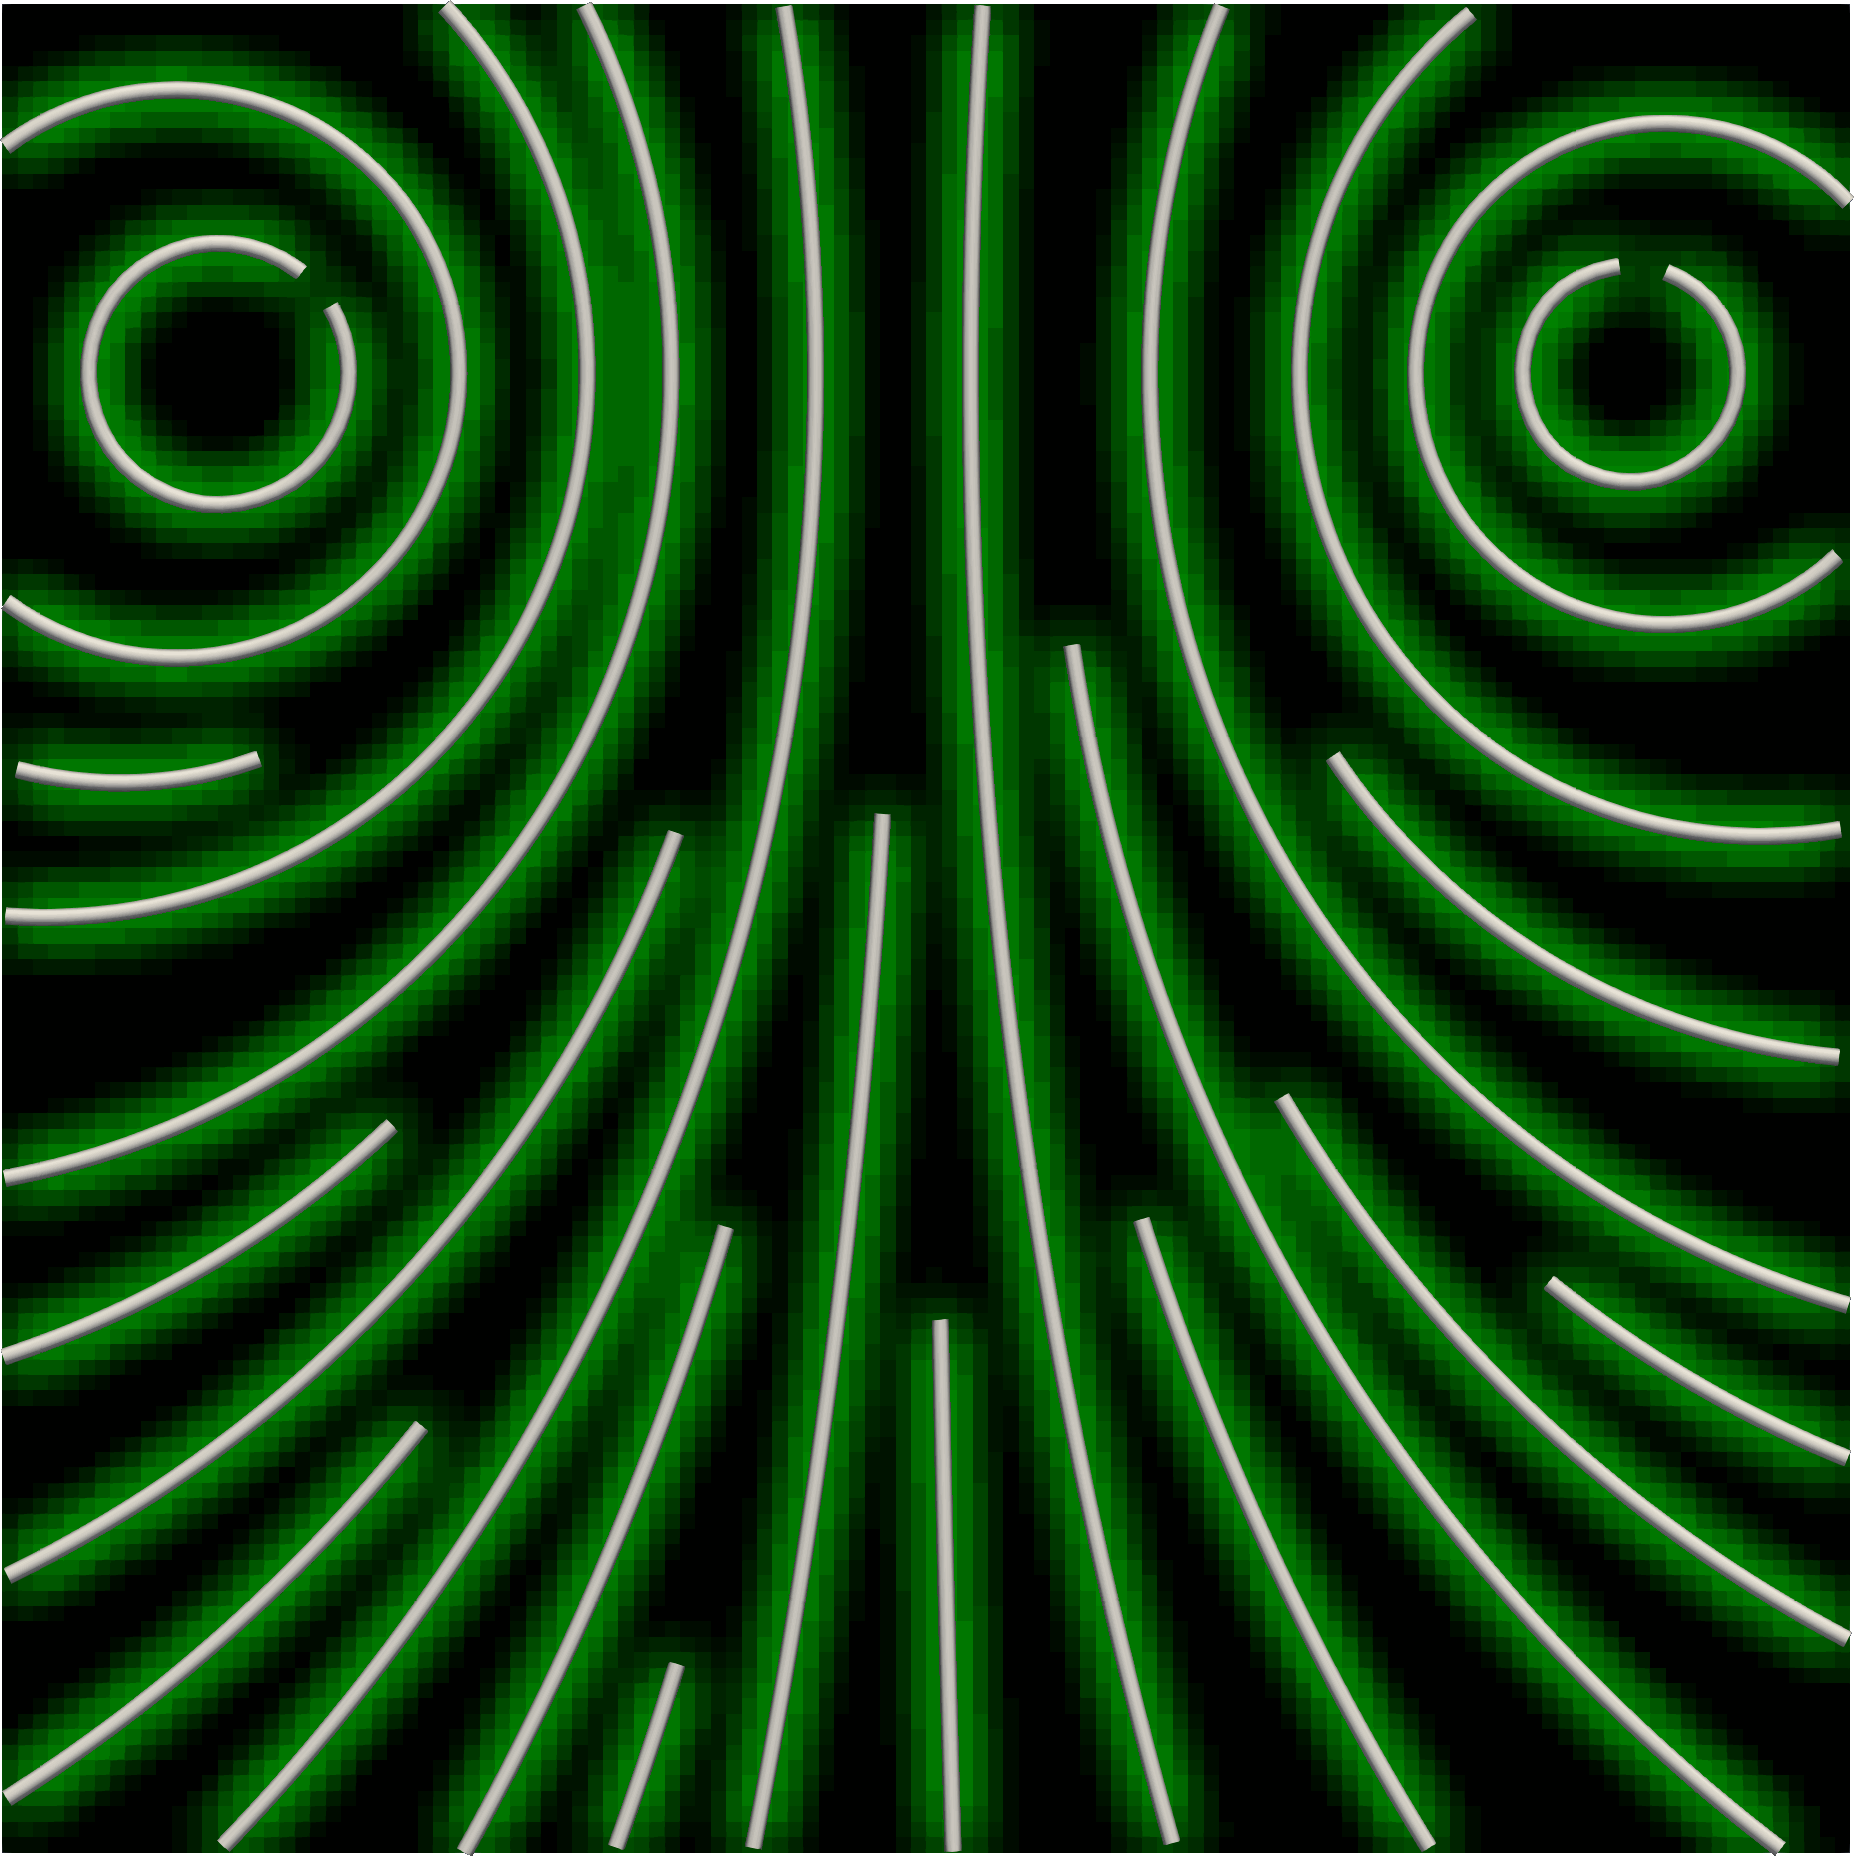
\includegraphics[scale=.055]{figures/AlphaStudy/Gyro23C.0000.png}
        \end{subfigure}
        \begin{subfigure}{.19\textwidth}
            \centering
            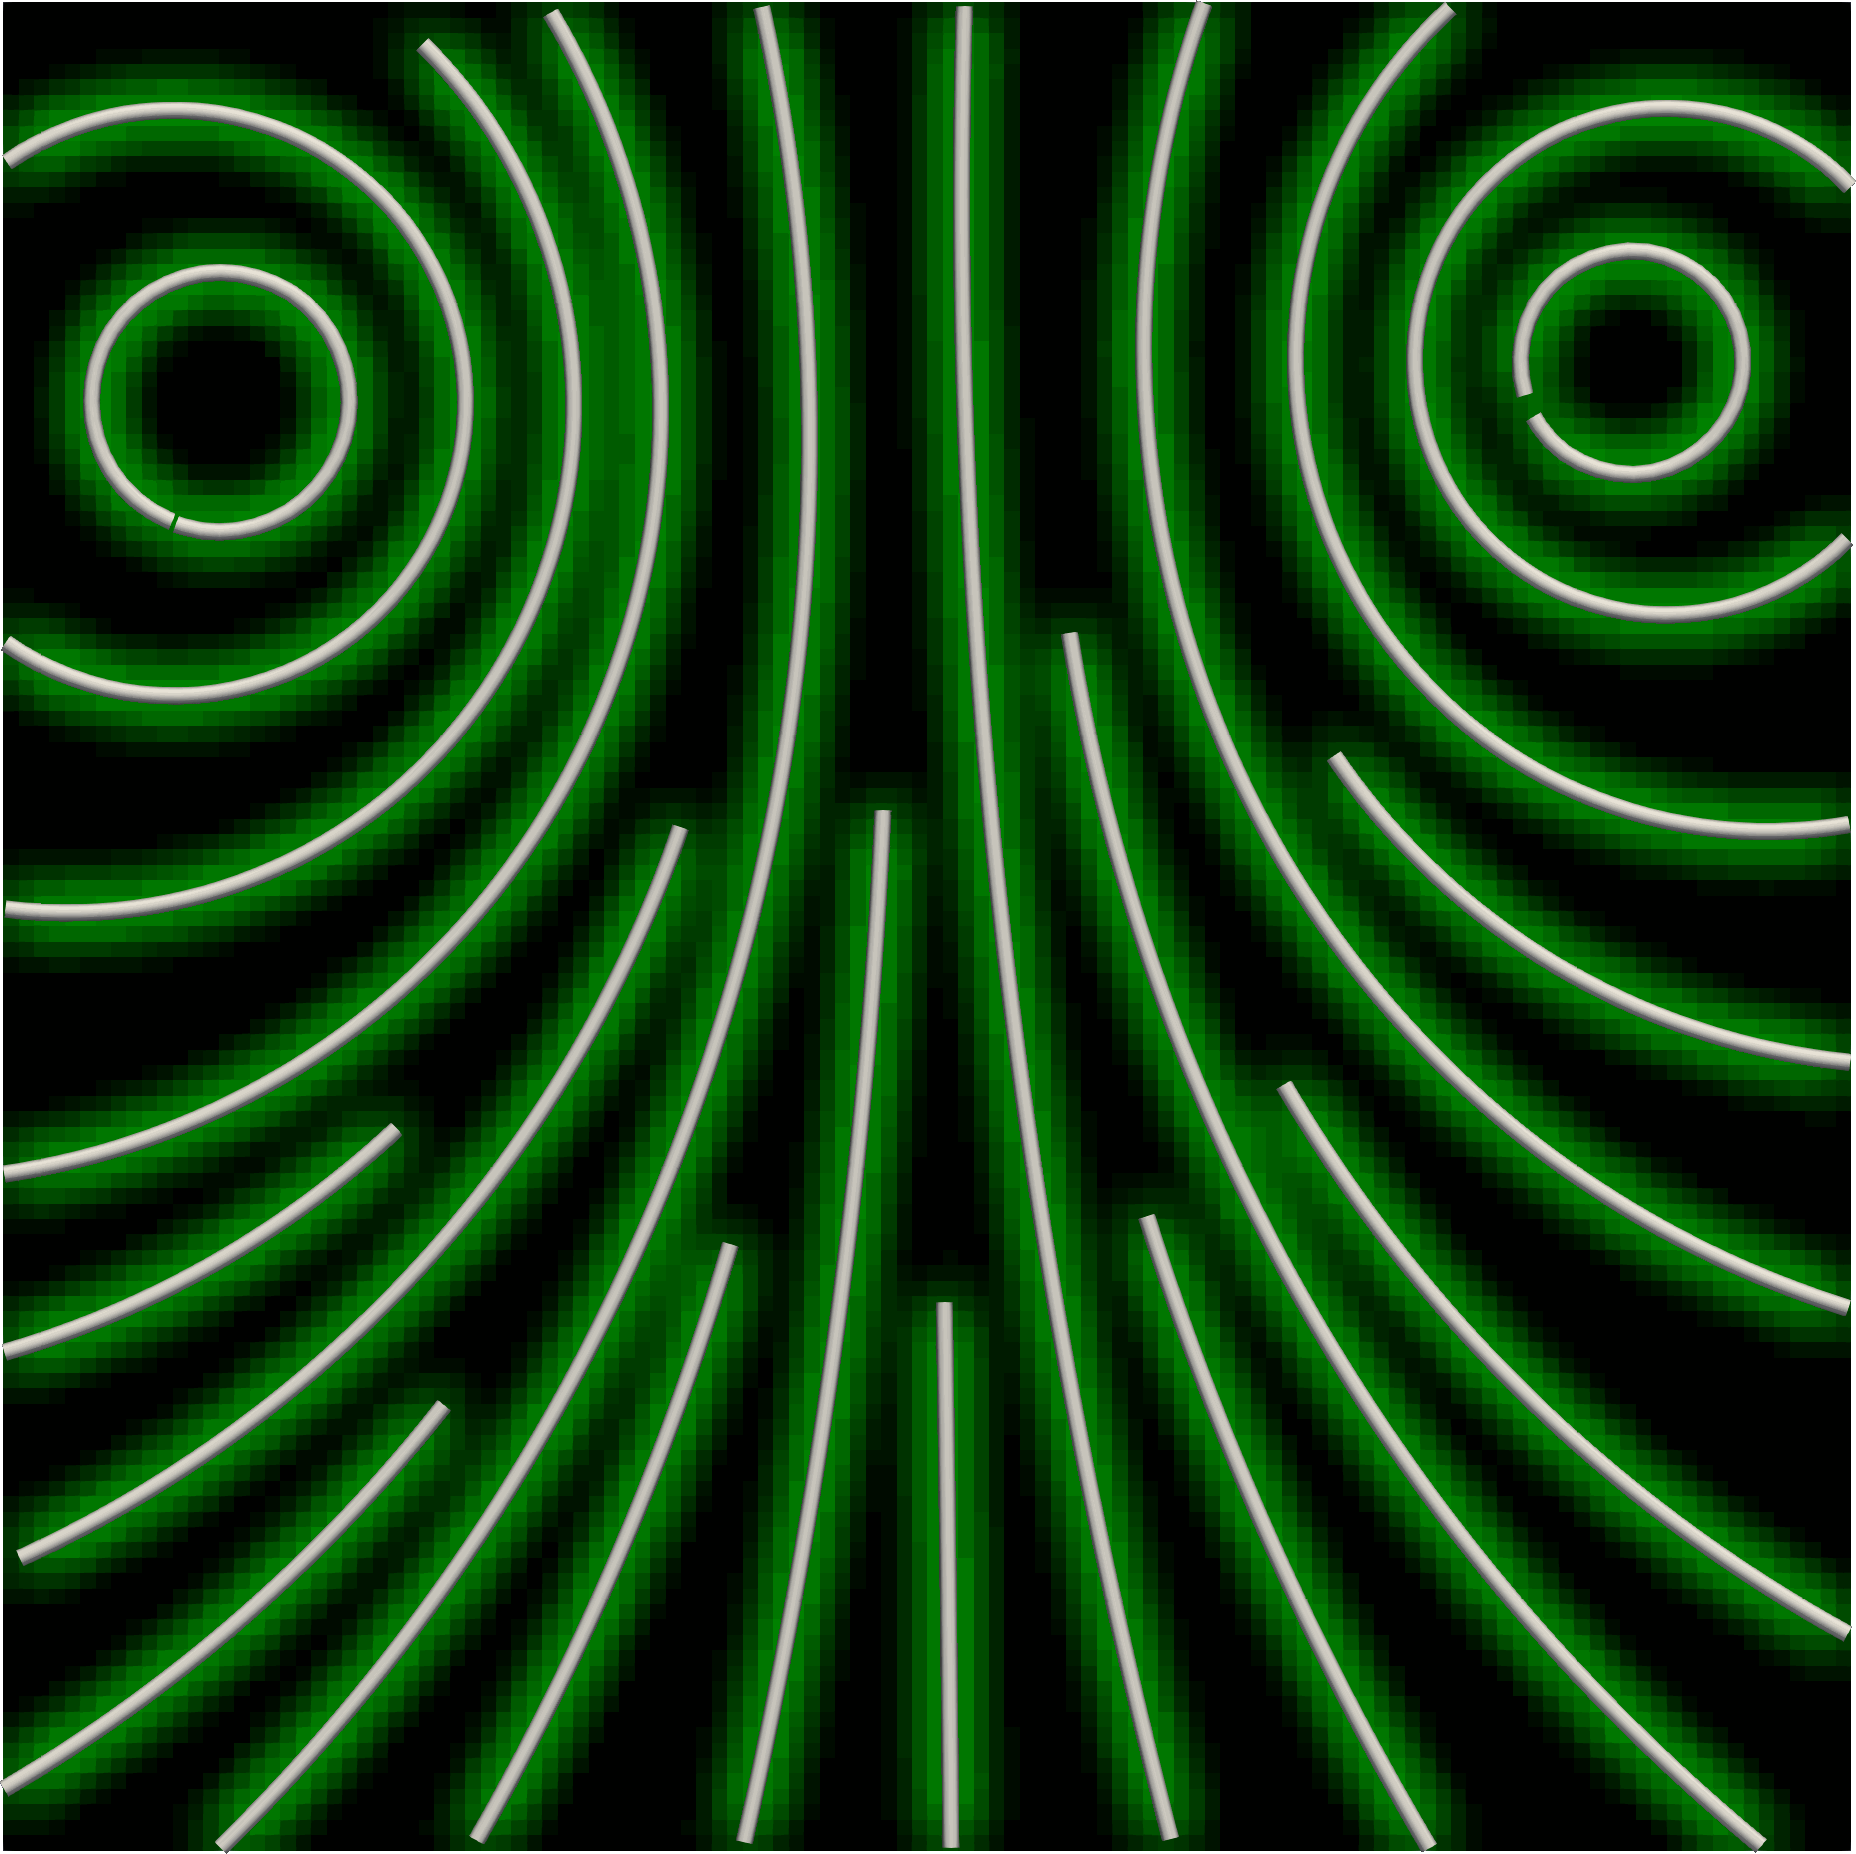
\includegraphics[scale=.055]{figures/AlphaStudy/Gyro23C.0001.png}
        \end{subfigure}
        \begin{subfigure}{.19\textwidth}
            \centering
            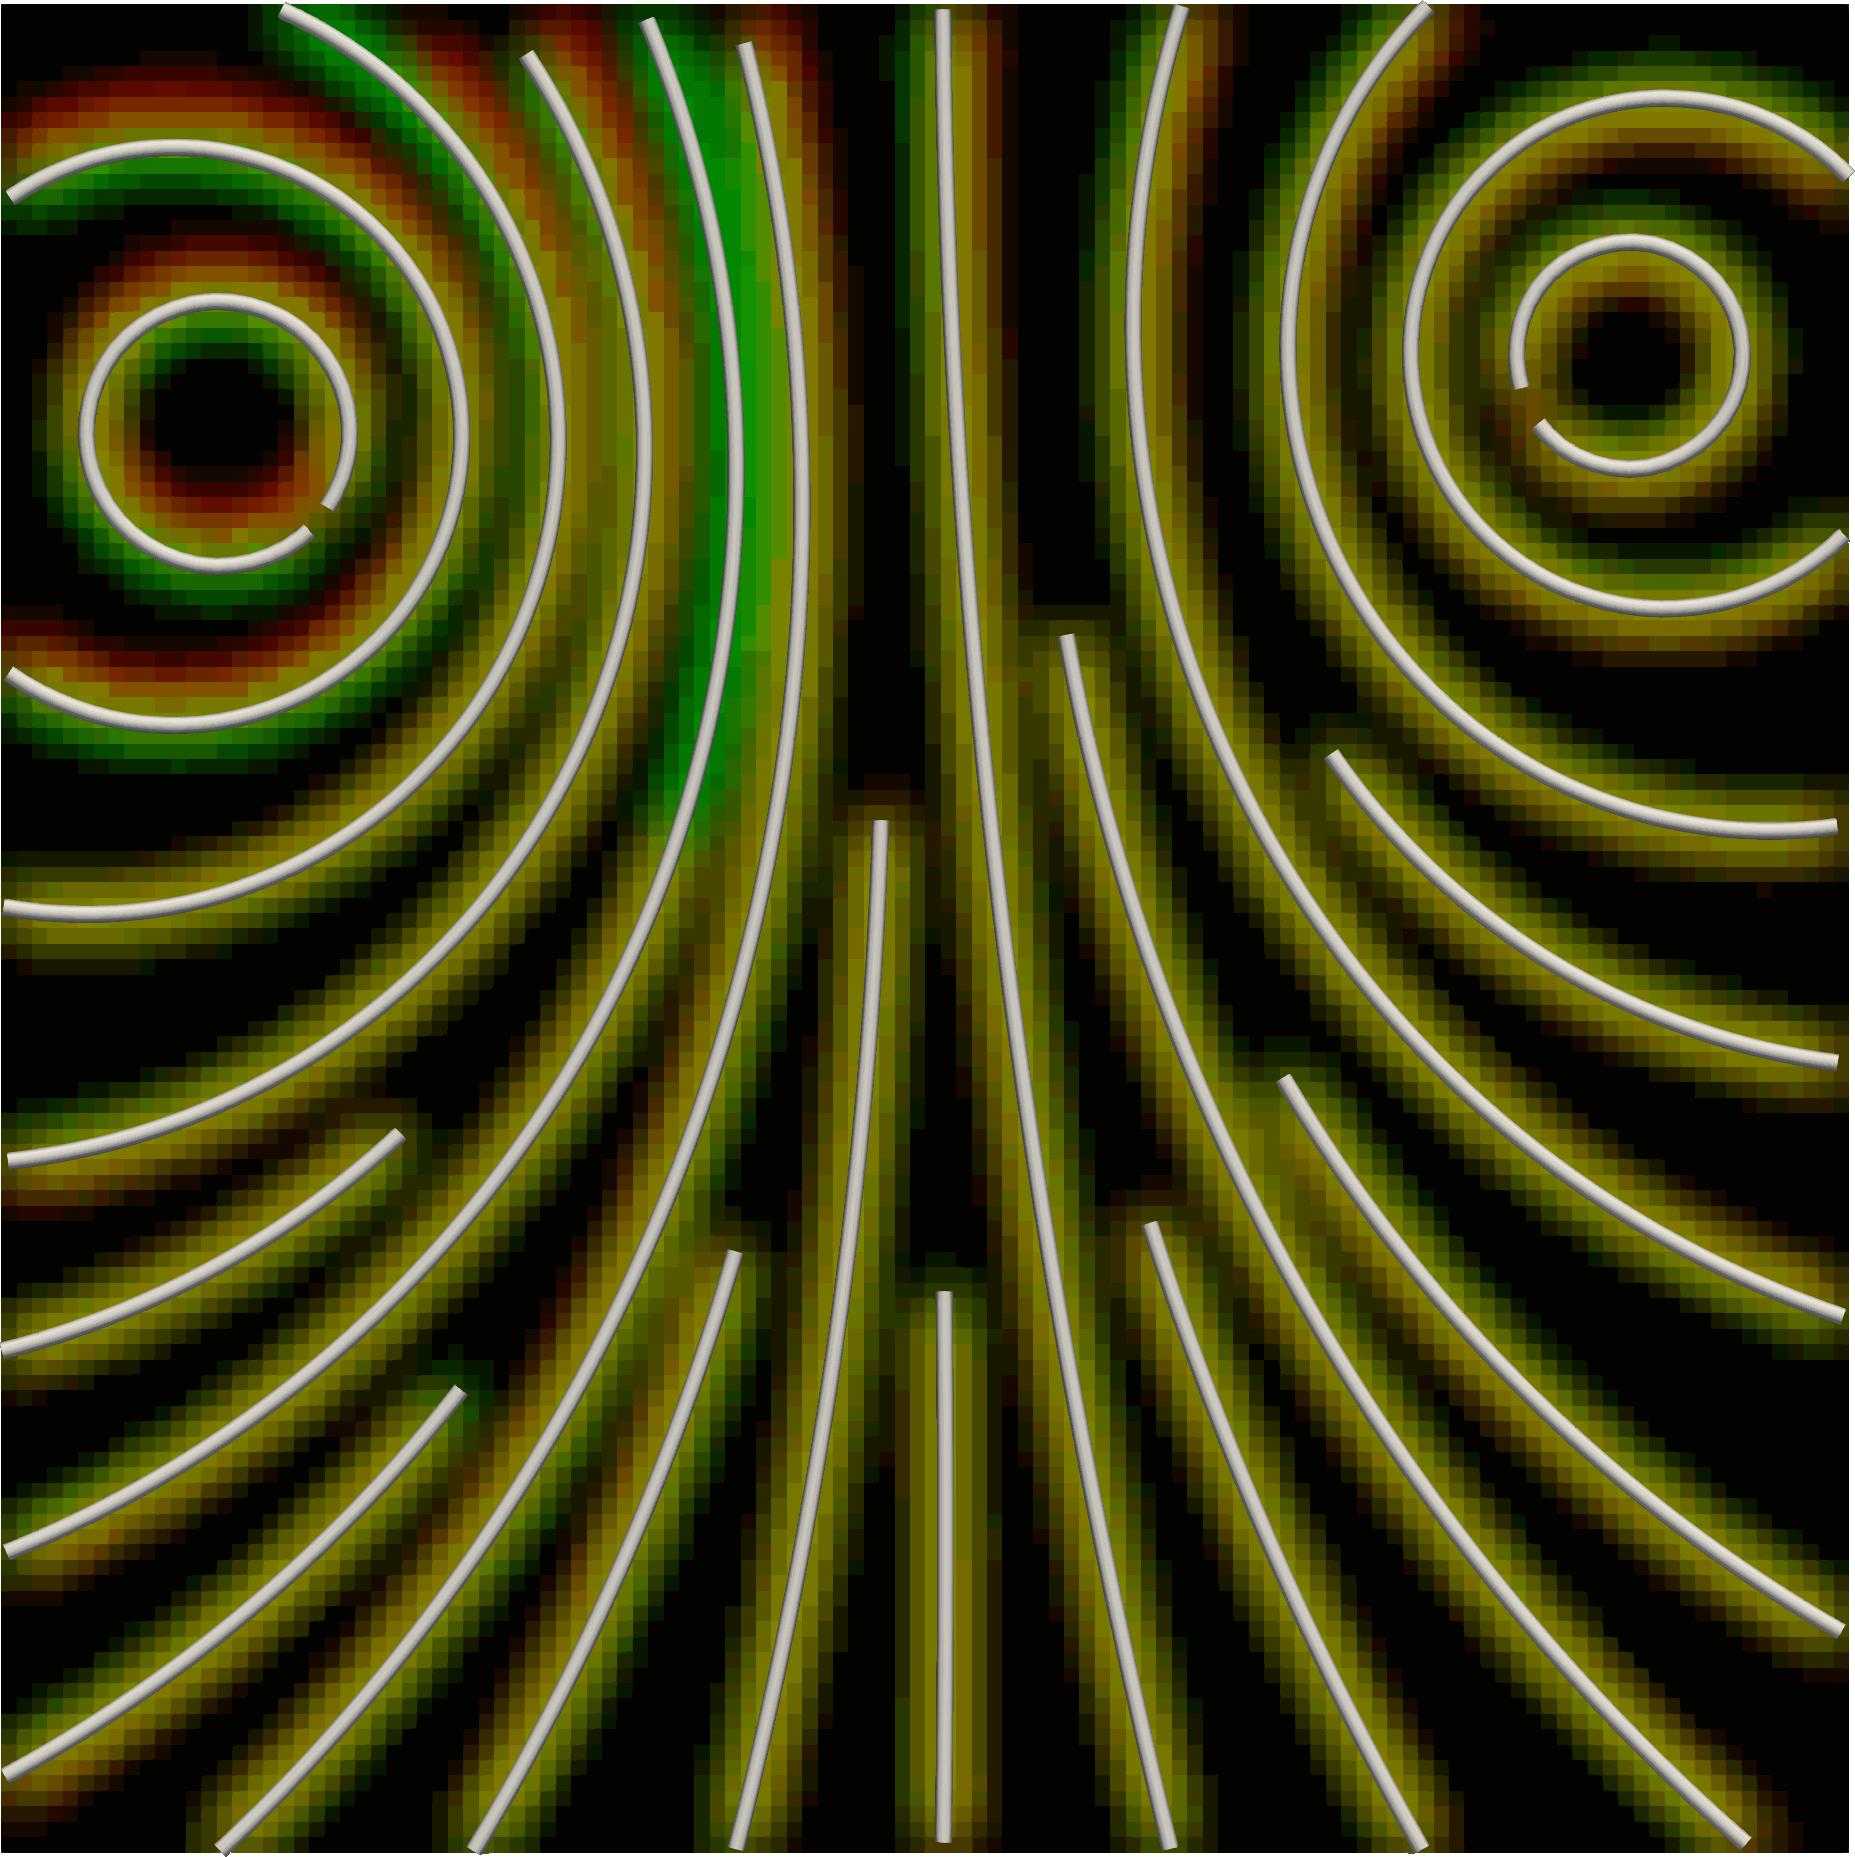
\includegraphics[scale=.055]{figures/AlphaStudy/Gyro23C.0002.png}
        \end{subfigure}
        \begin{subfigure}{.19\textwidth}
            \centering
            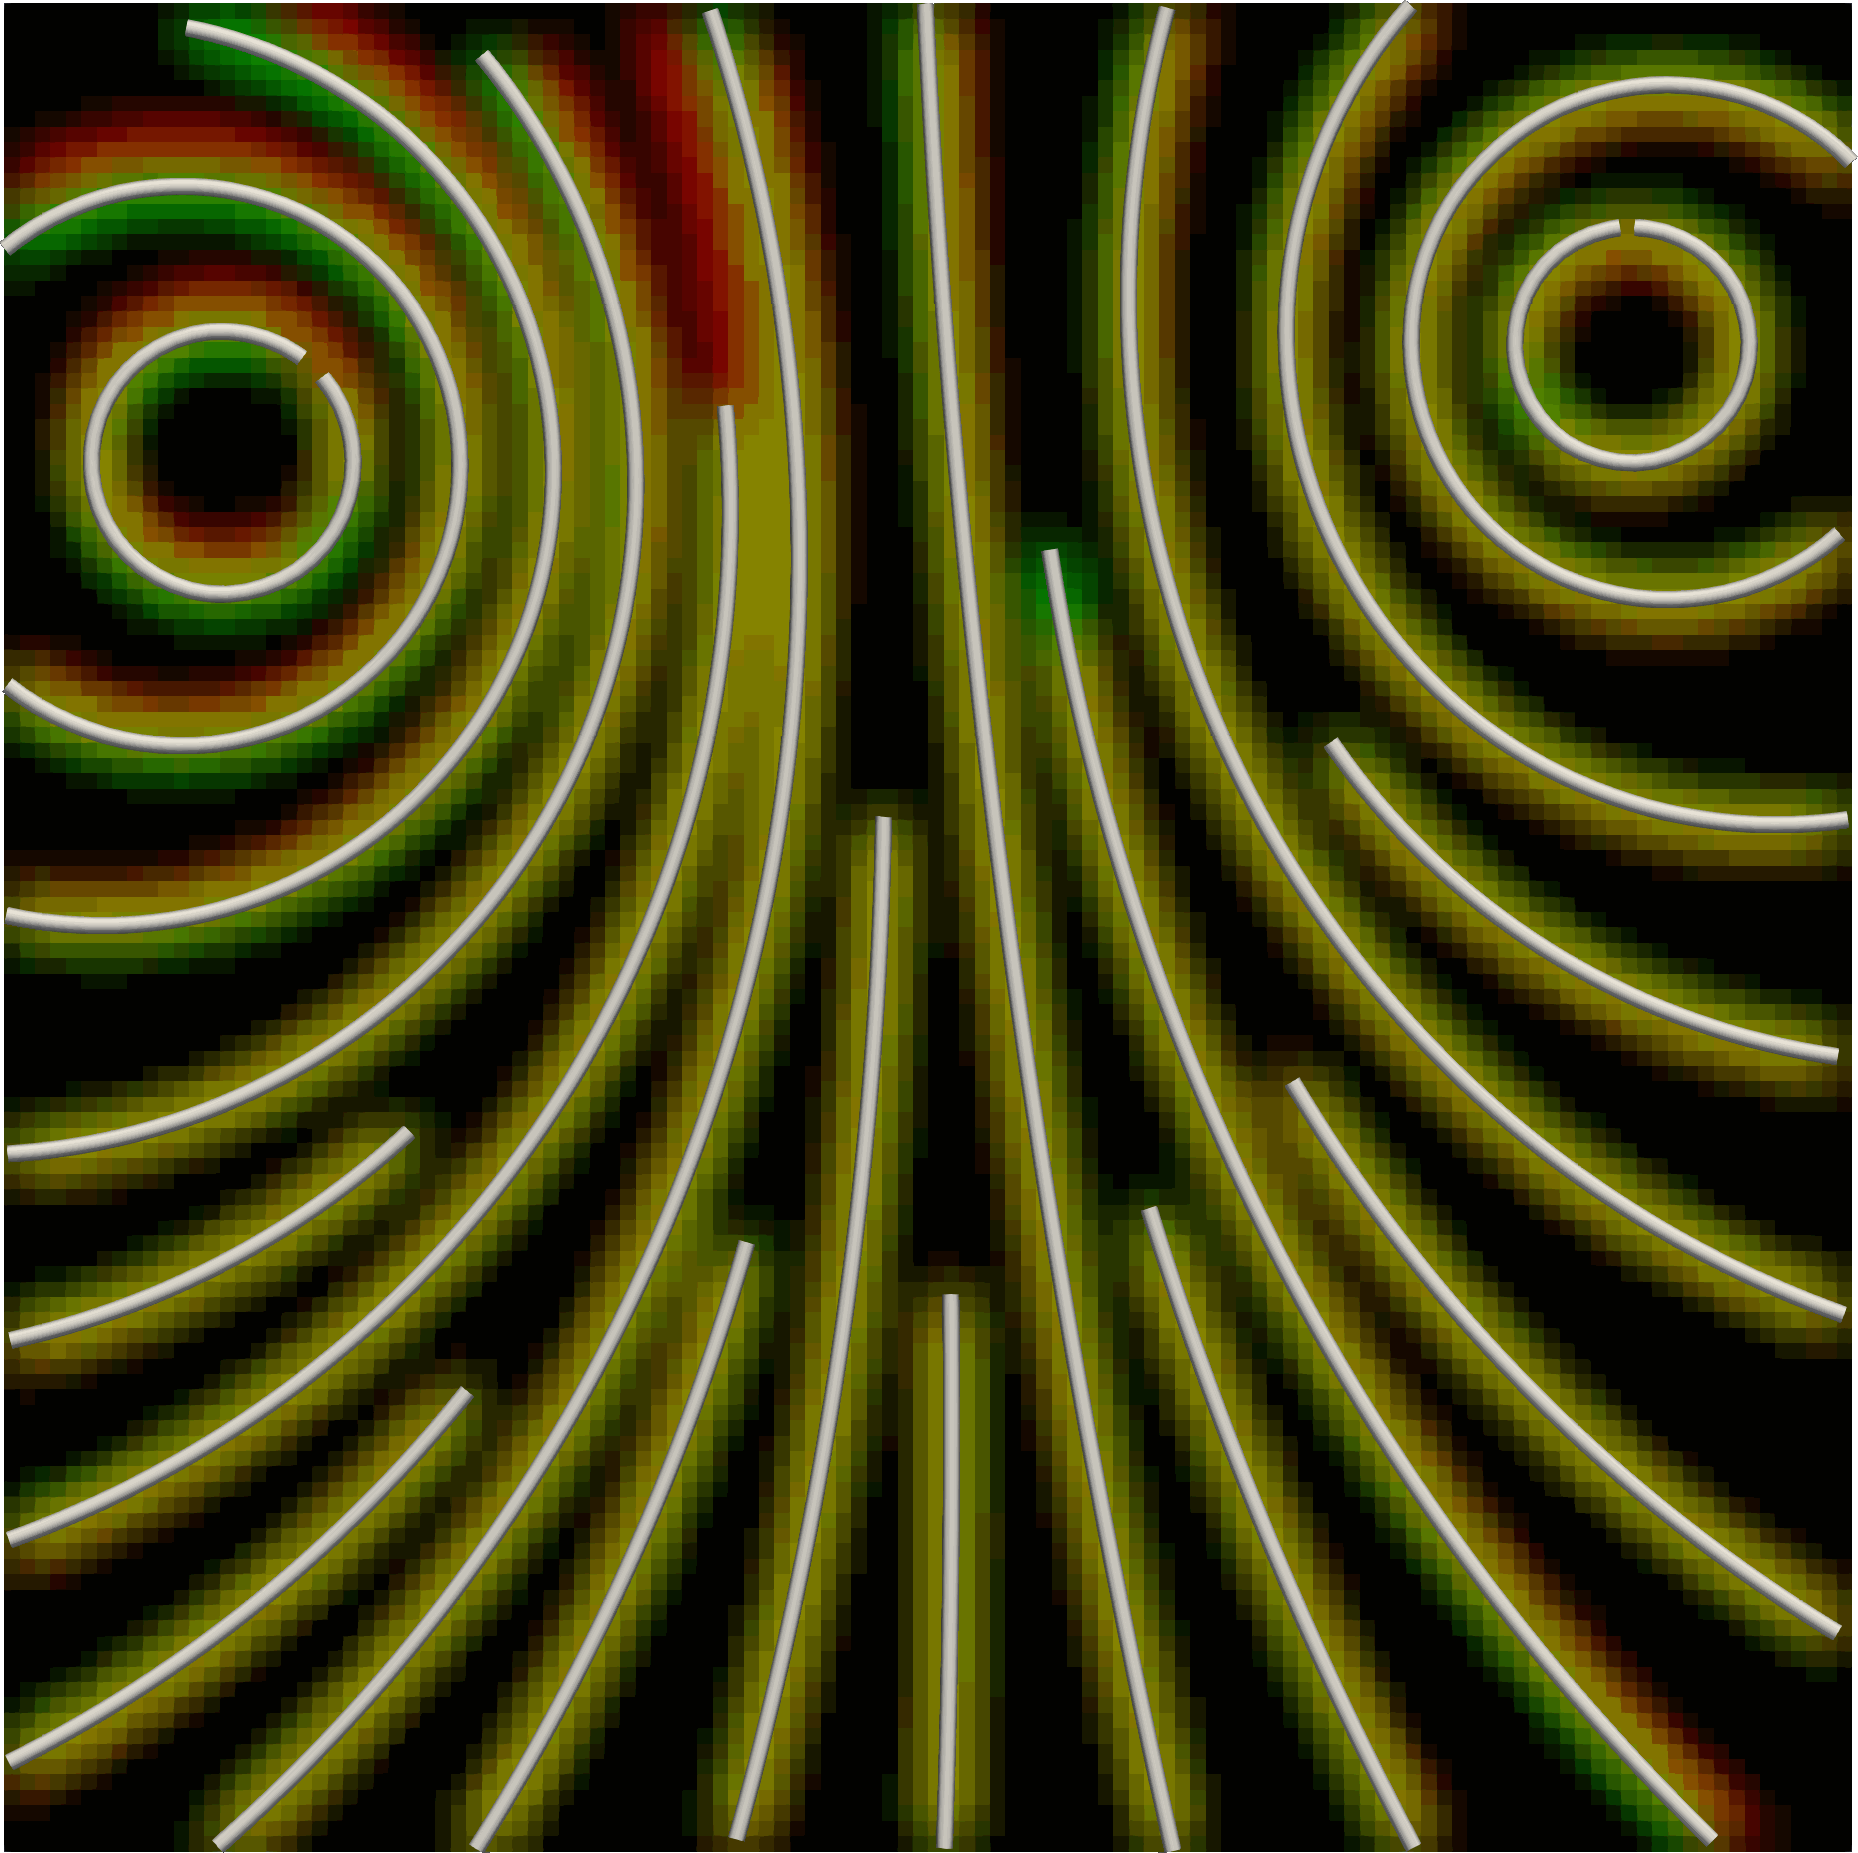
\includegraphics[scale=.055]{figures/AlphaStudy/Gyro23C.0003.png}
        \end{subfigure}
        \begin{subfigure}{.19\textwidth}
            \centering
            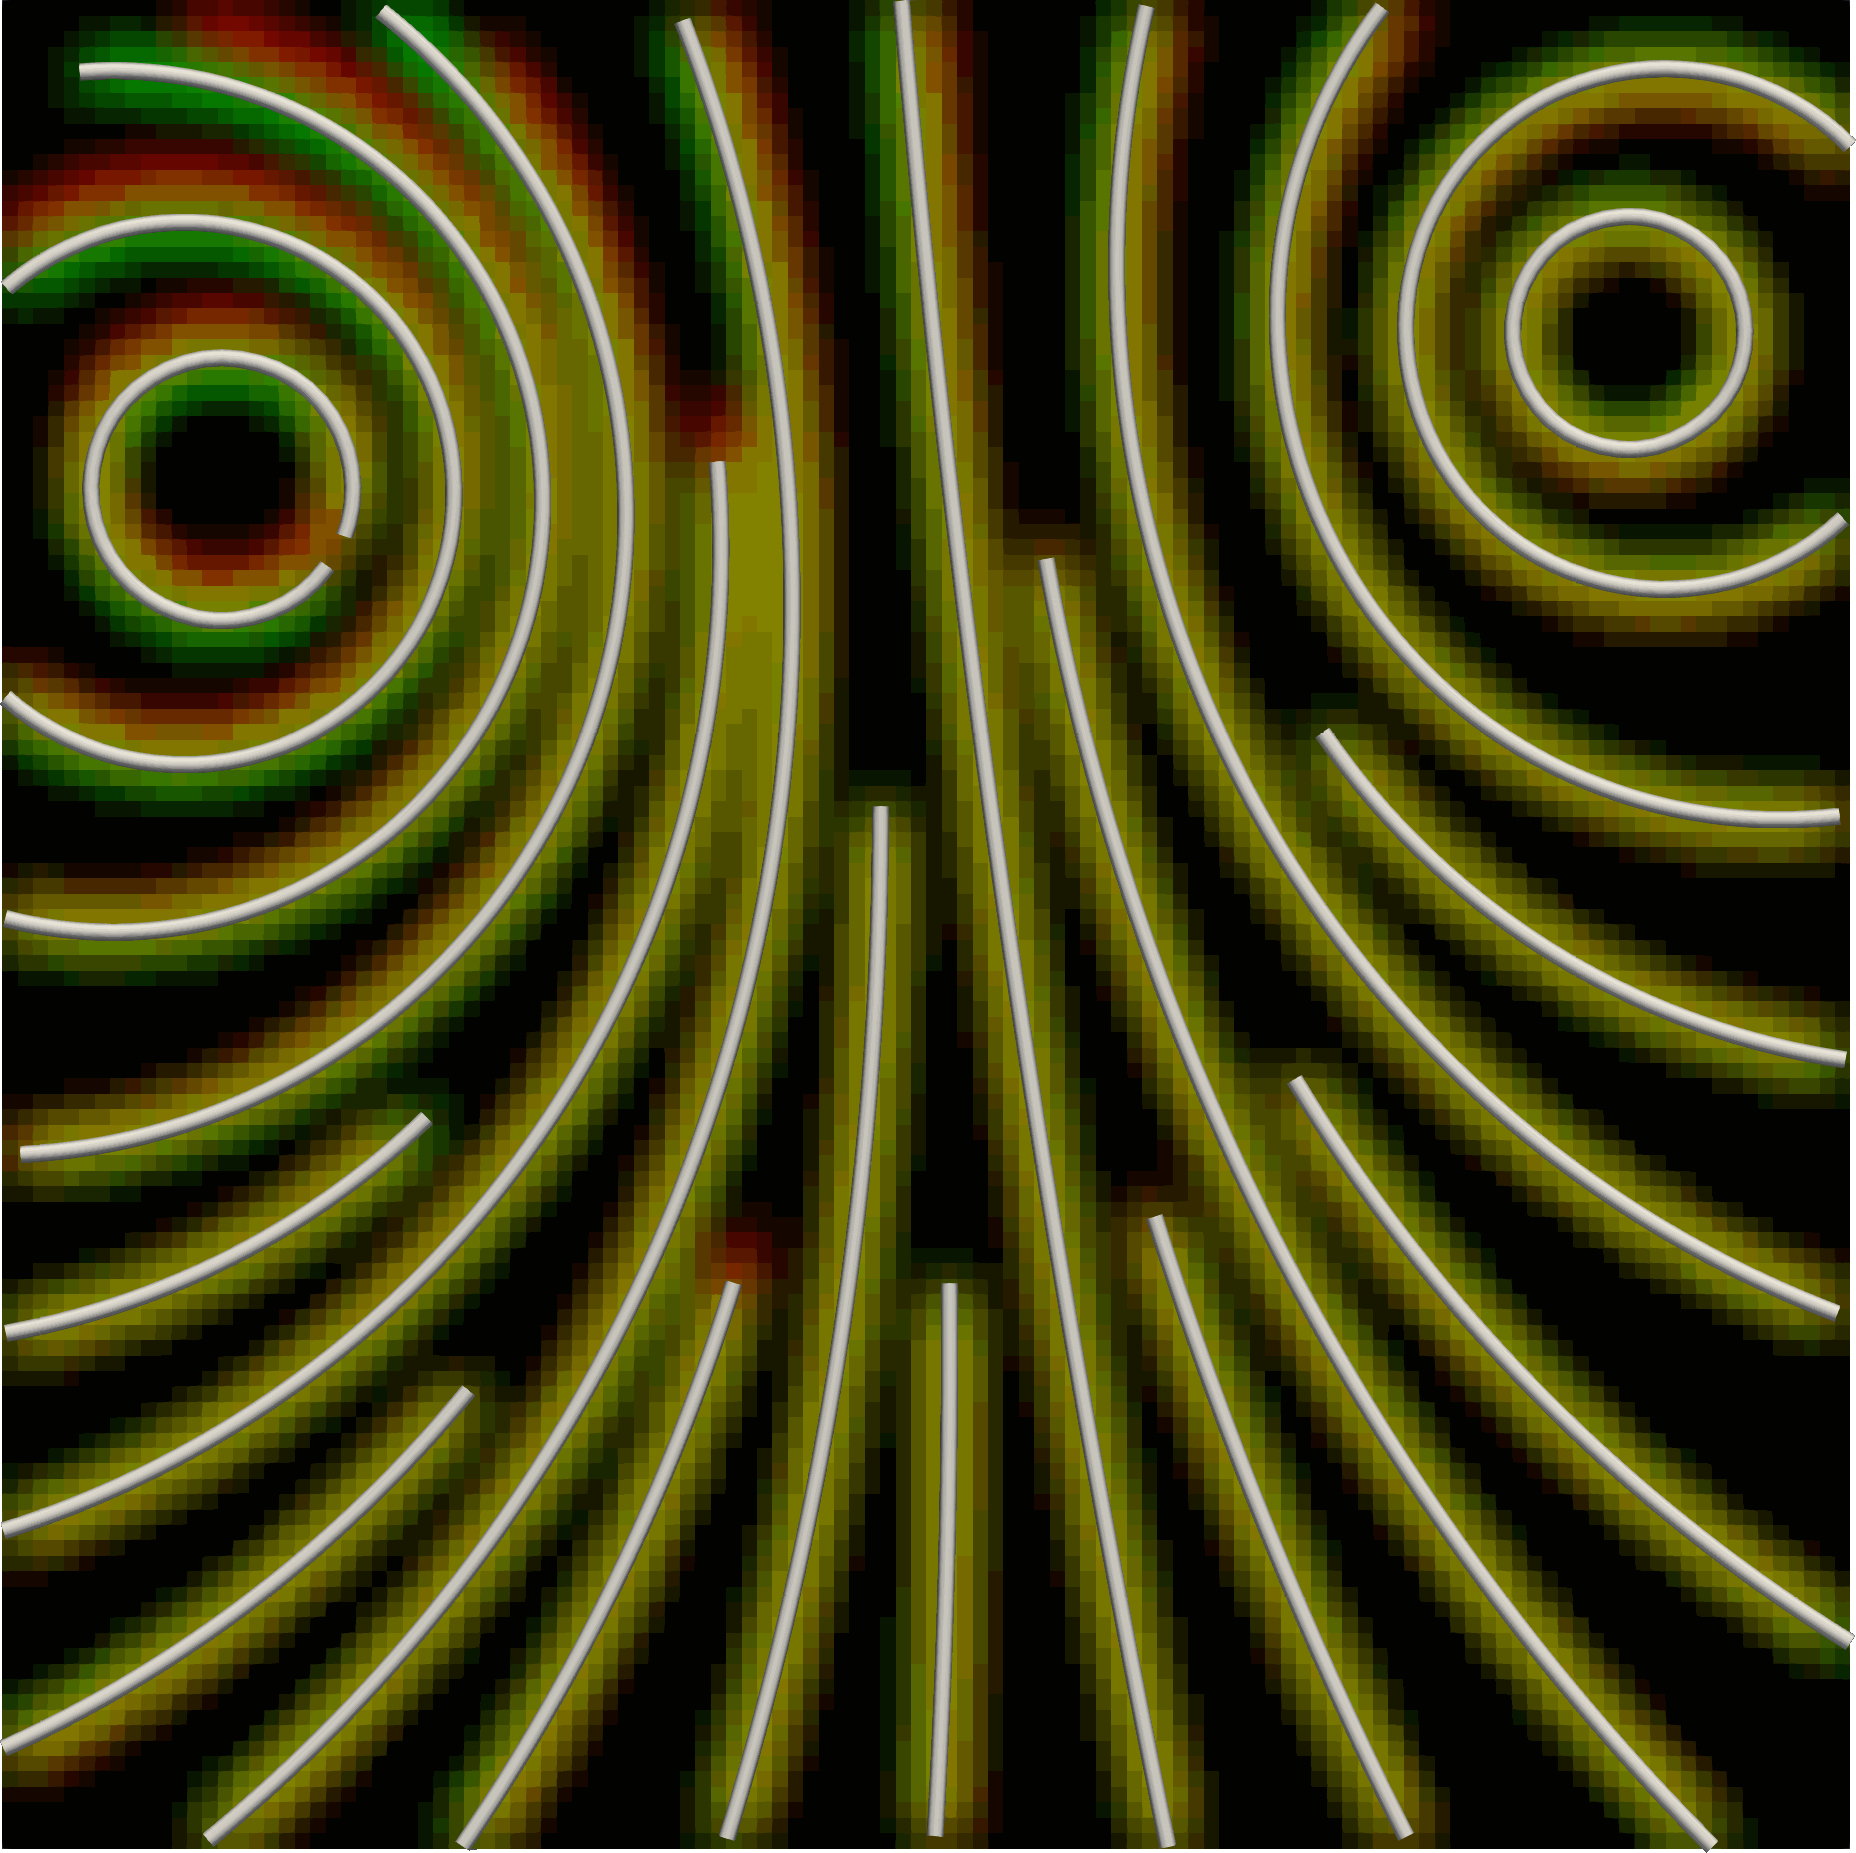
\includegraphics[scale=.055]{figures/AlphaStudy/Gyro23C.0004.png}
        \end{subfigure}
        \caption*{(c)}
    \end{subfigure}
    % 5 x 3 / 3 coherence
    \begin{subfigure}{\textwidth}
        \begin{subfigure}{.19\textwidth}
            \centering
            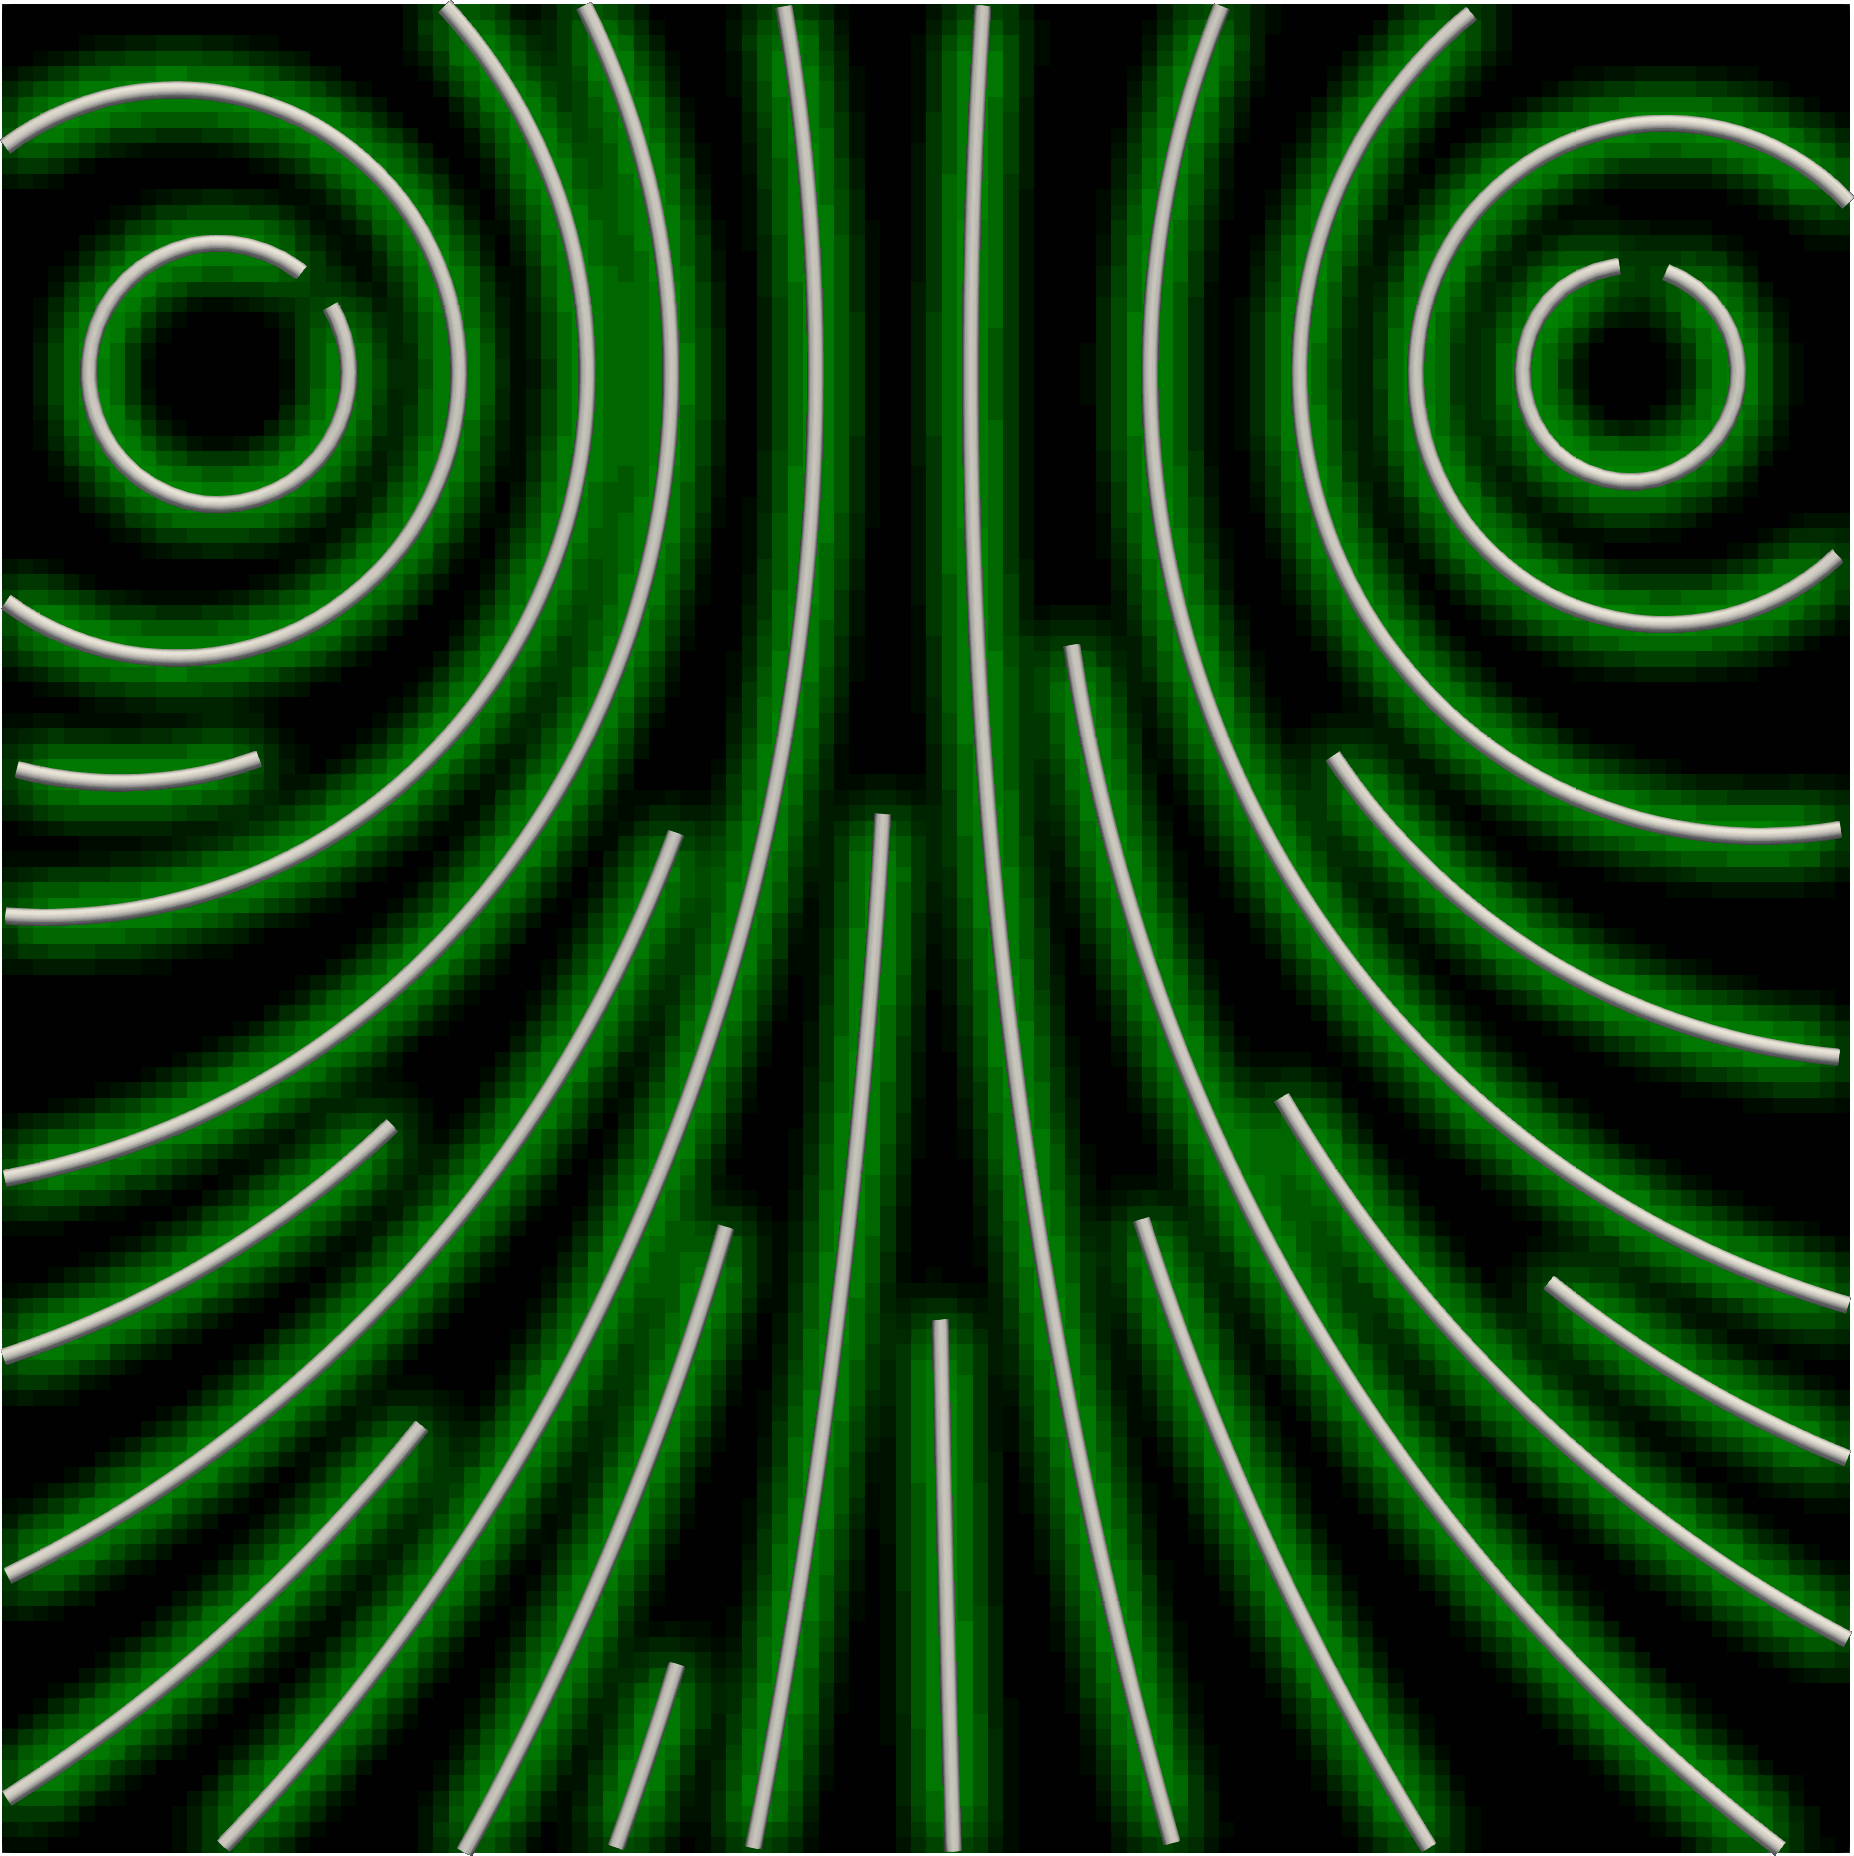
\includegraphics[scale=.055]{figures/AlphaStudy/Gyro33C.0000.png}
        \end{subfigure}
        \begin{subfigure}{.19\textwidth}
            \centering
            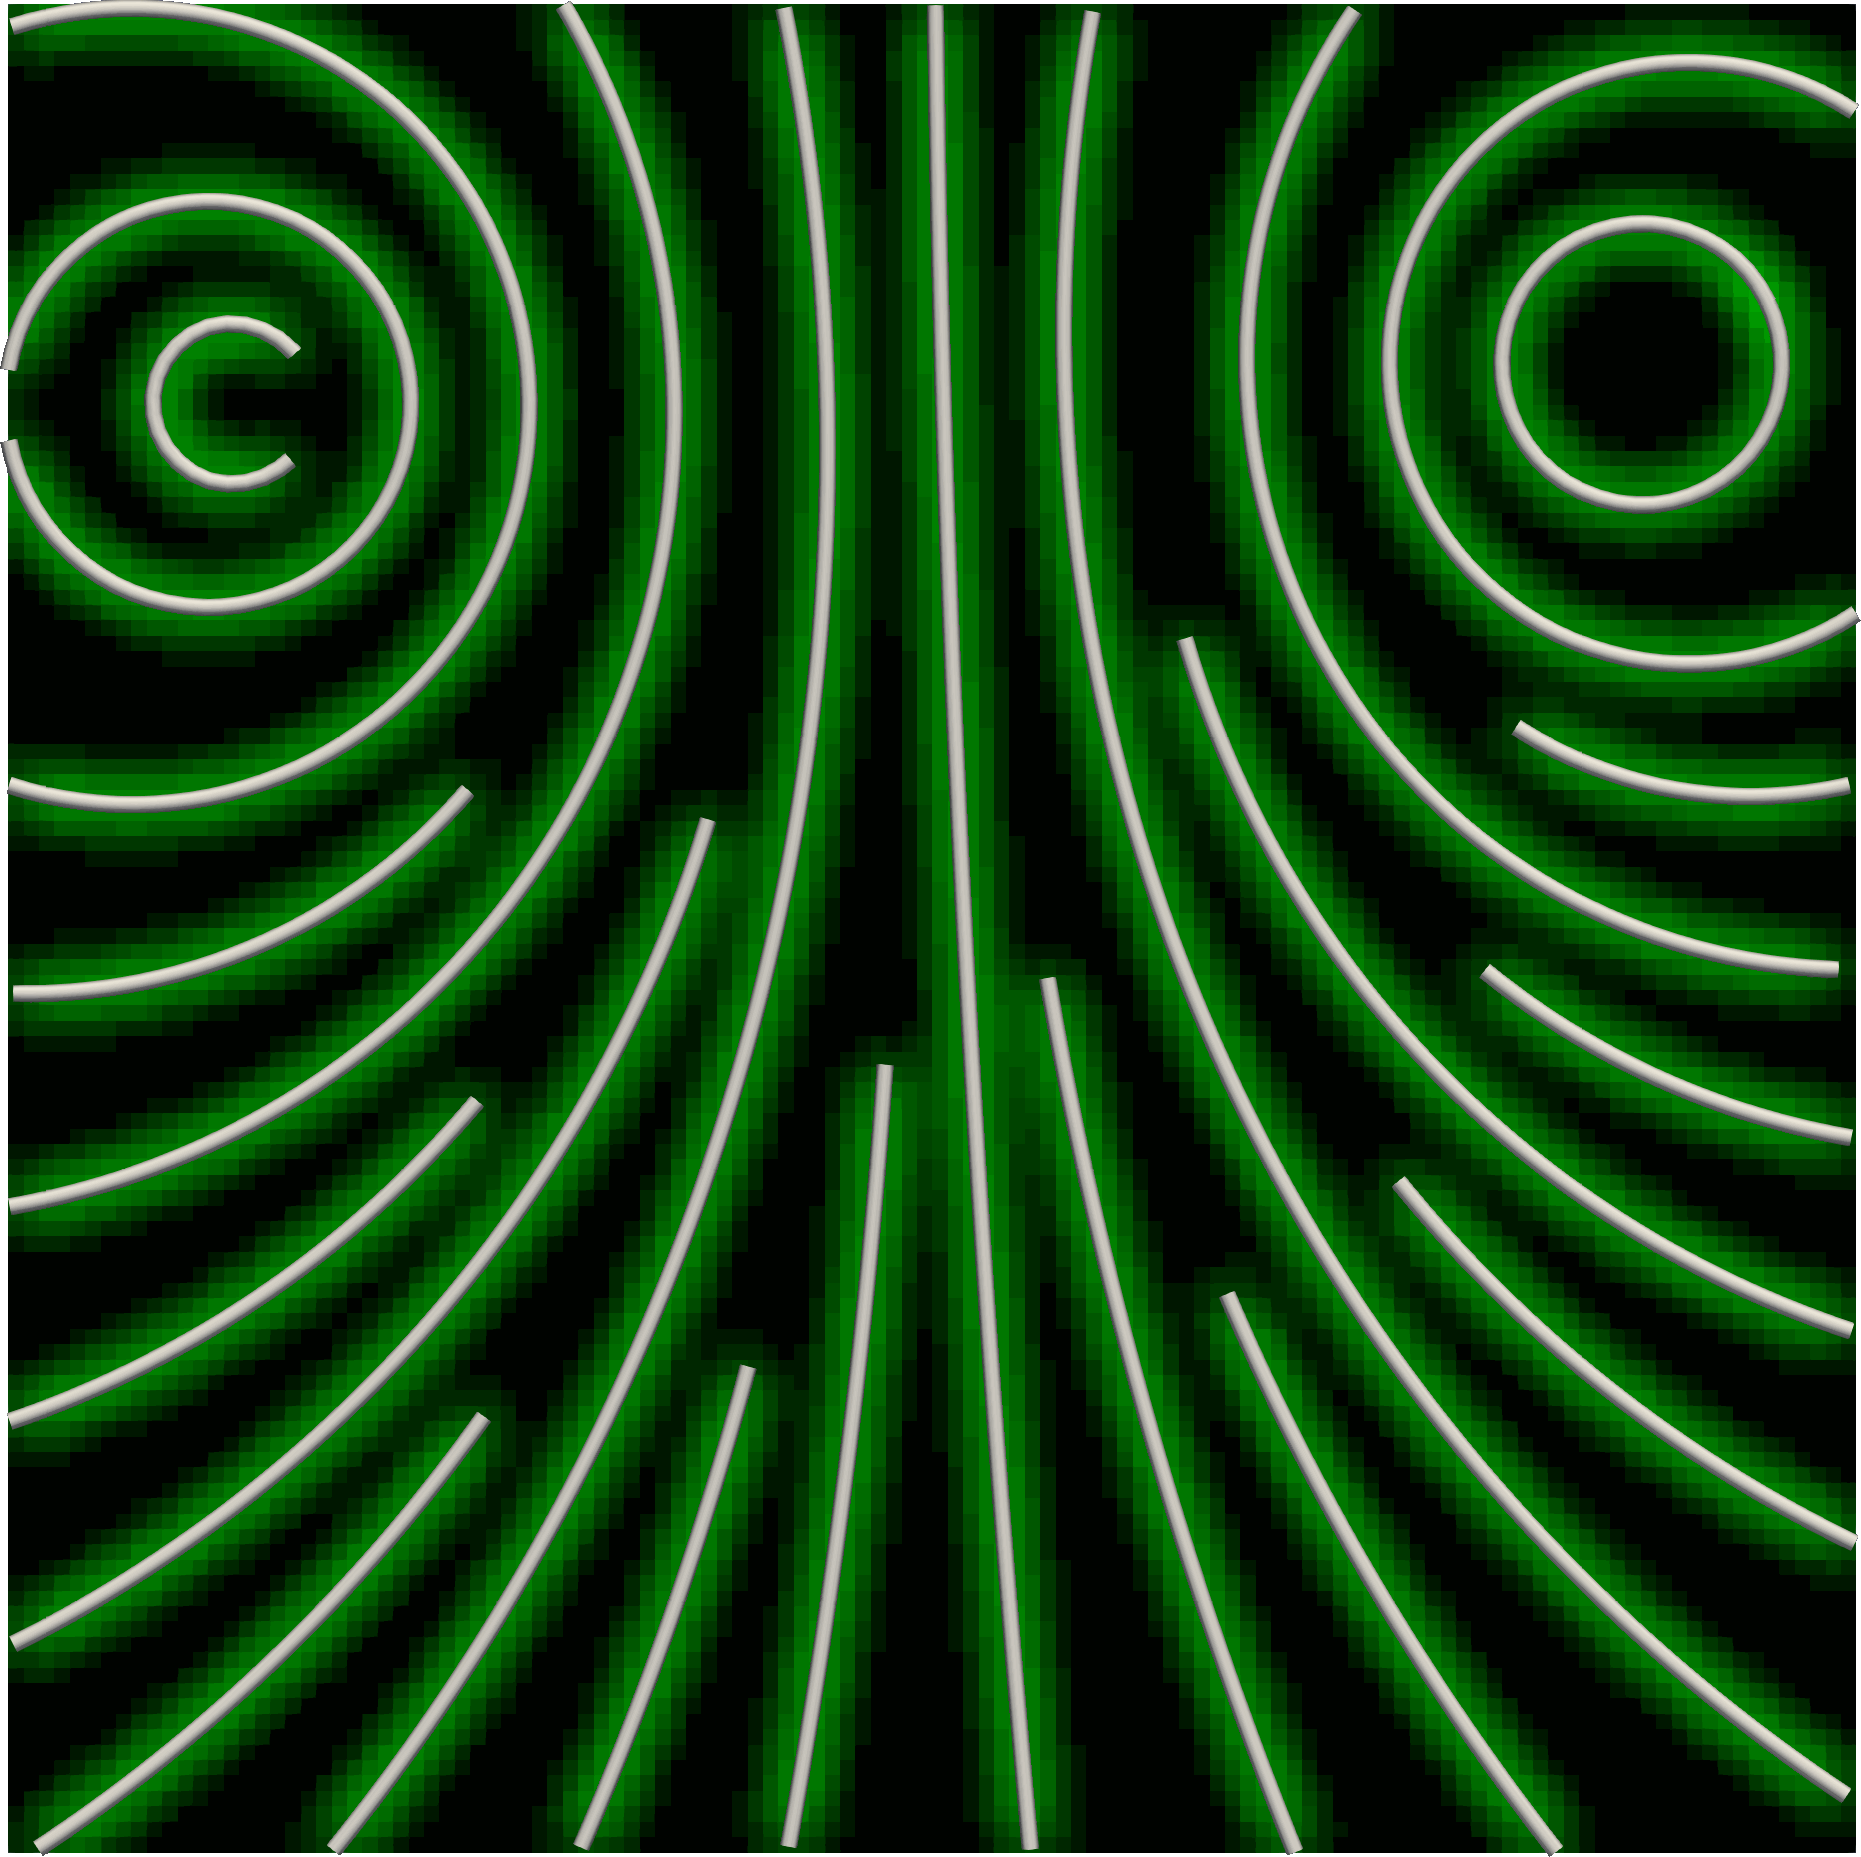
\includegraphics[scale=.055]{figures/AlphaStudy/Gyro33C.0001.png}
        \end{subfigure}
        \begin{subfigure}{.19\textwidth}
            \centering
            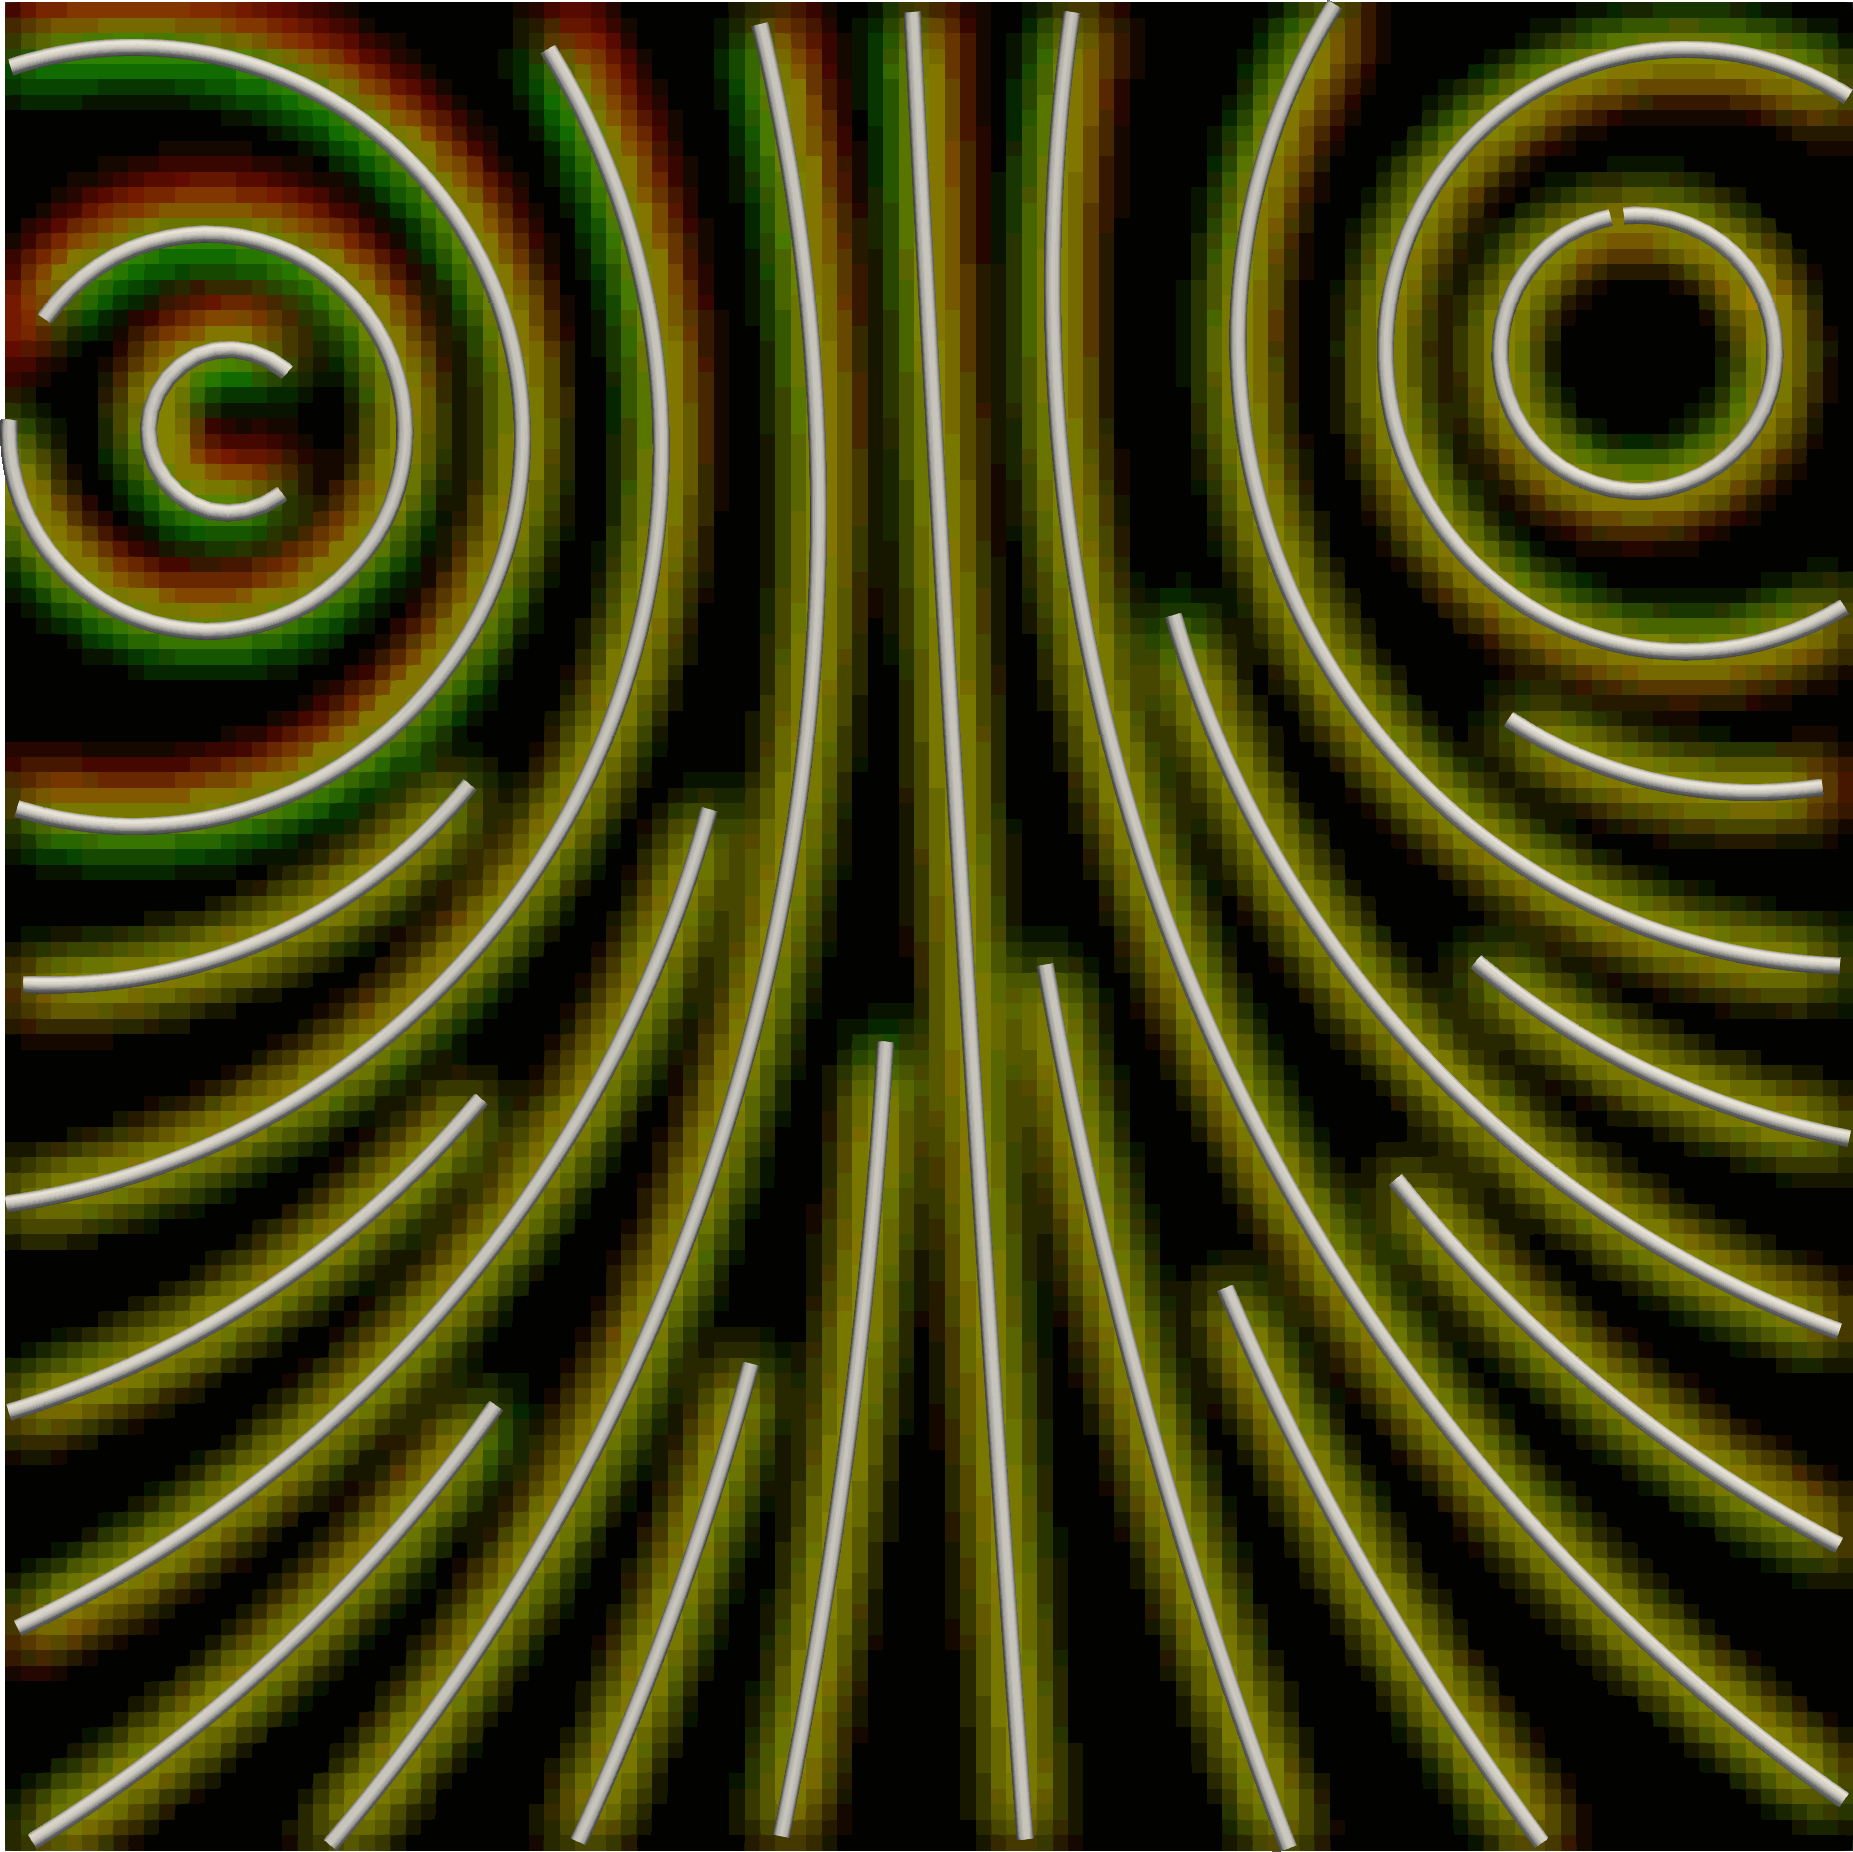
\includegraphics[scale=.055]{figures/AlphaStudy/Gyro33C.0002.png}
        \end{subfigure}
        \begin{subfigure}{.19\textwidth}
            \centering
            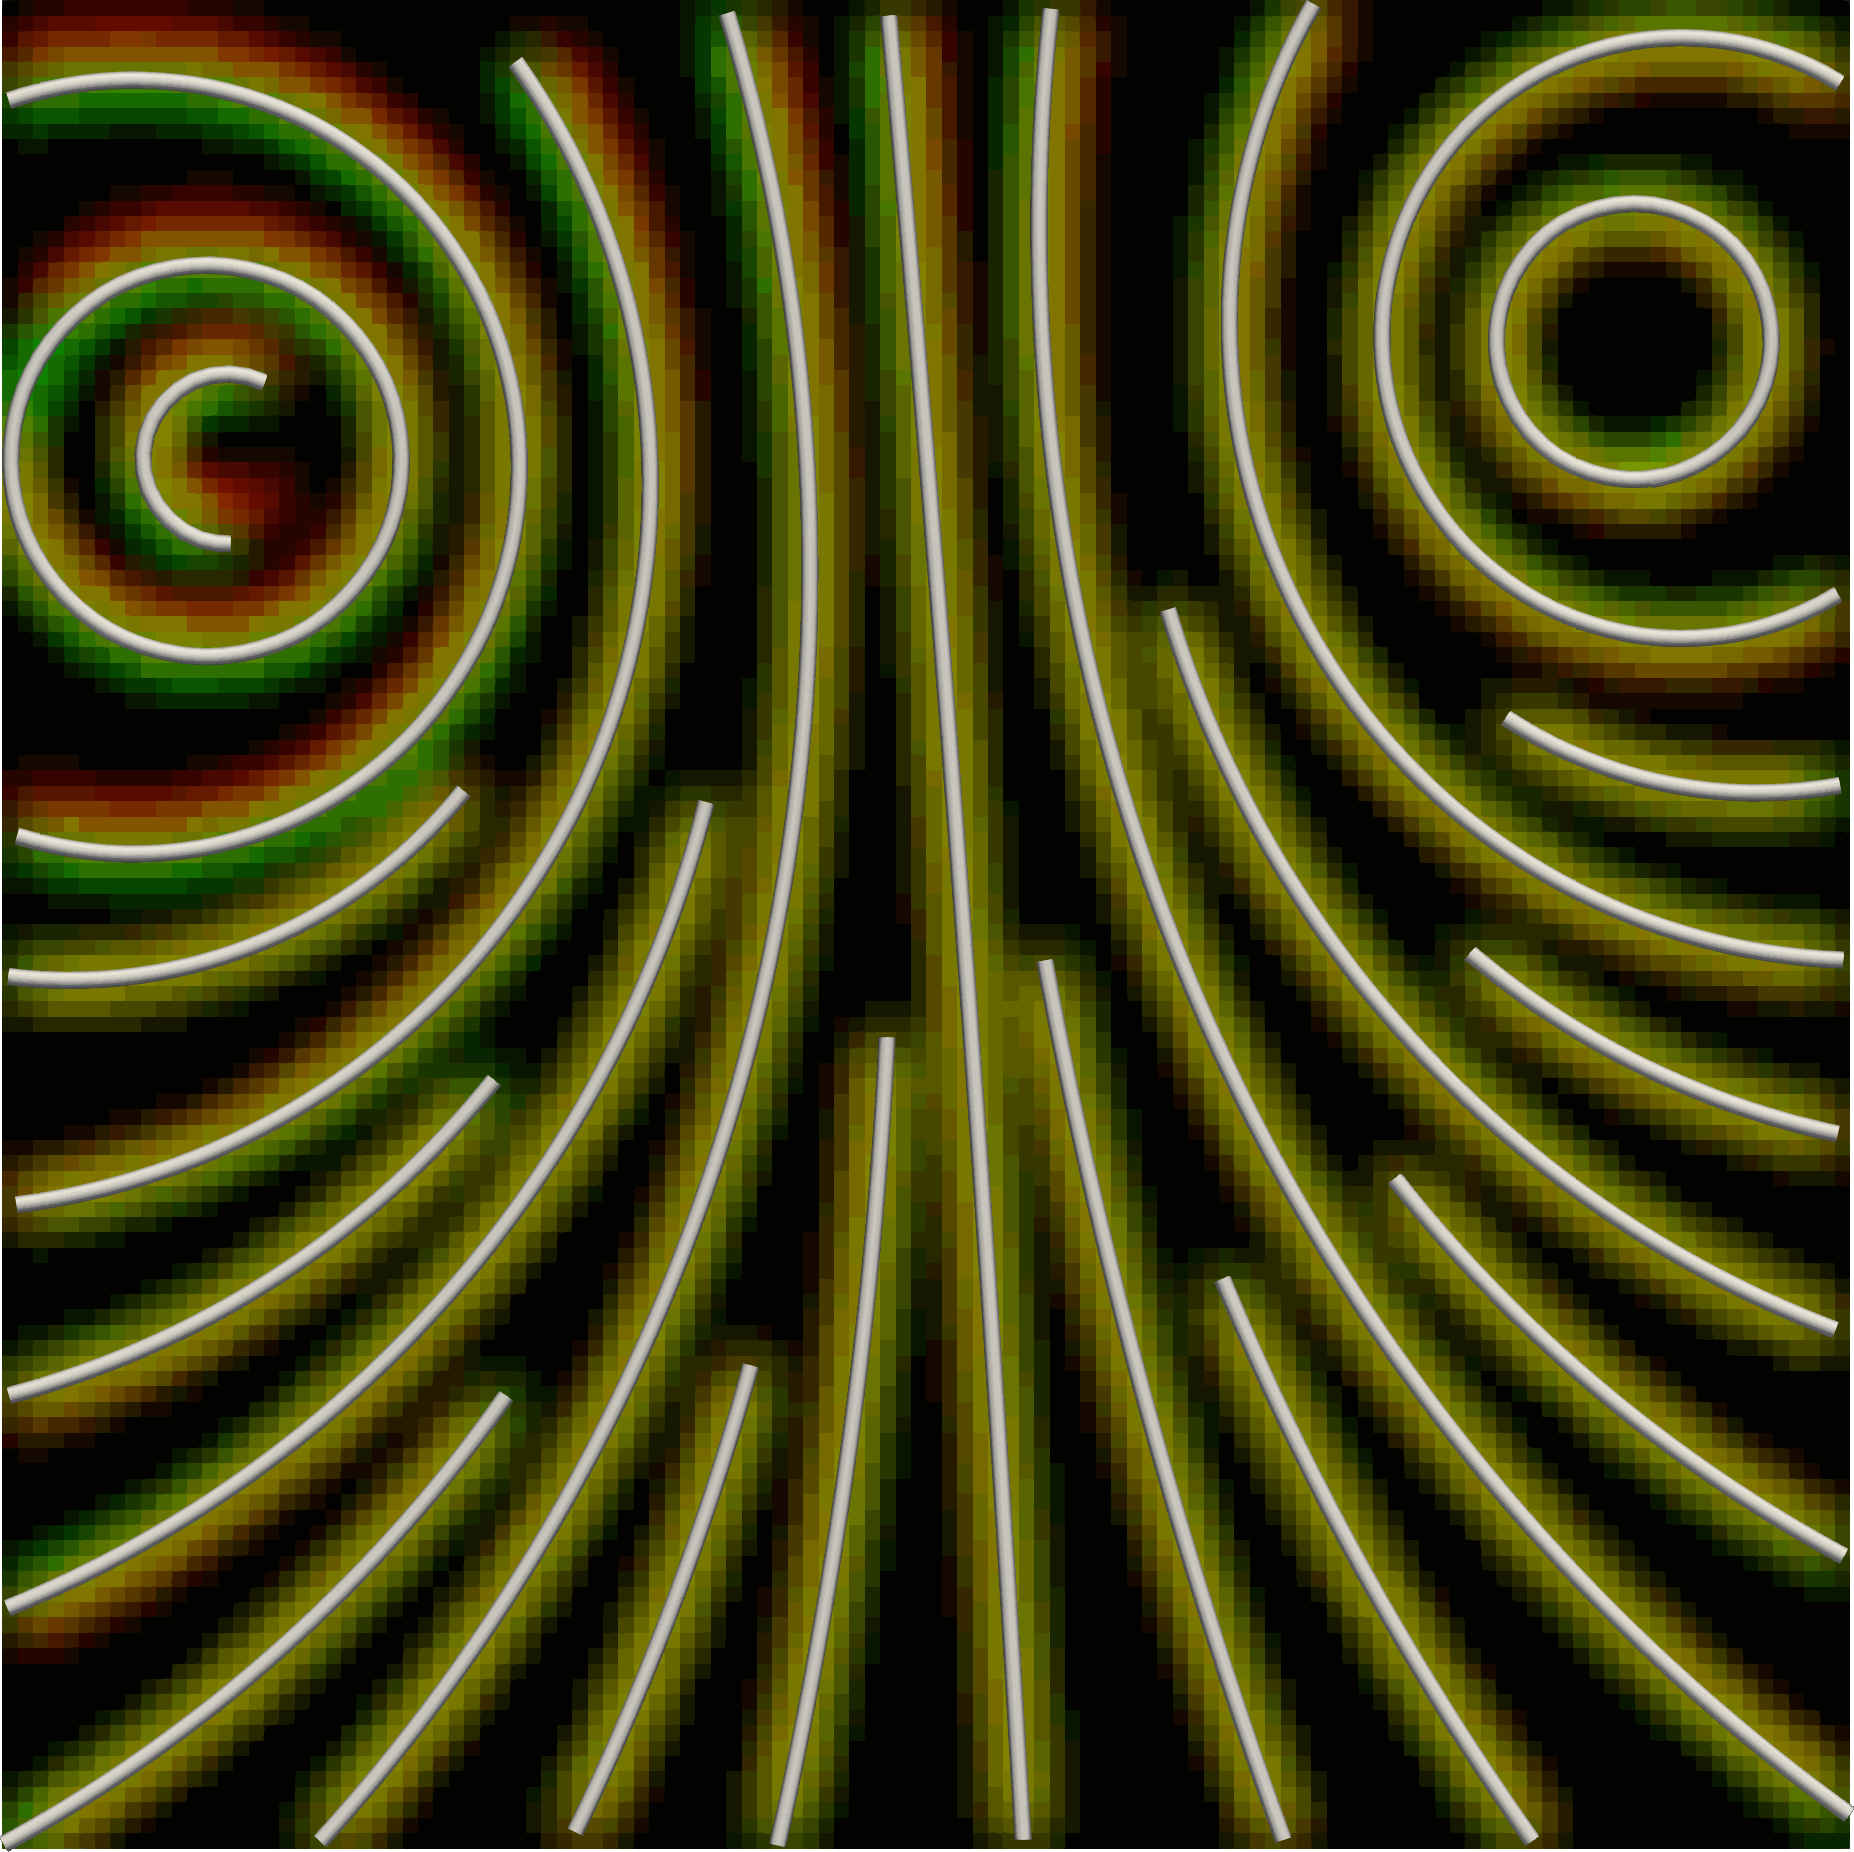
\includegraphics[scale=.055]{figures/AlphaStudy/Gyro33C.0003.png}
        \end{subfigure}
        \begin{subfigure}{.19\textwidth}
            \centering
            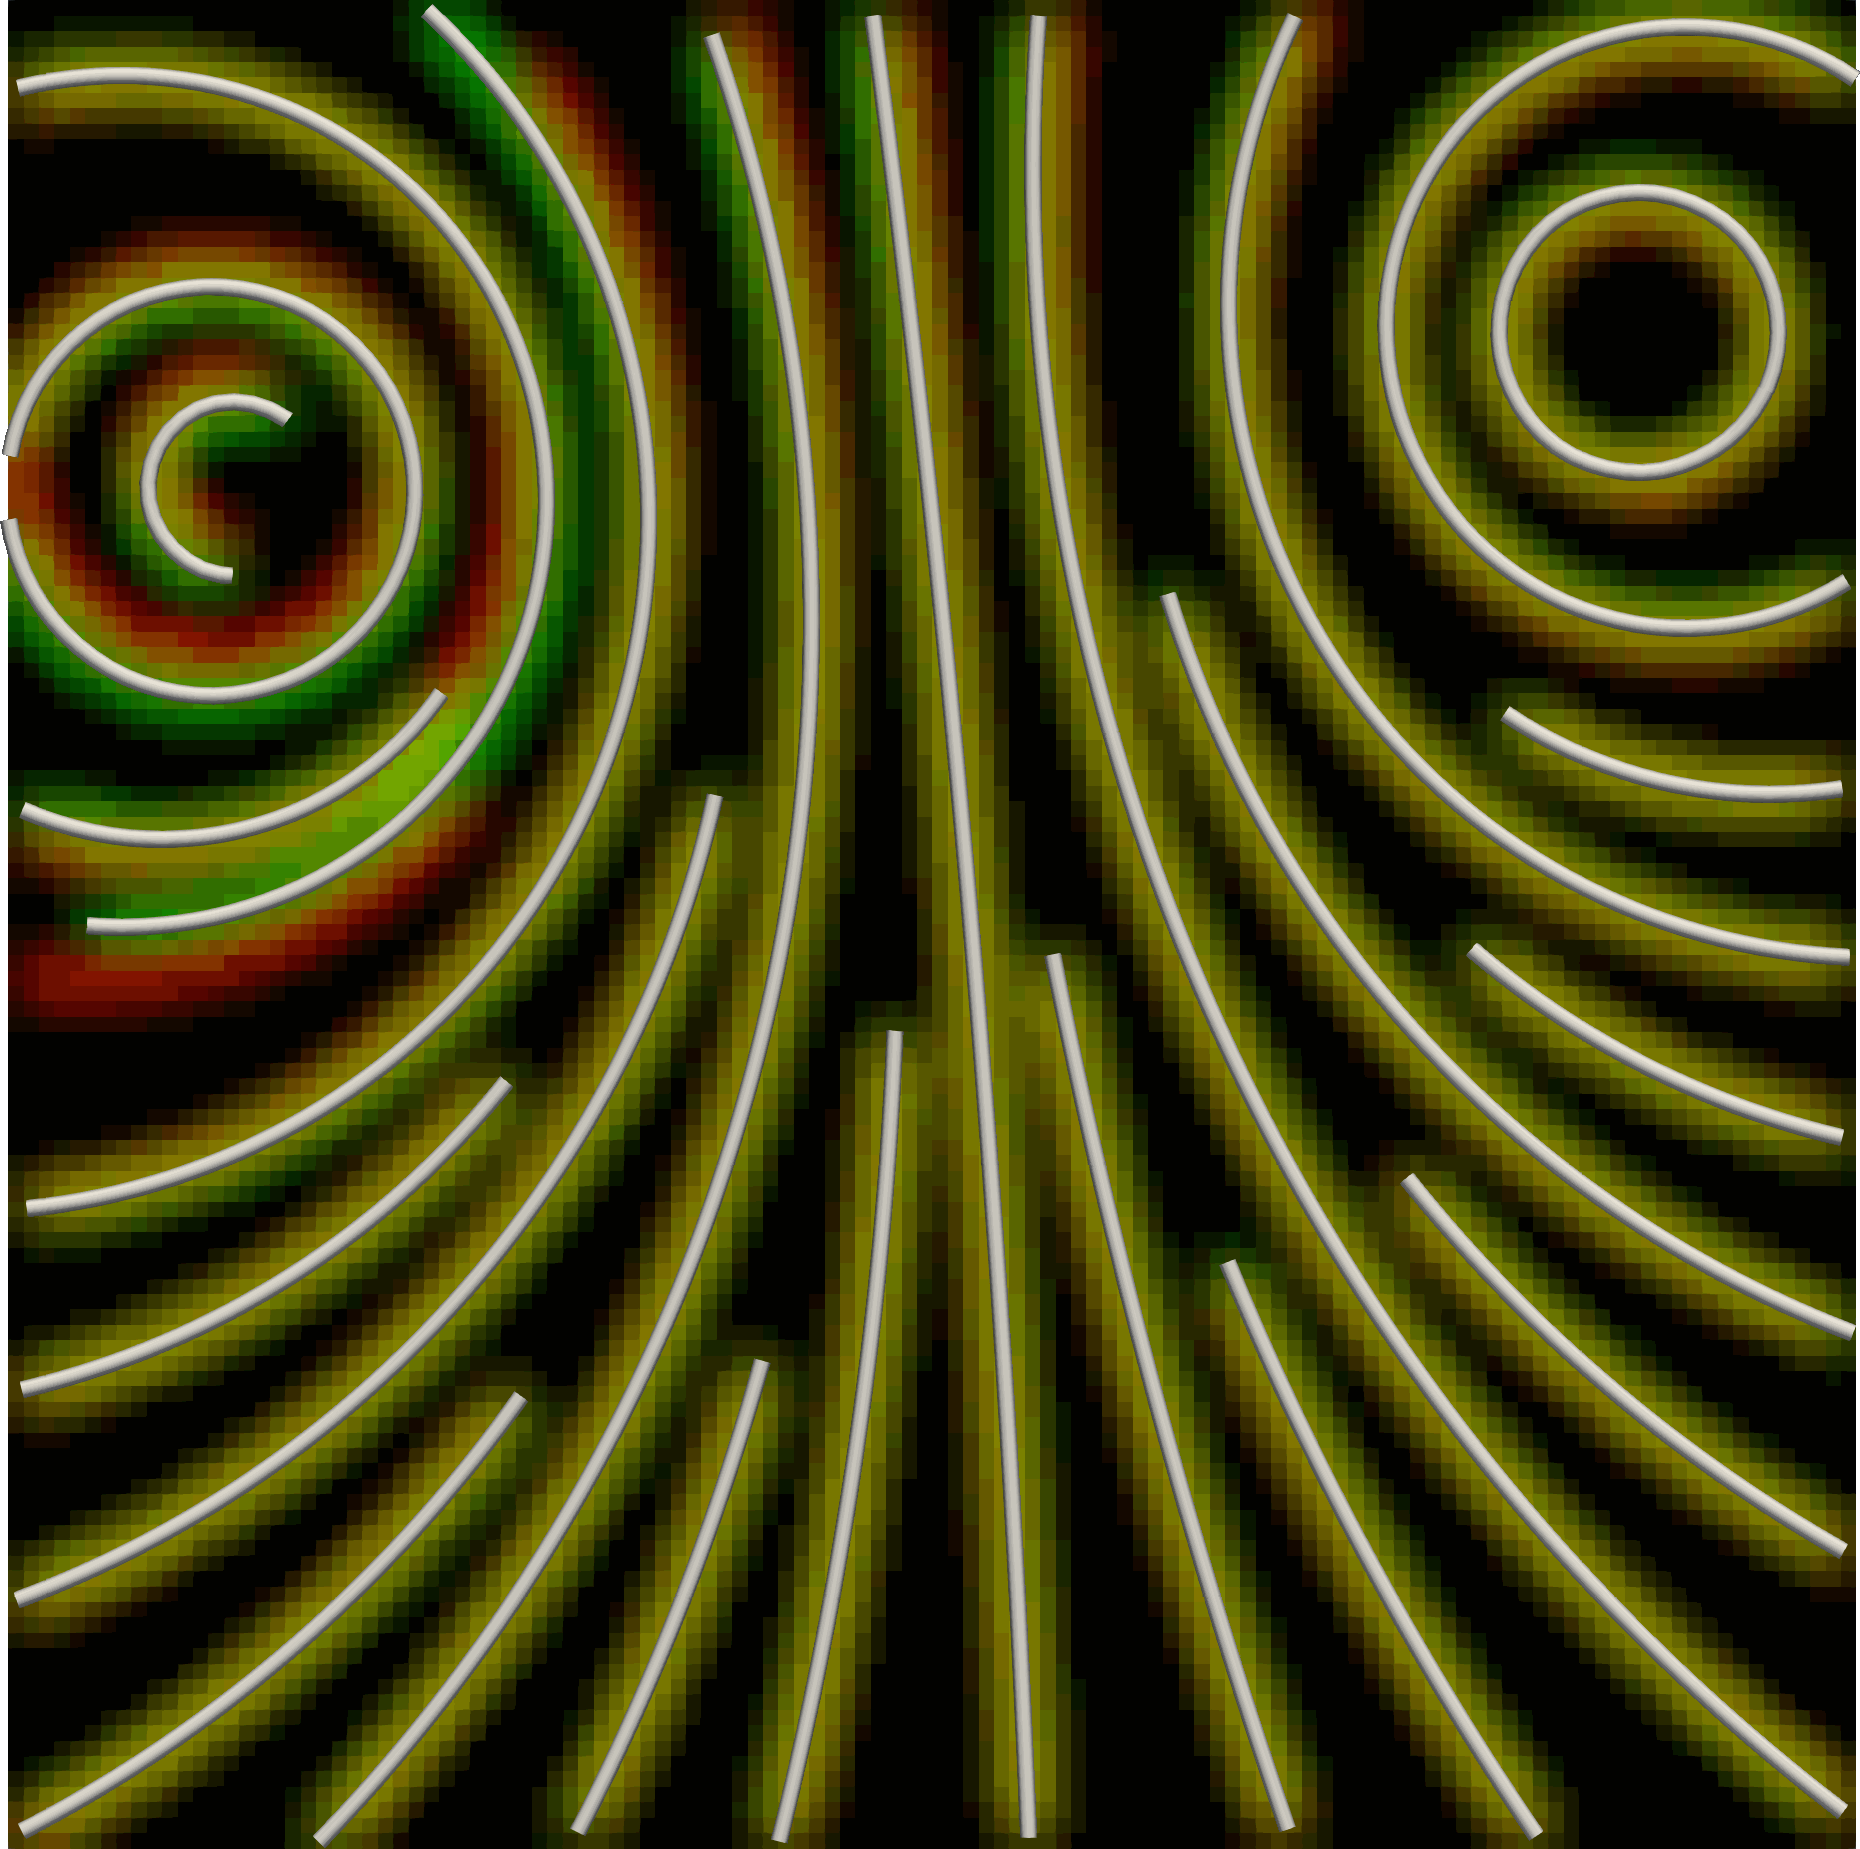
\includegraphics[scale=.055]{figures/AlphaStudy/Gyro33C.0004.png}
        \end{subfigure}
        \caption*{(d)}
    \end{subfigure}
    \caption{
        Comparison of different $\alpha$ values between the first five steps for an unsteady version of the double gyro field from \cref{fig:energydevelopment}.
        Each row represents five time steps and for each step, the left vortex moves down by $3\%$ of the image height.
        (a): With $\alpha=0$ most lines have low coherence and field movement is hard to notice between frames.
        (b): $\alpha=1/3$, TBD
        (c): $\alpha=2/3$, Good coherence in most regions, some strong changes remain
        (d): $\alpha=1$, Even better coherence with only slight changes, even in areas of field movement.
    }
\end{figure}

\subsection{Parameter Study for $\alpha$}
Since $\alpha$ drives how similar we want our images to be vs. how much we care about spatial placement and uniformity,
we briefly look at some examples for extreme cases and more moderate choices, examining some notable differences.
We start with a double vortex field, where the left vortex undergoes a downward motion. The distance travelled between each time step
is exactly 3\% of the image height.\\
In figures (a - d), we set $\alpha=0$, and the streamlines move sporadically with time coherence only being achieved by chance
and in areas almost completely unaffected by the change.
For (e - h), $\alpha=1/3$. We can immediately see some improvements, as the center is becoming more stationary.
The footprints overall gain a more compact appearance, as green and yellow parts aren't as far apart as they were previously.
The optimal range is reached somewhere around $\alpha=2/3$ (i - l), 
most of the footprints are now yellow with only slight divergence in areas not affected by the $y$-shift of the vortex.
At the same time, we preserve an even appearance of line spacing without particularly bunched or sparse areas.
For high values of $\alpha$ (m-p), we can tell that the image has become a lot worse compared to before.
We see large empty spaces, where lines cannot be drawn anymore due to the strong energy punishment inflicted by $E_t$ having such high weight.
These spaces can only increase in size as lines cannot grow past the previous footprint.
If the field changes further, the line length decreases in order to still fit the footprint left behind, causing less overall line presence every step.
We conclude that a good starting value for $\alpha$ would be in the $[0.5, 0.75]$ range.
This avoids the sharp decline in spatial quality, while still retaining good control over the placement to make the streamlines remain time coherent.

% An example for the coloring and $\alpha=0$ can be seen in \cref{fig:paramstudy1} (b-d).
% The divergence between the new and old streamline happens due to there not being any bias,
% therefore the slight changes made from random movement decide which side of the gyre it ends up on.
% In \cref{fig:paramstudy1} (e) we see the same line being generated for two successive frames.
% Because of the slight bias from the overlap of the initial seed (b) and the previous finished streamline's footprint,
% we have a gradient to move along toward better placement w.r.t time coherence.
% We have generated (e) 20 times, 18 of which ending up on the right.
% This small inaccuracy is a direct result from 


% Seeds resulting from shattering are shown in magenta, and are drawn after the footprints.


% \subsubsection*{Issues}
% Using only the brightness for coaxing is not ideal.
% This is mainly due to the fact that two neighboring parallel segments will not have the bright spots at their individual center,
% but rather at their combined center.
% Placing new lines there would cause one line to move right into the center of the previous lines,
% introducing a definite jump of both lines and impeding time coherence.
% This effect can be negated by changing the radius $R$ of our low-pass filter we use
% when comparing to the previous frame.
% This means that we cannot reuse $(L\ast I)$ for $E_0$ and $E_1$, and comes at a high cost:
% Since we use two different versions of $L$, and computing $L\ast I$ is by far the most expensive task in this algorithm,
% the runtime will increase by a factor of approximately two.
% We can reduce this cost by changing the computation of the low-pass filter:

\newpage

\begin{figure}[ht!]
    \centering
    \begin{subfigure}[b]{.3\textwidth}
        \centering
        
\includegraphics[scale=.08]{figures/Shatter/3Lines.png}
        \caption*{(a)}
    \end{subfigure}
    \begin{subfigure}[b]{.3\textwidth}
        \centering
        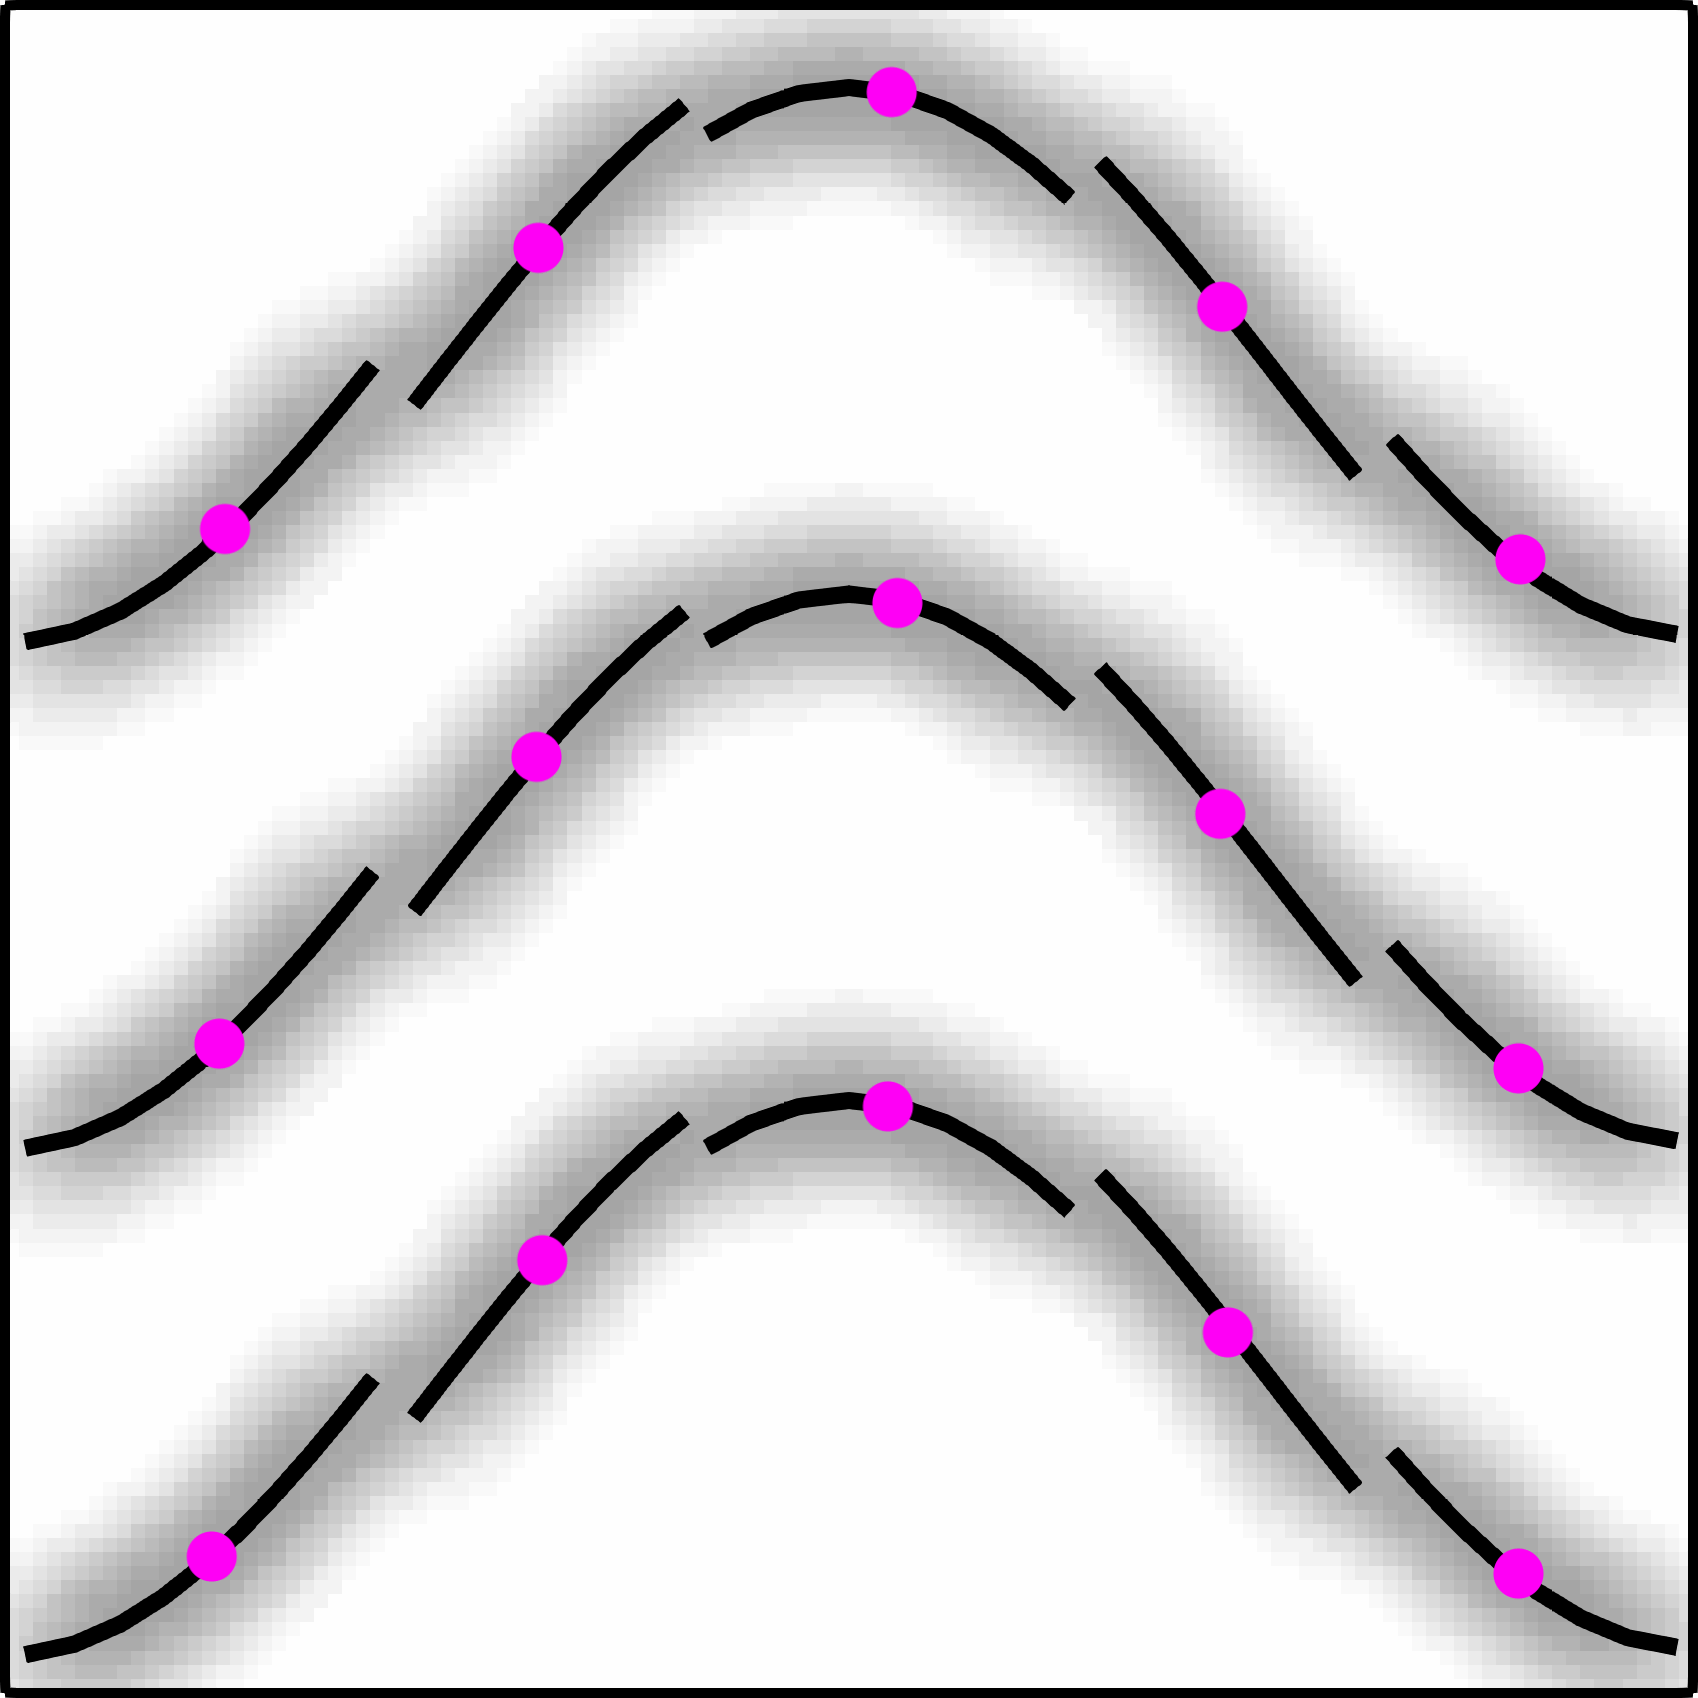
\includegraphics[scale=.08]{figures/Shatter/15Lines.png}
        \caption*{(b)}
    \end{subfigure}
    \begin{subfigure}[b]{.3\textwidth}
        \centering
        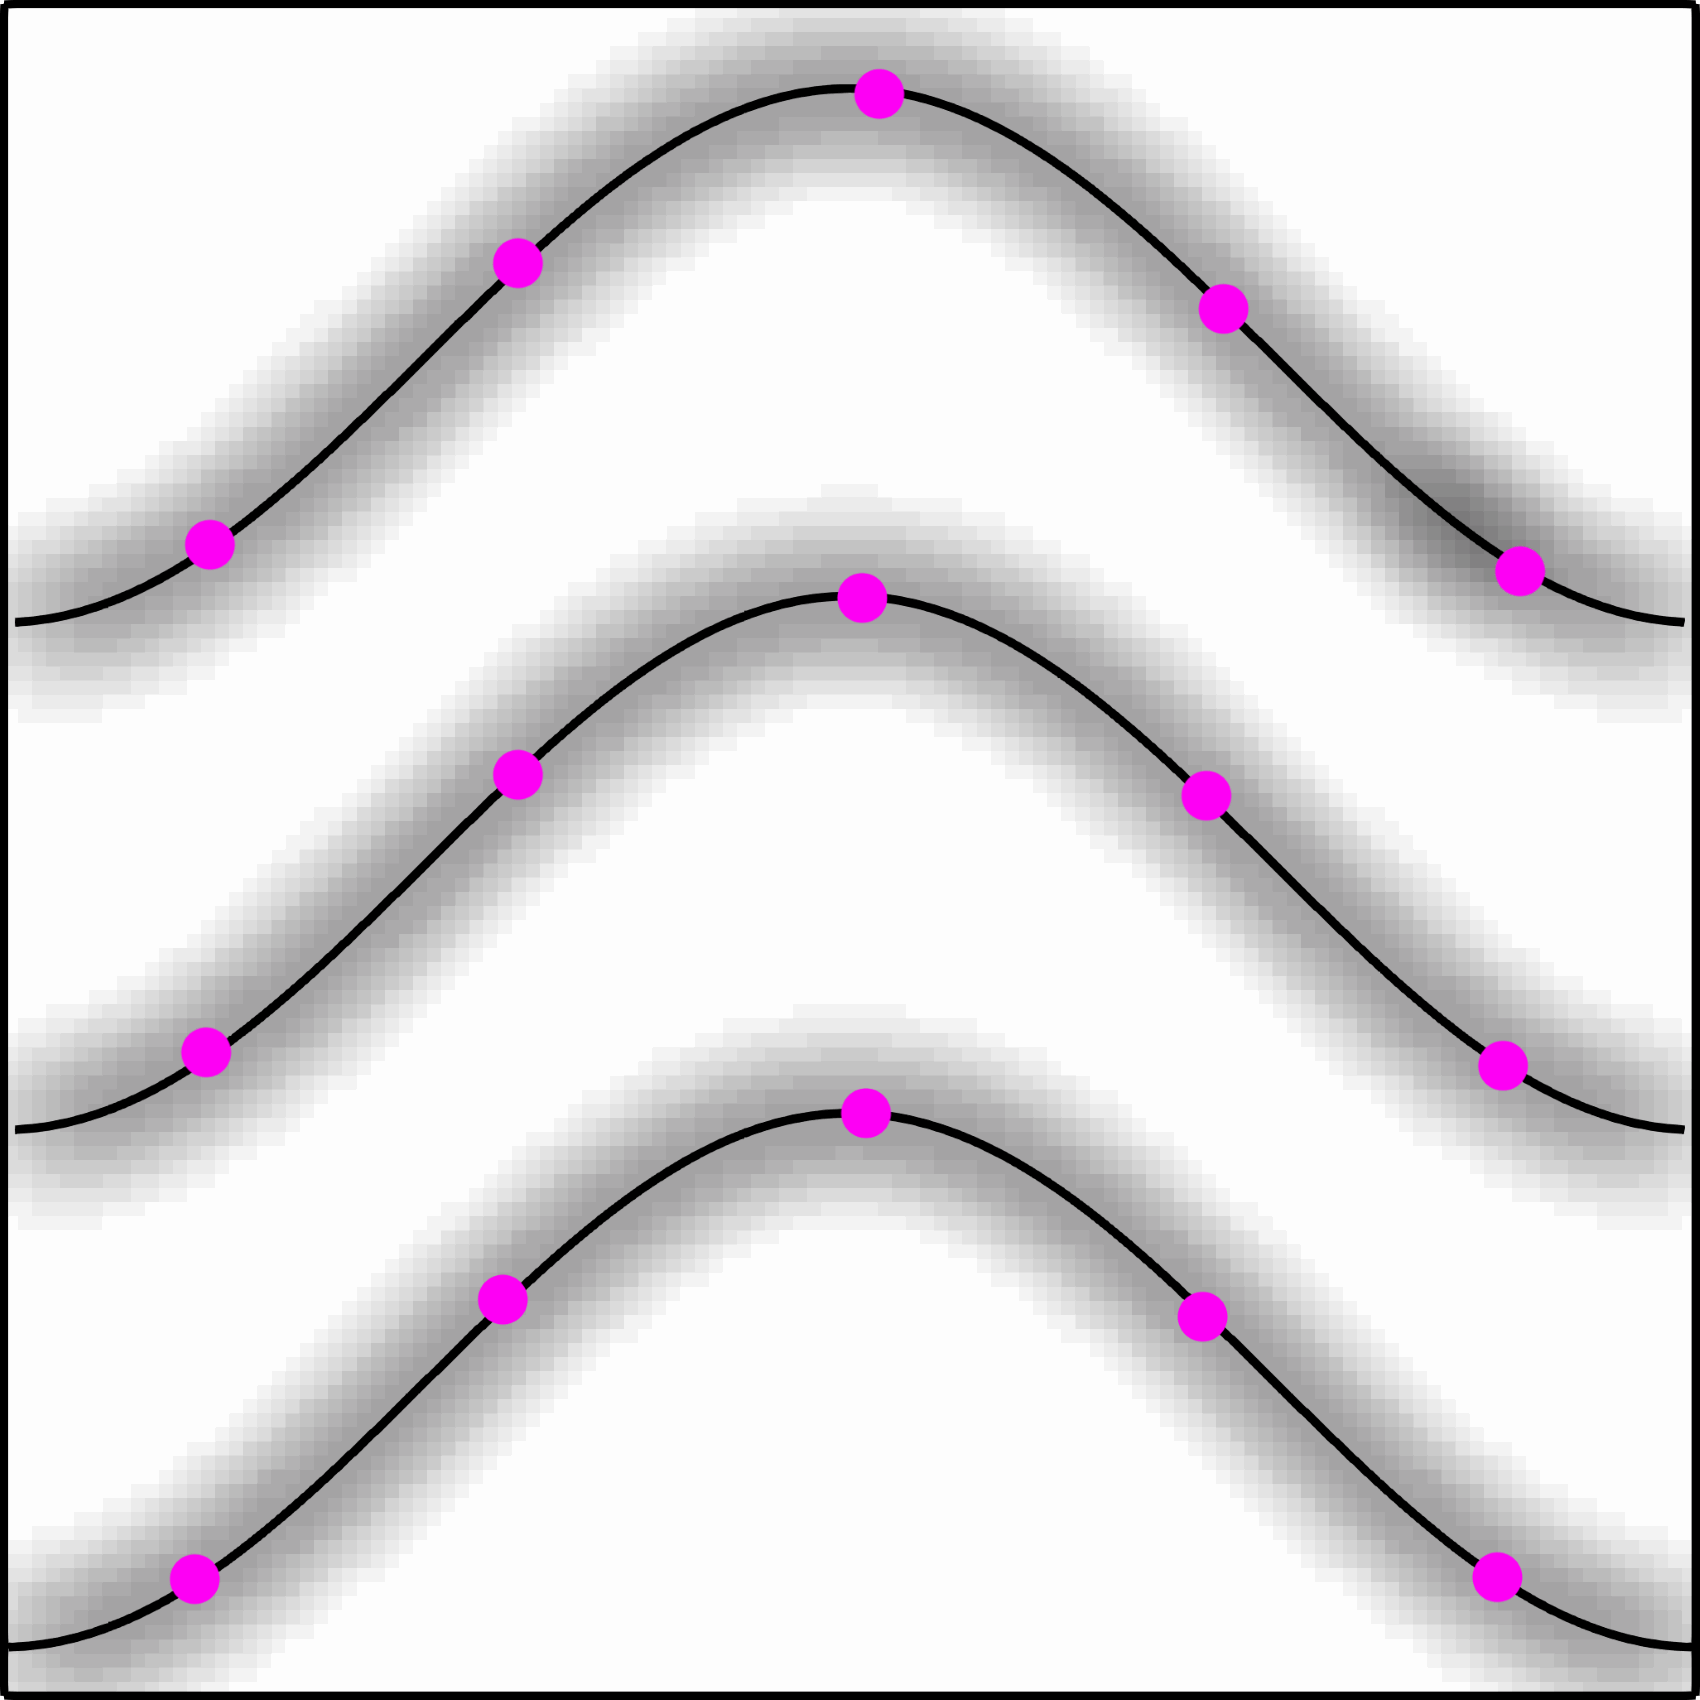
\includegraphics[scale=.07]{figures/Shatter/3LinesRejoin.png}
        \caption*{(c)}
    \end{subfigure}
    \caption{
        (a): Three streamlines after being optimized.
        (b): To make the individual shards visible, we change the field's amplitude slightly.
        The shards' seeds are the center of the streamlines in (b), and all lie on one of the streamlines in (a).
        (c): The lines quickly rejoin when re-drawn in the same field used in (a).
        We used slightly thinner lines to better show the seeds (thin black dots on the streamlines),
        and to make it more visible that the lines do not simply overlap but actually rejoin.
    }
    \label[figure]{fig:rejoin}
\end{figure}


\subsection{Shattering}
At the end of a time step's optimization phase, we break every streamline apart into smaller streamlets we refer to as \textit{shards}.
We start by dividing the parent line length-wise into sections which equal the length of the starting lines.
The shards are assigned a seed in the middle (lengthwise) of these intervals, and their length equals the line start length.
If the parent line has some length remaining because it was not perfectly divisible by the start length, the last shard's length will be shorter.
This leaves each former streamline with the appearance of being dashed with each fragment having its own seed, and can be seen in \cref{fig:rejoin} (b).
The shards then act as the initial seeding strategy for the subsequent timeframe; the regular grid is only used for the first frame.
This way, we obtain many seeds that, if the field does not change too much, will merge back into the line they came from, as can be seen in \cref{fig:rejoin} (a) and (c),
saving iterations that would be needed for new seeding and lengthening in these regions.
If the field \textit{does} change, some segments will still reconnect and therefore keep their temporal coherence,
whereas areas of strong fluctuation will connect to different seeds.
This results in changes being limited to parts where a streamline change is necessary,
providing extra lines in these areas while not affecting streamline trajectory too much on a global level.
\newpage

\begin{figure}[ht]
    \centering
    \begin{subfigure}[b]{.32\textwidth}
        \centering
        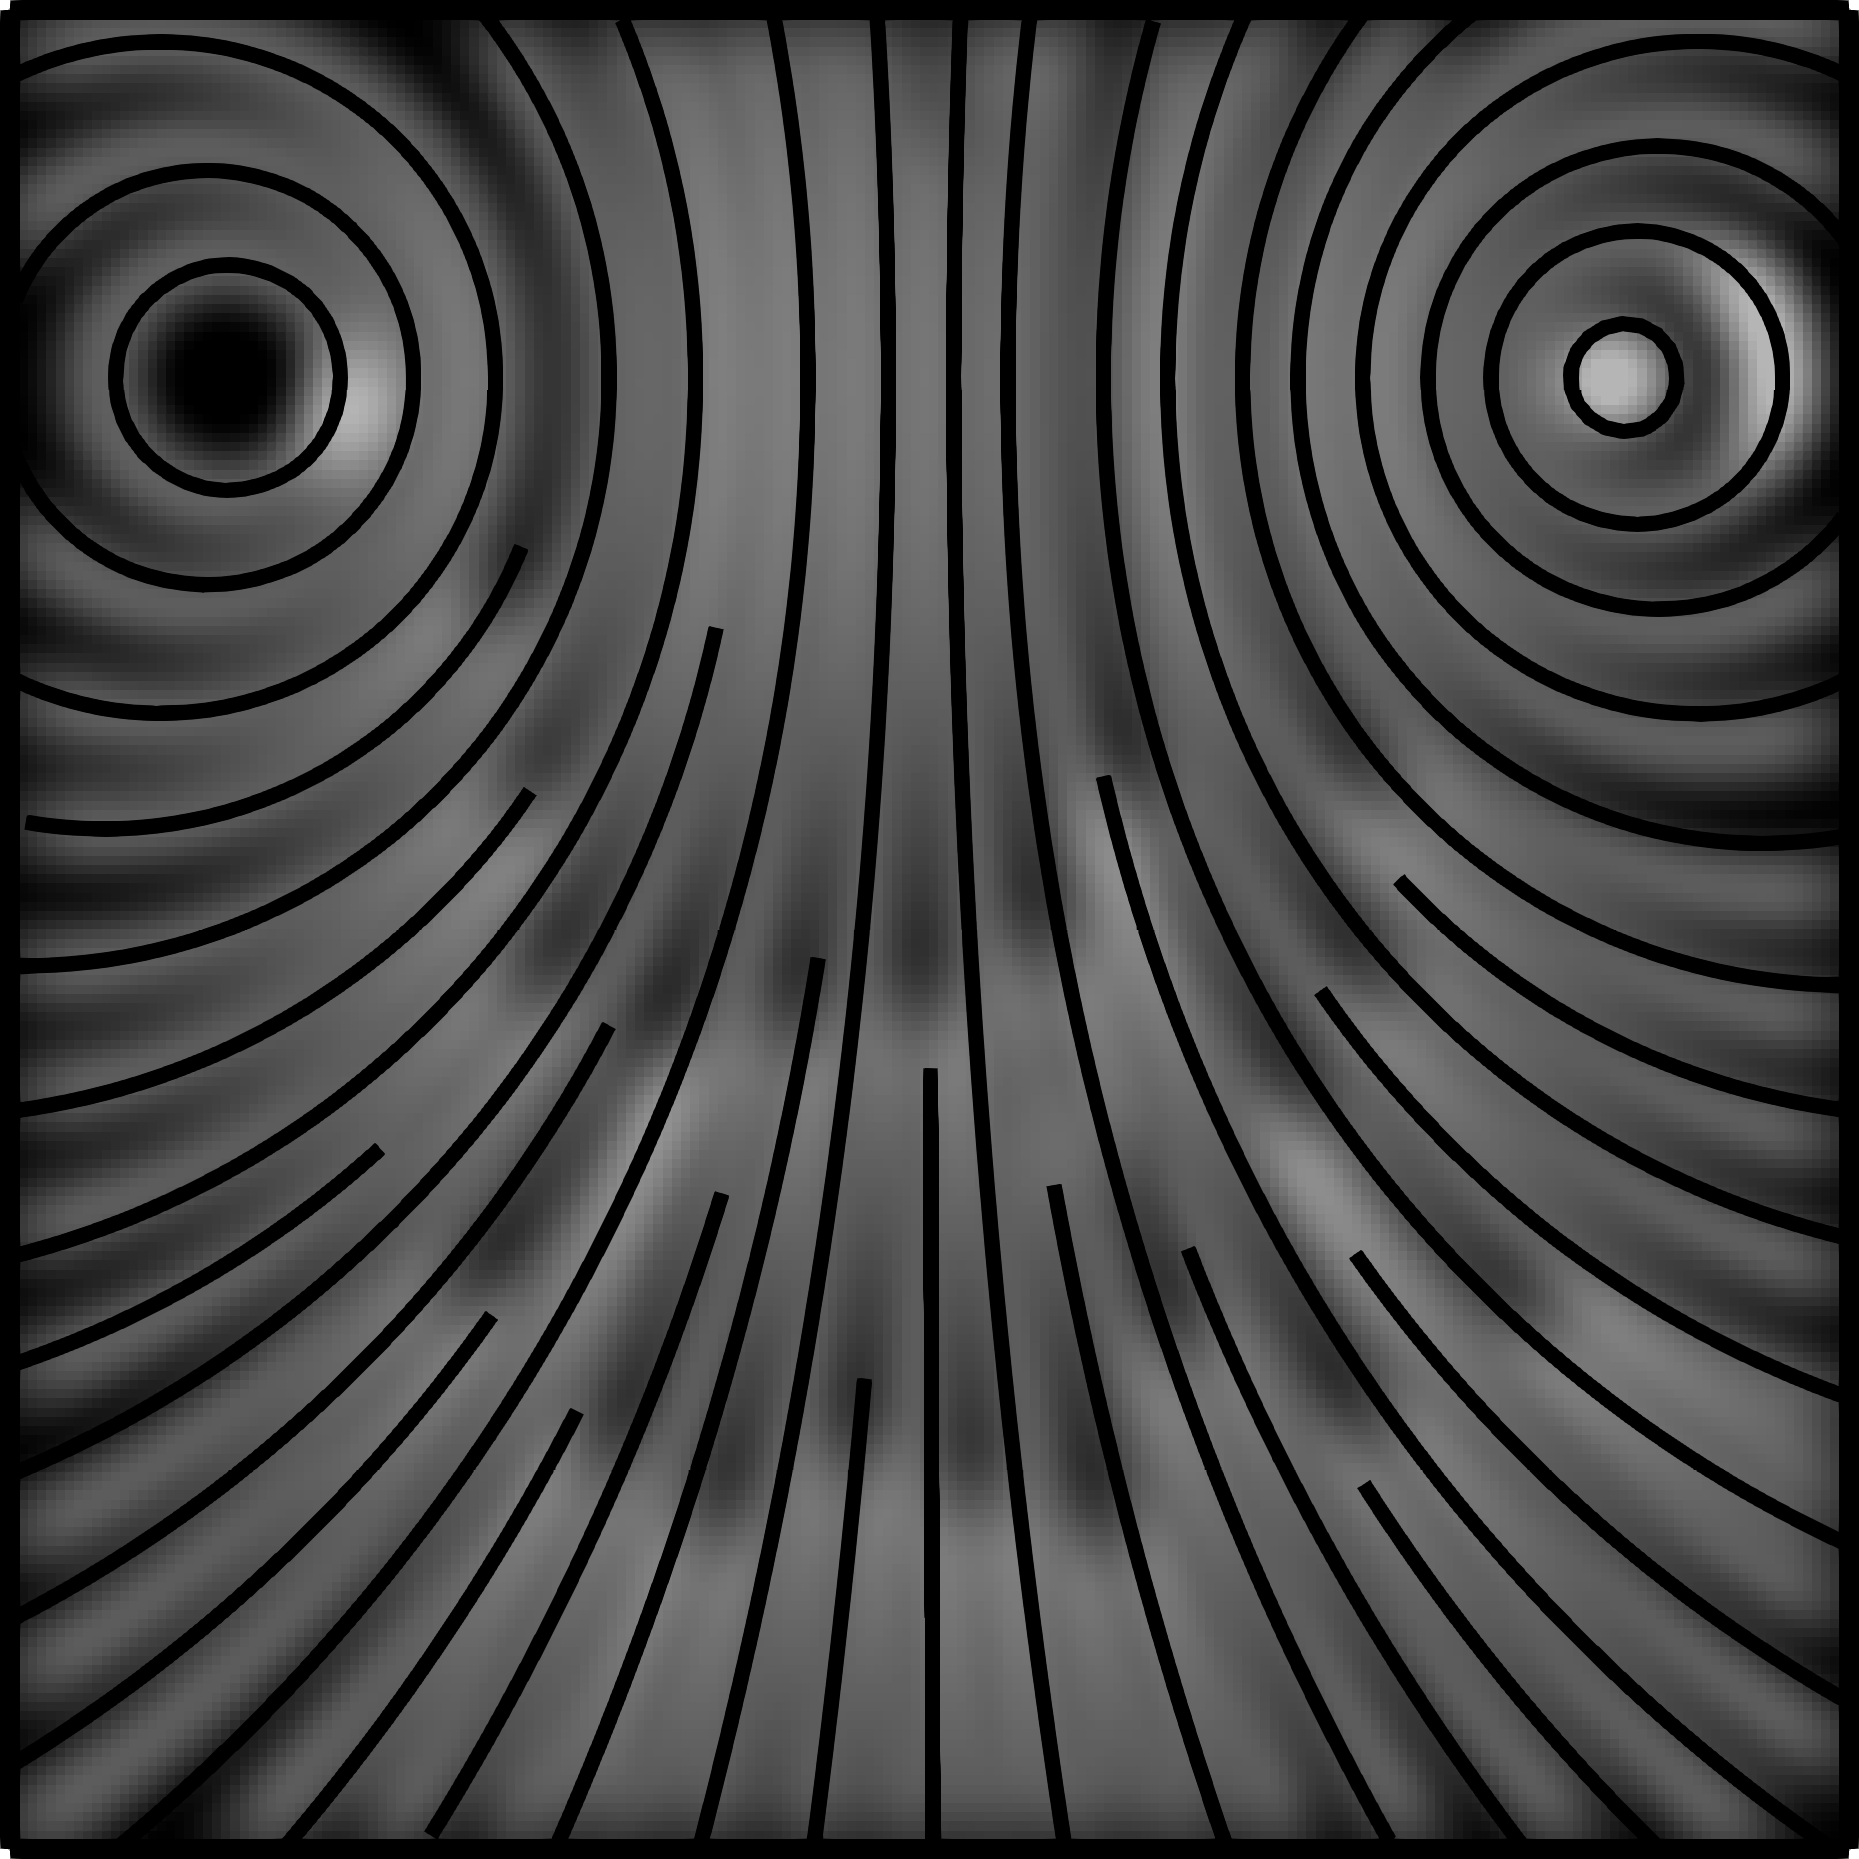
\includegraphics[scale=.08]{figures/TBGyro.png}
        \caption*{(a)}
    \end{subfigure}
    \begin{subfigure}[b]{.32\textwidth}
        \centering
        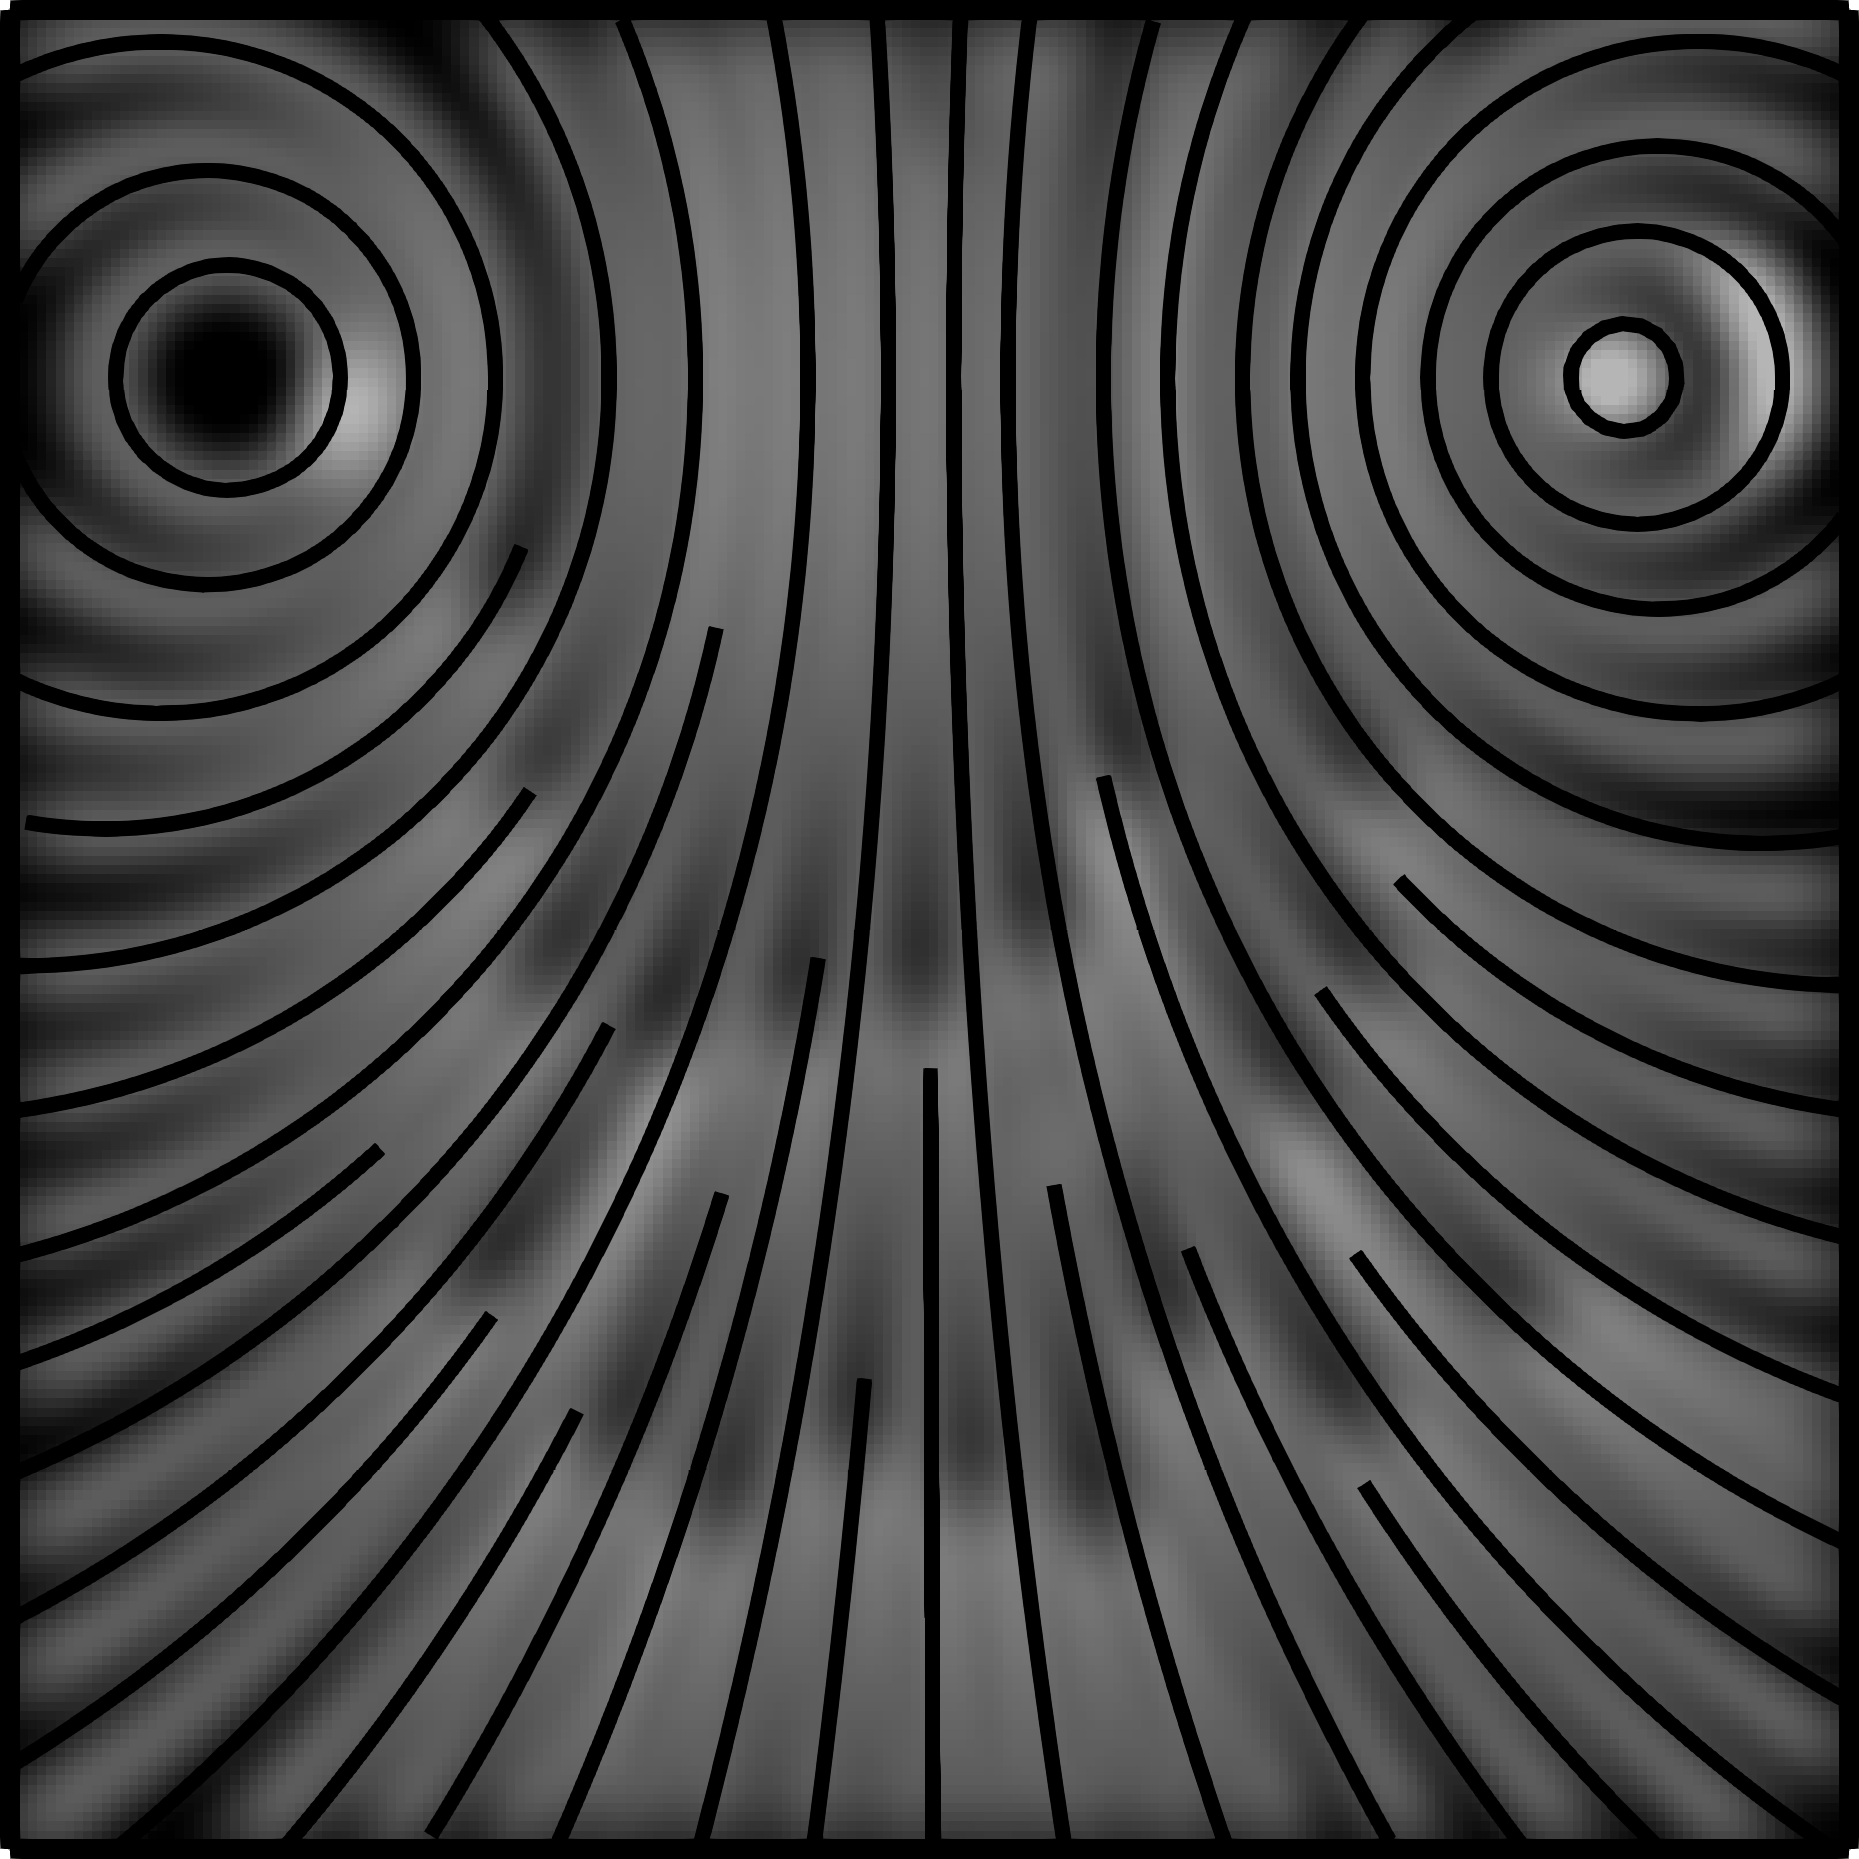
\includegraphics[scale=.08]{figures/TBGyro.png}
        \caption*{(b)}
    \end{subfigure}
    \begin{subfigure}[b]{.32\textwidth}
        \centering
        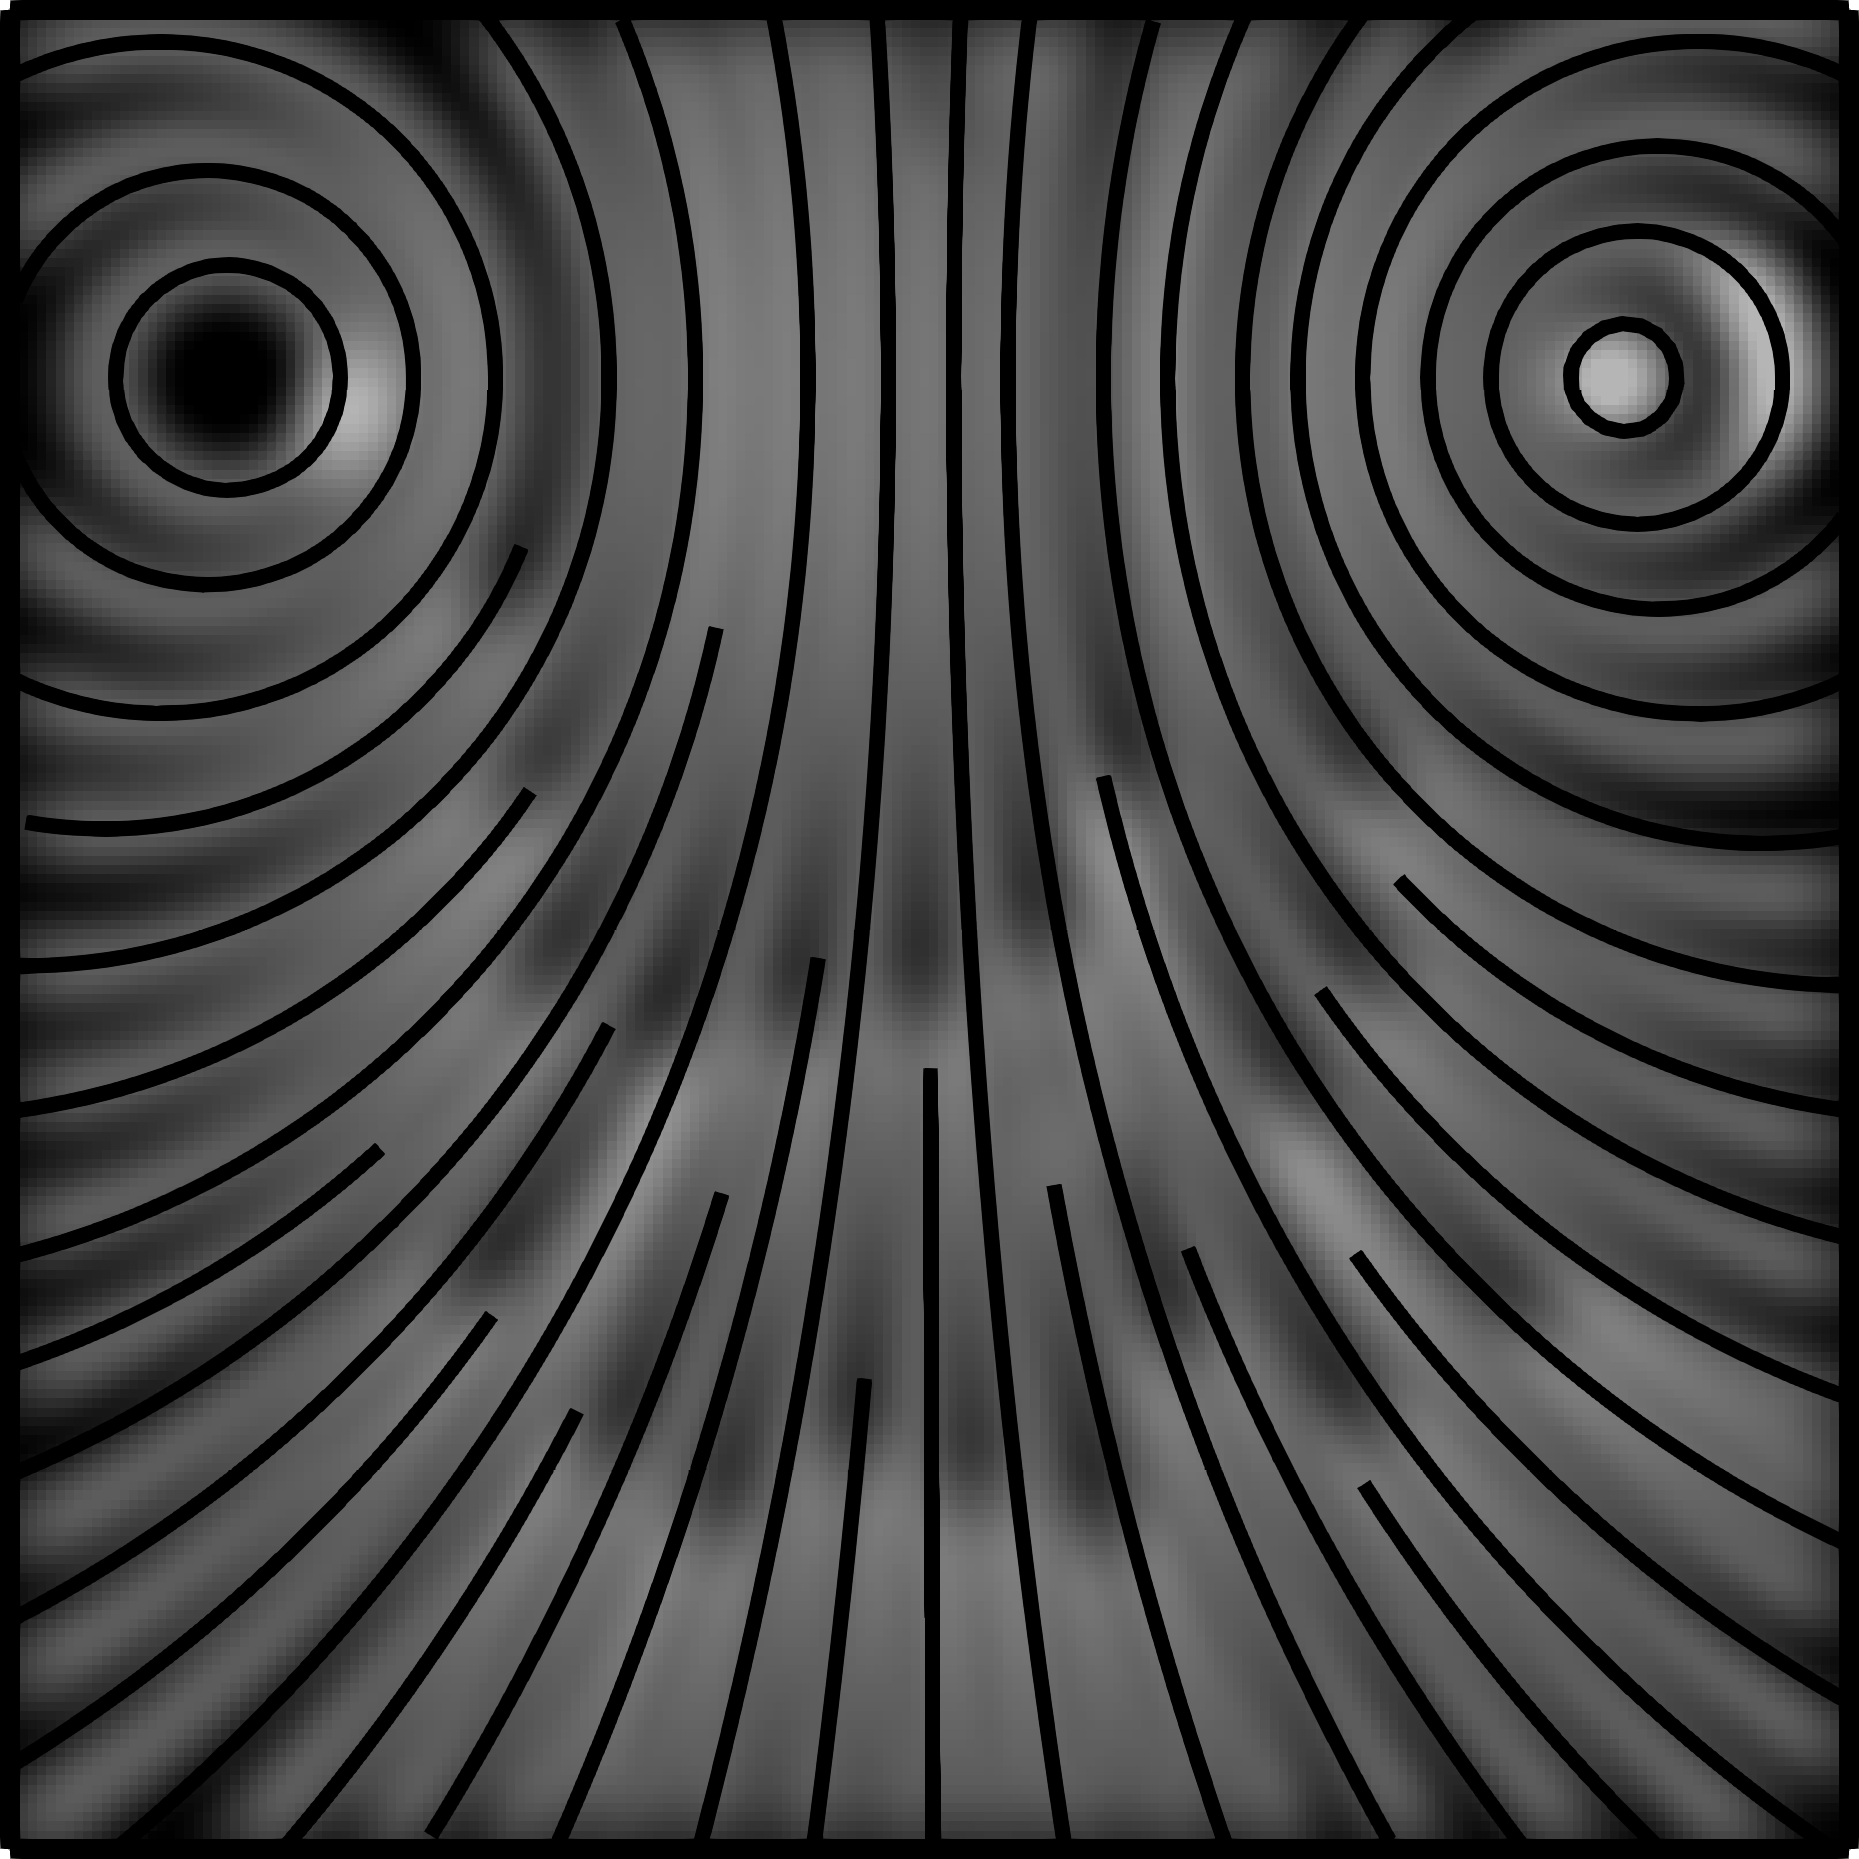
\includegraphics[scale=.08]{figures/TBGyro.png}
        \caption*{(c)}
    \end{subfigure}
    \caption{
        (a): Two time steps without shattering.
        (b): Two time steps with shattering.
        (c): Total energy vs iteration step for (a) and (b).
    }
    \label[figure]{fig:combined}
\end{figure}

\subsection{Combining Shattering and Coaxing}
Combining shattering and coaxing, we obtain a more reliable way of generating streamlines according to the footprint left behind by the last frame.
The seeds created during the shatter process all lie inside the footprint left behind by the previous streamline path.
Due to the coaxing function of the modified energy measure, it is unlikely that they will leave this valley solely due to the random movements of relaxation.
A change in the field is necessary in order to overcome the weight of the time coherence, making the line move or grow outside the previous footprint.
Due to the seeds being held in place in this way, it is very likely for them to re-join to form the same lane they originated from.
If the field changes drastically in this region, the seeds can not fully connect to each other anymore, and will instead gravitate to a different footprint,
forming long patches of coherent lines whenever possible while still allowing relaxation to ensure good spatial distribution.\\
In \cref{fig:combined} (c),
we see that joining shards to form the streamlines is significantly faster than generating them anew.






At first, a heuristic criterion for temporal coherence between stream lines is defined.
Then ...


\begin{itemize}
    \item old implementation
    \item issues, why sth else was used
    \item turk and banks
    \item why turk and banks? (spacial coherence?)
    \item time coherence definition
\end{itemize}

We have chosen to keep most of these actions as-is, the only difference introduced is
a change to how the lengthening and shortening is done. 
Instead of the two binary choices of lengthen/shorten and front/back, which only add/subtract a tiny bit at a time,
we decided to choose a segment count at random between -5 and 5 for each end.
This allows faster growth/shrinking (and hence faster convergence) while still preventing overlaps.

\subsection{Initial Seeding}
We prepare the image for the optimization routine by adding many streamlets with seeds on a regular grid to the image.
This can also be done randomly yielding similar image quality,
however strided access is more efficient with little to no benefit for the latter.

\subsection{Oracle}
The oracle from Turk and Bank's algorithm is used to suggest shorten/lengthen and move operations.
Our oracle focuses on shorten/lengthen suggestions only.

\subsection{Adding time coherence}
We added two important modifications to the aforementioned algorithm to make it partially time-coherent.
The first modification affects how seeds are chosen in the beginning of an optimization pass; the second affects
how the energy measure is computed and lines are guided toward their final positions.

  %%%%%%%%%%%%%%%%%%%%%%%%%%%%%%%%%%%%%%%%%%%%%%%%%%%%%%%%%%%%%%%%%%%%%%%%
\chapter{Implementation}
\label[section]{sec:implementation}
%%%%%%%%%%%%%%%%%%%%%%%%%%%%%%%%%%%%%%%%%%%%%%%%%%%%%%%%%%%%%%%%%%%%%%%%
This chapter briefly mentions the used libraries, and focuses on the initial implementation of - and iterative additions to - the proposed algorithm.
\section{Libraries}
The algorithm is implemented in Python3.10, and heavily relies on three libraries which are not part of the Python3.10 standard library:
\begin{itemize}
    \item ParaView v.5.12.0: A Scientific visualization software, combining data science and interactive visualization while providing custom algorithm support via the VtkPythonAlgorithm base class.
    \item VTK v.9.3.20231030 : The library used to manage anything related with the data to be visualized in ParaView.
    \item NumPy v.1.23.4: Widespread data manipulation/scientific computing library, which is used to edit the data encapsulated by VTK's objects.
\end{itemize}

\section{Time Coherent Algorithm Implementation}
Using the ``Visualization Tool Kit (VTK)'' and the ``Parallel Viewer (ParaView)'' provides a broad spectrum of available algorithms.
The most important components used are briefly listed in the following section,
the final algorithm design is delivered afterwards in \Cref{sec:impdesign},
and we conclude this chapter with a complexity analysis in \Cref{sec:impcomplexity}.

\subsection{Vital External Software Components}
\label[section]{sec:impvital}
\paragraph*{VTK Pipeline} While an extremely involved topic with dozens of hours to be spent on reading,
we try to summarize it as follows:
The VTK pipeline consists of three types of objects: Sources, filters, and sinks. Sources create data, filters modify it, and sinks display it.
Each object has input and output ports, how many of which it has decides its membership of one of the above groups.
A simple workflow to visualize a vector field would be: Vector Field Source $\rightarrow$ Line Geometry Generation $\rightarrow$ Screen Rendering.
\paragraph*{vtkPythonAlgorithm} This class is intended as a base class for writing custom algorithms in either of the three categories.
We use this twice: Once for a group of vector field sources to test our implementation with, and for the algorithm itself.
In the former case, we use it as a source, in the latter as a filter. The relevant method in this class is called "RequestData", which is passed an information object.
We can modify this object in order to pass data forward (and backward, though we do not need this) through the pipeline.
\paragraph*{vtkImageData} Objects of type vtkImageData hold a grid defined by 2 3-vectors: The extents (number of points in each direction), and the spacing (how far points are apart in X/Y/Z direction).
Every point on this rectilinear grid can have scalars or other objects assigned, like a velocity as a 3D vector.
In our case, we use it exactly in this way:
Points are assigned velocities, which are then interpolated as needed.
\paragraph*{vtkStreamTracer} The vtkStreamTracer class is a filter with two inputs: We provide it with a vector field (vtkImageData) object and a point, which it then integrates through the field.
The relevant output for us is the list of points making up the streamline that it returns.
\newpage
\subsection{Algorithm Design}
\label[section]{sec:impdesign}
Since we need two filters ($L_s, L_t$), and want them to act on different time steps, we have decided to implement the filtering and drawing subsystem as follows:
\paragraph*{FilterTarget} Effectively a wrapper for an image, allowing easier access to some properties.
It contains the brightness information of the image that guides our algorithm.
\paragraph*{Painter} This is the modifying actor for FilterTargets.
Painters use a configuration (line brightness, blur size, etc.)
and draw poly lines to the FilterTargets accordingly. This is how we distinguish between $L_t$'s and $L_s$'s radii.
\paragraph*{Filter} These objects contain a list of lines that make up the vector field image,
and orchestrate the assigned Painters and their respective configuration objects.
They also provide methods for adding/removing/modifying lines,
using a given energy function to determine their success.
They act as the binding agent for the logic modifying line placement and actually performing the change.
\paragraph*{FilterStack} This class is best used (though not enforced) as a singleton;
it manages two filter objects, one for the current,  and one for the last time step.
It also provides the energy methods as lambdas to the new filter added every time step.

This change compared to the original was necessary,
because we now want to manage multiple filters from different time frames at the same time.
It is even possible to make the filter change depending on how long ago it was created,
e.g. to not only use time coherence w.r.t the last frame,
or to allow effects like onion skinning of older frames' low pass images.

The entry point for this algorithm is, as with any vtkPythonAlgorithm,
the ``RequestData'' method (we leave out the other Request() methods for brevity).
We are provided the vector field via the vtkImageData object as input,
and start to set up our low-pass filter stack.

By setting up a filter with a config
(the standard config uses similar values as Turk and Banks' implementation), we create the $E_s$ part.
If we are not interested in time coherence,
this is all that is necessary for a line to be drawn filter-wise.
Otherwise, we simply add another config specialized to work well with $E_t$,
so our filter now has two configs, painters, and targets: One for $E_s$, one for $E_t$.

Drawing the lines themselves is done using NumPy's vectorization,
since we can use the NumPy-compatible vtkDataSetAdapter (DSA).
We use this to quickly obtain and transform the coordinates returned from the vktStreamTracer.
The drawing process is handled entirely by the Painter objects:
For a line $L$ containing $n$ seeds, we calculate the bounding boxes of $n-1$ segments,
padded by the filter radius.
Each pixel inside this rectangle has a number of vectorized calculations
performed in order to determine its brightness.
The brightness is evaluated using a precomputed grayscale table which we
interpolate via SciPy's RegularGridInterpolator, as this also supports vectorized access.
Once each segment's pixels are computed, we simply add them to the global line image.

Having finished the drawing process, we now look at the energy measure.
The filter stack hands over a lambda to the respective filter, with some arguments bound to their respective FilterTarget.
This way, we can dynamically change how the filter calculates values based on the gray scale values form the bound targets.
If, e.g., we do not have an old filter yet, we cannot use the \textit{coaxing} strategy.
Therefore, we simply leave the argument bound to "None" when passing it to the first filter.


\subsection{Complexity Analysis}
\label[section]{sec:impcomplexity}
\paragraph*{Line Integration}
We heavily rely on the vtkStreamTracer (see \Cref{sec:impvital}),
which we configured to use the Runge-Kutta-4 solver.
RK4 uses a complexity of $O(n)$, with $n$ being the number of integration steps taken.
Hence, obtaining the sample points of a single streamline of length $n$ is of complexity $O(n)$.

\paragraph*{Drawing a Line Segment}
When computing the footprint of a streamline, we do so segment by segment.
A segment footprint's pixel count $f$ is defined by two values:
The filter radius $r$ and the maximum step length $l$.
The maximum cost of drawing a segment is therefore a constant, and we write this cost as $c$.

\paragraph*{Drawing a Line}
If the line consists of $n$ segments each costing a maximum of $c$, the cost is simply $O(n)$.
This remains unchanged when including the cost of integration, as we still get $O(2n) = O(n)$.

\paragraph*{Generating a Streamline}
Lines start at very low length, and need to grow and shift, causing them to be redrawn over and over.
Generating a single line by letting it grow means we re-evaluate it as often as necessary.
We need to draw $O(0.5\cdot n^2)=O(n^2)$ segments to reach a length of $n$,
combining this with the cost of drawing a length-$n$ line, we arrive at $O(cn^2)=O(n^2)$.
\\\\
The randomized operations all cause a line to be re-generated, but since its length remains, this is done
with $O(n)$. However, we do this fairly often, making the complexity w.r.t. segment size and iteration count
behave as if it were quadratic.

  %!TEX root = ../Thesis.tex

%%%%%%%%%%%%%%%%%%%%%%%%%%%%%%%%%%%%%%%%%%%%%%%%%%%%%%%%%%%%%%%%%%%%%%%%
\chapter{Results}
\label{chap:Results}


\begin{figure}[t]
  \subfloat[\label{fig:one}]{%
    \exampleDuck[width=0.45\linewidth]%
  }%
  \hfill%
  \subfloat[\label{fig:two}]{%
    \exampleDuck[width=0.45\linewidth]%
  }%
  \caption{Example for two~\protect\subref{fig:one} sub-figures~\protect\subref{fig:two}.}
\end{figure}

In \autoref{chap:Results}, \autoref{sec:section}, we will see bla, specifically in \autoref{sec:subsection} this will be emphasized. \Blindtext[2]
%%%%%%%%%%%%%%%%%%%%%%%%%%%%%%%%%%%%%%%%%%%%%%%%%%%%%%%%%%%%%%%%%%%%%%%%
\section{Section}
\label{sec:section}

\Blindtext[6]
%%%%%%%%%%%%%%%%%%%%%%%%%%%%%%%%%%%%%%%%%%%%%%%%%%%%%%%%%%%%%%%%%%%%%%%%
\subsection{Subsection}
\label{sec:subsection}

\Blindtext[3]
%%%%%%%%%%%%%%%%%%%%%%%%%%%%%%%%%%%%%%%%%%%%%%%%%%%%%%%%%%%%%%%%%%%%%%%%
  %!TEX root = ../Thesis.tex

%%%%%%%%%%%%%%%%%%%%%%%%%%%%%%%%%%%%%%%%%%%%%%%%%%%%%%%%%%%%%%%%%%%%%%%%
\chapter{Conclusion}

\Blindtext[16]
%%%%%%%%%%%%%%%%%%%%%%%%%%%%%%%%%%%%%%%%%%%%%%%%%%%%%%%%%%%%%%%%%%%%%%%%  

% This ensures that the subsequent sections are being included as root
% items in the bookmark structure of your PDF reader.
\bookmarksetup{startatroot} 
\backmatter
  
  \printbibliography
  
\end{document}